\chapter{Pruebas y resultados}
\label{cap:pruebas}

Este capítulo documenta una selección de pruebas automáticas del \textit{backend} del
sistema y una prueba de carga con cuatro sesiones. Se organiza así: el alcance de la
selección y los requerimientos que verifica, las restricciones de la base de datos que
comprueba, la prueba de carga, la verificación del sistema completo con un video real, las
pantallas de otras funciones, los límites de lo que no cubre y, al final, la validación del
clasificador.

% ============================================================
\section{Alcance y estrategia}
\label{sec:pruebas_estrategia}

Una prueba automática es un programa corto que ejecuta una parte del sistema y comprueba
que el resultado sea el esperado; se puede repetir en cualquier momento y avisa cuándo un
cambio rompe algo que antes funcionaba. El \textit{backend} usa JUnit~5, el marco de pruebas
estándar de Java. Las pruebas de este capítulo corren contra PostgreSQL, el gestor de bases
de datos relacionales del sistema, y no contra una base simulada.

Se documentan \textbf{77 pruebas seleccionadas del trabajo terminal}. Esas pruebas
levantan la aplicación completa contra una base PostgreSQL de pruebas, vacía y creada con
el mismo script de esquema que usa el sistema, y preparan y comprueban sus datos con
consultas directas. La excepción son 2 pruebas de la regla del último Administrador, que no
usan base de datos. Cada arranque verifica además que las entidades de la aplicación
coincidan con las tablas; si no coinciden, la aplicación no arranca.

Con la base de pruebas, las 77 pasan, sin fallos ni errores. Sin base de datos, 75 se
omiten y 2 corren. Las Figuras~\ref{fig:pruebas_corrida_con_base} y
\ref{fig:pruebas_corrida_sin_base} muestran la salida de ambas corridas.

\begin{sidewaysfigure}[p]
\centering
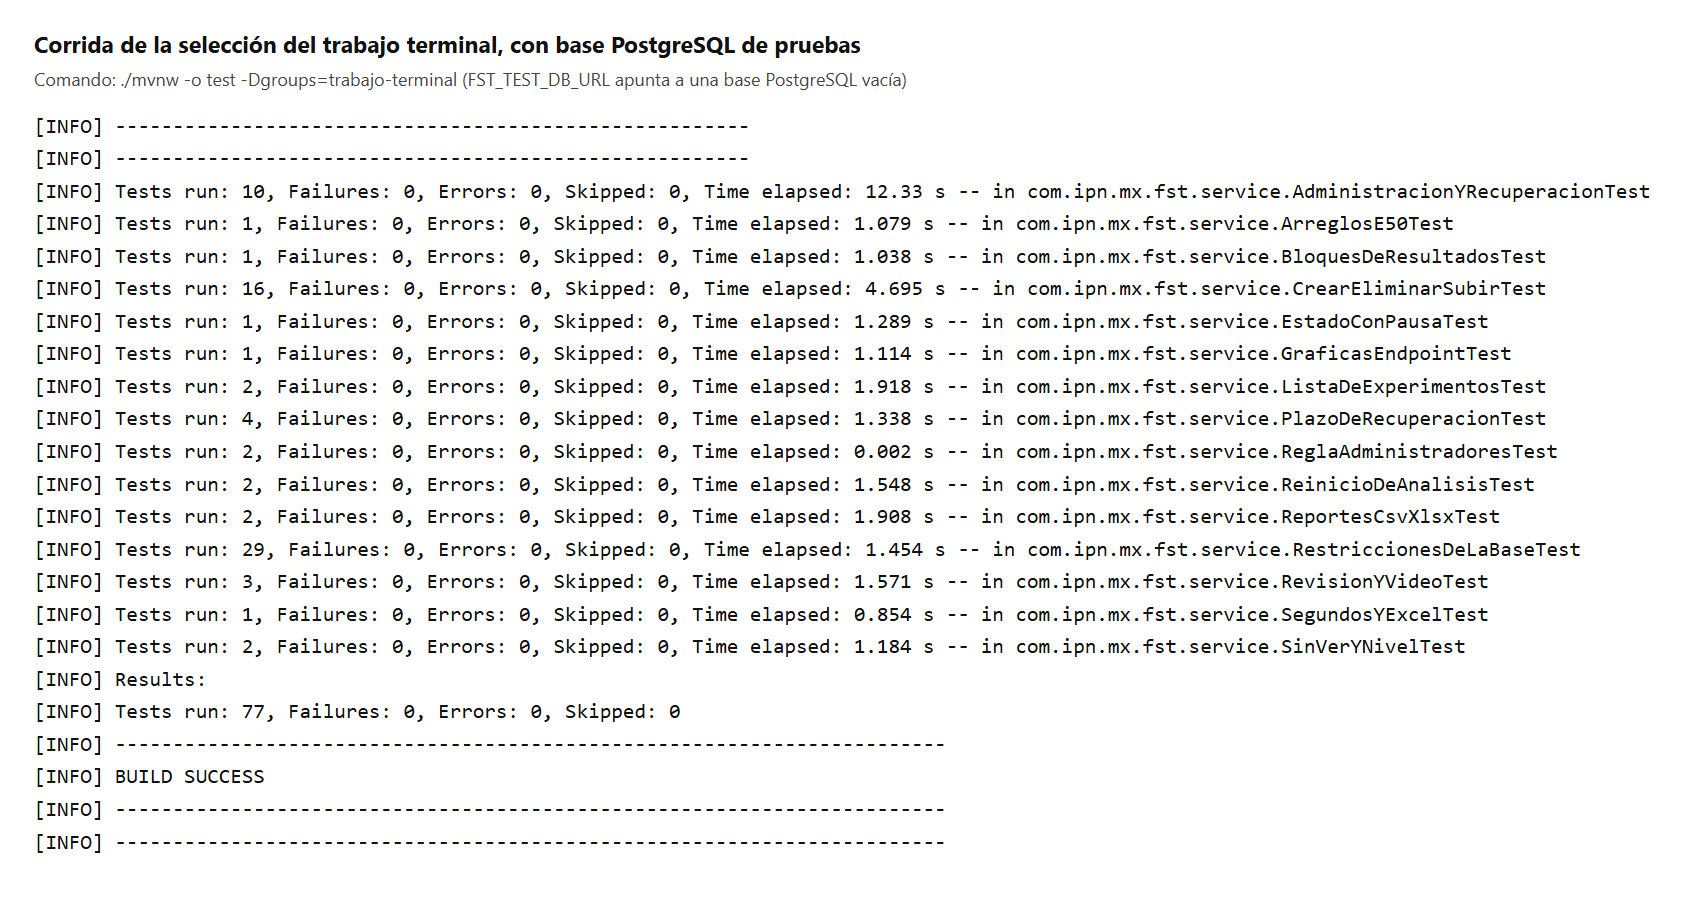
\includegraphics[width=\textheight, height=0.9\textwidth, keepaspectratio]{figures/pruebas/01_corrida_77_con_base}
\caption{Salida de la corrida de la selección con base PostgreSQL de pruebas, reproducida como texto a partir del registro de Maven y de los reportes de las pruebas.}
\label{fig:pruebas_corrida_con_base}
\end{sidewaysfigure}

\begin{sidewaysfigure}[p]
\centering
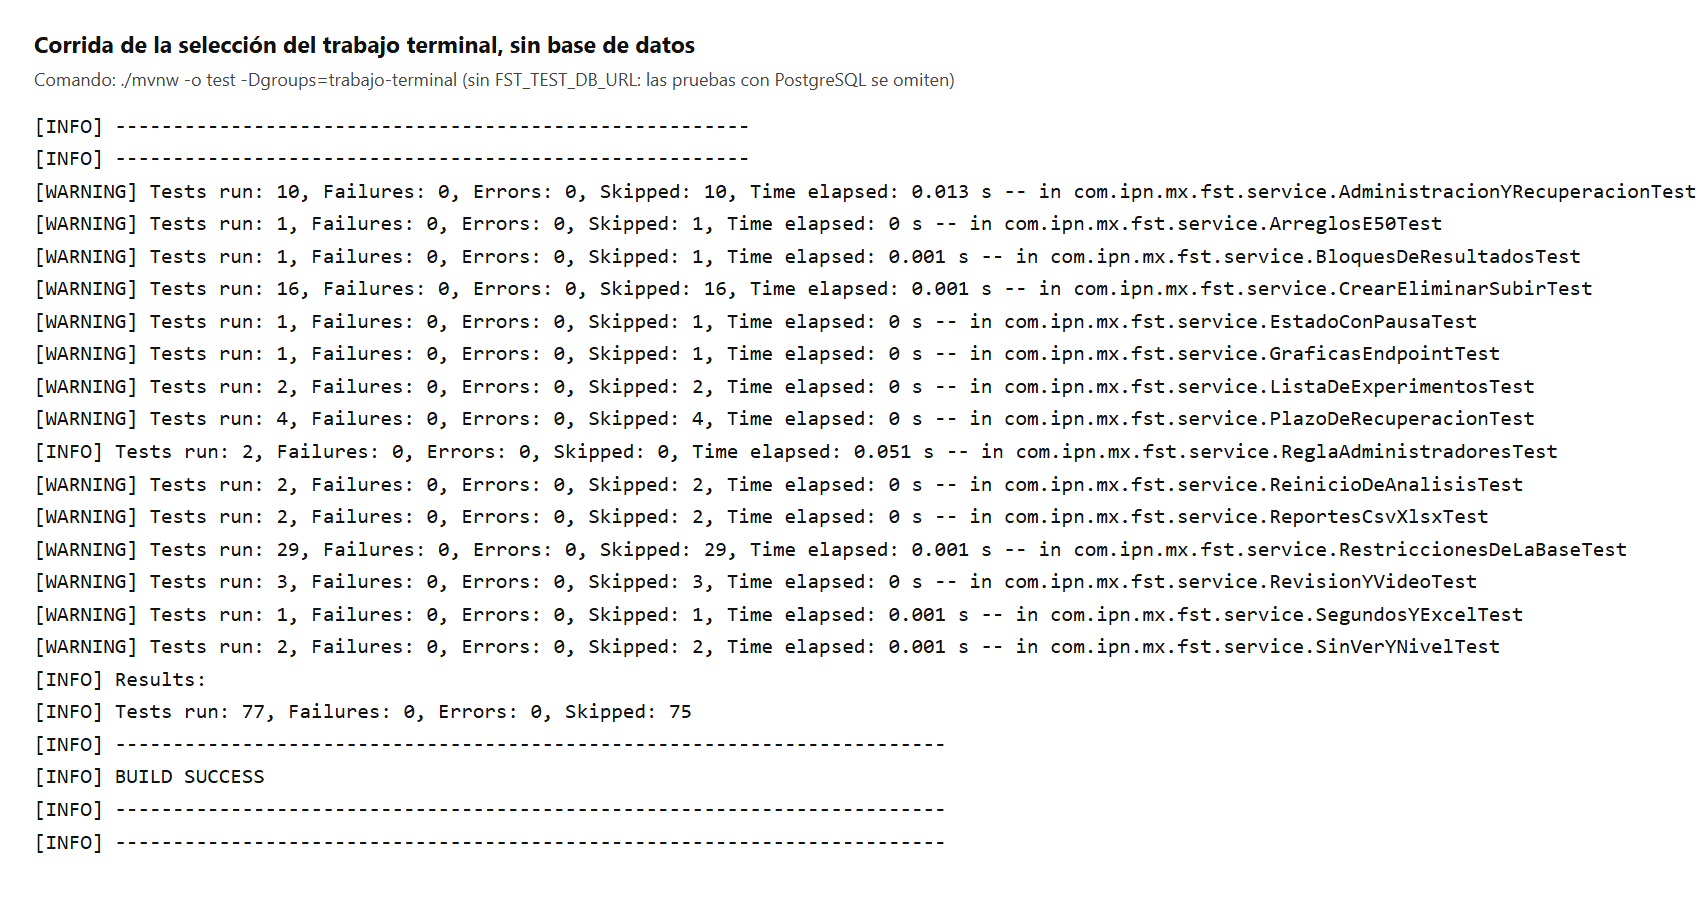
\includegraphics[width=\textheight, height=0.9\textwidth, keepaspectratio]{figures/pruebas/02_corrida_77_sin_base}
\caption{Salida de la corrida de la selección sin base de datos, reproducida como texto a partir del registro de Maven y de los reportes de las pruebas.}
\label{fig:pruebas_corrida_sin_base}
\end{sidewaysfigure}

\subsection{Plan de pruebas por tipo}

Cada prueba de la selección se clasificó una sola vez según su propósito principal. La
Tabla~\ref{tab:pruebas_tipos} describe los tipos, cuándo se aplican, qué validan y cuántas
de las 77 pruebas corresponden a cada uno. Setenta y cinco de las 77 corren contra la
aplicación completa y PostgreSQL reales; el tipo «integración» indica el propósito
principal de la prueba (que varias partes juntas dejen el sistema en el estado correcto),
no el entorno en que corre. La selección es solo del \textit{backend}, por lo que no
incluye un tipo «interfaz».

{\footnotesize\singlespacing
\begin{longtable}{|>{\raggedright}p{1.8cm}|>{\raggedright}p{2.8cm}|>{\raggedright}p{2.6cm}|>{\raggedright}p{4.5cm}|>{\raggedright\arraybackslash}p{1.2cm}|}
\caption{Tipos de prueba de la selección, con el número de pruebas de cada uno.
\label{tab:pruebas_tipos}}\\
\hline
\textbf{Tipo} & \textbf{Objetivo} & \textbf{Cuándo se aplica} & \textbf{Qué valida} & \textbf{Pruebas} \\
\hline
\endfirsthead
\hline
\textbf{Tipo} & \textbf{Objetivo} & \textbf{Cuándo se aplica} & \textbf{Qué valida} & \textbf{Pruebas} \\
\hline
\endhead
Funcional
& Comprobar que una función entrega el resultado que describe el requerimiento.
& Cada vez que se corre la selección, tras un cambio en la función.
& Que subir un video horizontal del Día~2 cree la tanda y deje el análisis en cola, y que el CSV del grupo traiga las columnas, las filas y los estadísticos.
& 20 \\
\hline
Validación de datos
& Comprobar que los datos válidos entran y los que están fuera de formato o de rango se rechazan.
& Tras un cambio en las reglas de formato o en el esquema de la base.
& Que un archivo que no es MP4 ni MOV o un video vertical se rechacen, y que la base rechace un segundo igual a 0 o a 301 y una duración de 0.
& 21 \\
\hline
Negativa (rechazo de lo no permitido)
& Comprobar que lo no permitido se rechaza y no deja cambios.
& Tras un cambio en las reglas de negocio.
& Que un nombre de experimento repetido dé conflicto, que no se elimine un experimento con un análisis procesando y que no se borre un experimento que tiene grupos.
& 20 \\
\hline
Seguridad
& Comprobar que solo se accede a lo que corresponde a cada cuenta.
& Tras un cambio en cuentas, sesión o permisos.
& Que un investigador reciba acceso denegado en todo el panel de administración, que con contraseña temporal cambiarla exija aceptar el aviso de privacidad y los términos, y que el enlace de recuperación sirva una sola vez.
& 12 \\
\hline
Integración
& Comprobar que varias partes juntas dejan el sistema en el estado correcto.
& Tras un cambio que toque más de una parte del sistema.
& Que al eliminar un experimento desaparezcan sus grupos, tandas y notificaciones; que de dos reinicios a la vez solo pase uno; que el candado de cuenta deje pasar la notificación del \textit{worker}; y que reiniciar deje el análisis en cola sin resultados ni archivos viejos.
& 4 \\
\hline
Rendimiento
& Medir el tiempo de respuesta bajo carga.
& Con el sistema armado.
& Ninguna de las 77 pruebas es de este tipo: la prueba de carga es manual y se describe aparte (sección~\ref{sec:pruebas_carga}).
& 0 \\
\hline
\textbf{Total}
& & & & \textbf{77} \\
\hline
\end{longtable}
}

\subsection{Pruebas por tema}

La Tabla~\ref{tab:pruebas_seleccion} agrupa las 77 pruebas por tema. Indica qué comprueba
cada grupo y qué requerimientos funcionales (RF) y no funcionales (RNF) del
capítulo~4 verifica. Las restricciones de la base de datos no verifican un requerimiento
directo: comprueban la integridad de los datos y se describen en la
sección~\ref{sec:pruebas_bd}.

{\footnotesize\singlespacing
\begin{longtable}{|>{\raggedright}p{2.7cm}|>{\raggedright}p{1.4cm}|>{\raggedright}p{6.0cm}|>{\raggedright\arraybackslash}p{3.0cm}|}
\caption{Pruebas seleccionadas del trabajo terminal, por tema.
\label{tab:pruebas_seleccion}}\\
\hline
\textbf{Tema} & \textbf{Pruebas} & \textbf{Qué comprueban} & \textbf{RF y RNF que verifican} \\
\hline
\endfirsthead
\hline
\textbf{Tema} & \textbf{Pruebas} & \textbf{Qué comprueban} & \textbf{RF y RNF que verifican} \\
\hline
\endhead
Cuentas, sesión y recuperación
& 11
& Que no se pueda quitar al único Administrador activo, ni desactivarlo, ni que se dé una contraseña temporal a sí mismo; que un investigador no entre a la administración; que con contraseña temporal solo se pueda cambiarla aceptando el aviso y los términos; que un correo o identificador repetido se rechace; que el enlace de recuperación sirva una sola vez y no sirva vencido.
& RF-03, 04, 05, 06 y 07; RNF-05. \\
\hline
Experimentos y carga de video
& 18
& Que se pueda crear y eliminar un experimento con las reglas de quién puede hacerlo y de cuándo no (si hay un análisis en curso o en pausa); que se filtre la lista por estado y aparezca el aviso de vencimiento a 7 días; que la subida de video rechace un archivo que no es MP4 ni MOV y un video vertical, y que acepte uno horizontal y cree su tanda, con el Día~1 sin análisis y un solo video por día en cada tanda.
& RF-08, 09, 10, 11, 12, 23, 24, 27 y 30; RNF-04. \\
\hline
Pausa
& 1
& Que el estado de un análisis en pausa traiga el cilindro, el segundo y el plazo que queda.
& RF-15. \\
\hline
Plazo del enlace de recuperación
& 4
& Que el enlace dure exactamente lo configurado (60 minutos), sirva dentro de su plazo y una sola vez, siga sirviendo a los 59 minutos y ya no sirva a los 62.
& RF-03. \\
\hline
Resultados y reportes
& 6
& Que los bloques de cada espécimen, los totales (con las cinco claves, que suman 100\,\%), la comparación entre grupos, el CSV, el XLSX y el Excel del experimento traigan las columnas, los datos y los estadísticos esperados.
& RF-18, 19, 20, 21, 22 y 31. \\
\hline
Revisión segundo a segundo
& 5
& Que el video se entregue con un permiso temporal y no con la sesión; que se guarden solo los segundos corregidos; que la corrección ajuste el nivel de clasificación; y que reiniciar un análisis lo deje en cola sin resultados, reportes ni archivos anteriores.
& RF-32; RNF-04. \\
\hline
Notificaciones y concurrencia
& 3
& Que el contador de notificaciones no leídas cuente todas las de la cuenta; que de dos reinicios simultáneos de un análisis solo pase uno; y que una notificación del \textit{worker} no se bloquee mientras otro cambio de cuenta está en curso.
& RF-32 y RF-33. \\
\hline
Restricciones de la base de datos
& 29
& Que la base acepte los datos válidos y rechace los que están fuera de rango, fuera de un dominio de valores cerrados, repetidos o que dejarían filas huérfanas (sección~\ref{sec:pruebas_bd}).
& Ninguno directo: integridad de los datos. \\
\hline
\textbf{Total}
& \textbf{77}
& &  \\
\hline
\end{longtable}
}

Las Figuras~\ref{fig:pruebas_experimentos}, \ref{fig:pruebas_cuentas} y
\ref{fig:pruebas_resultados} muestran el resultado de cada prueba, con su tiempo. Las
capturas agrupan las pruebas por clase de prueba y no por tema, por lo que su reparto
(18, 16 y 14 pruebas) no coincide con el de la Tabla~\ref{tab:pruebas_seleccion}; junto con
las 29 de la Figura~\ref{fig:pruebas_restricciones} suman las mismas 77.

\begin{sidewaysfigure}[p]
\centering
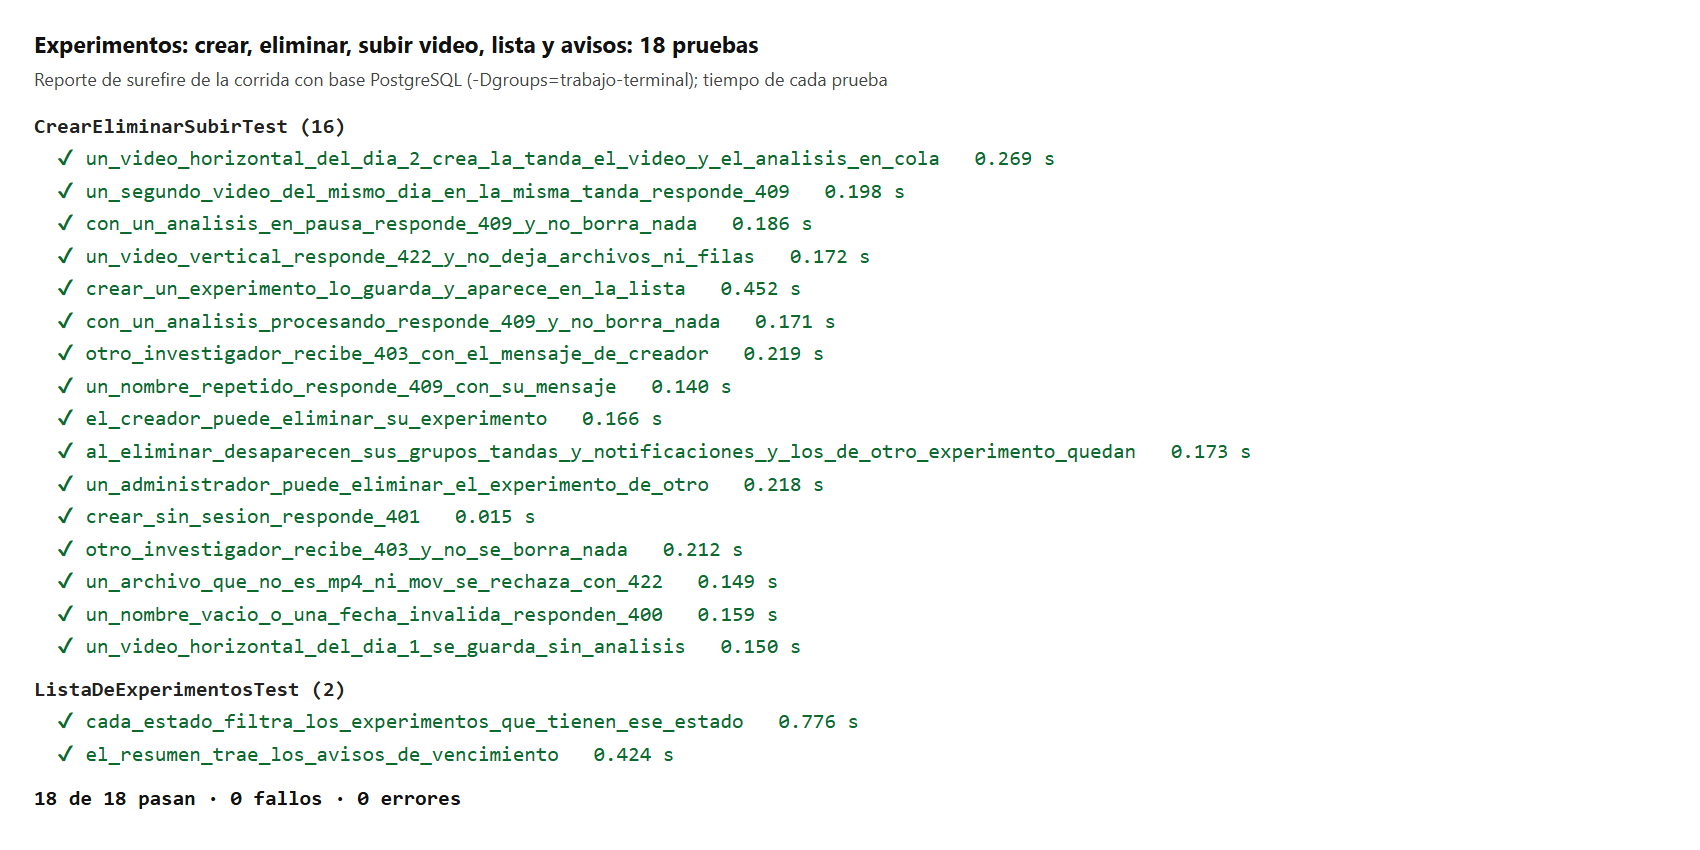
\includegraphics[width=\textheight, height=0.9\textwidth, keepaspectratio]{figures/pruebas/04_experimentos_crear_eliminar_subir}
\caption{Salida de la corrida de las pruebas de experimentos (crear, eliminar, subir video, filtro por estado y aviso de vencimiento), reproducida como texto a partir del registro de Maven y de los reportes de las pruebas.}
\label{fig:pruebas_experimentos}
\end{sidewaysfigure}

\begin{sidewaysfigure}[p]
\centering
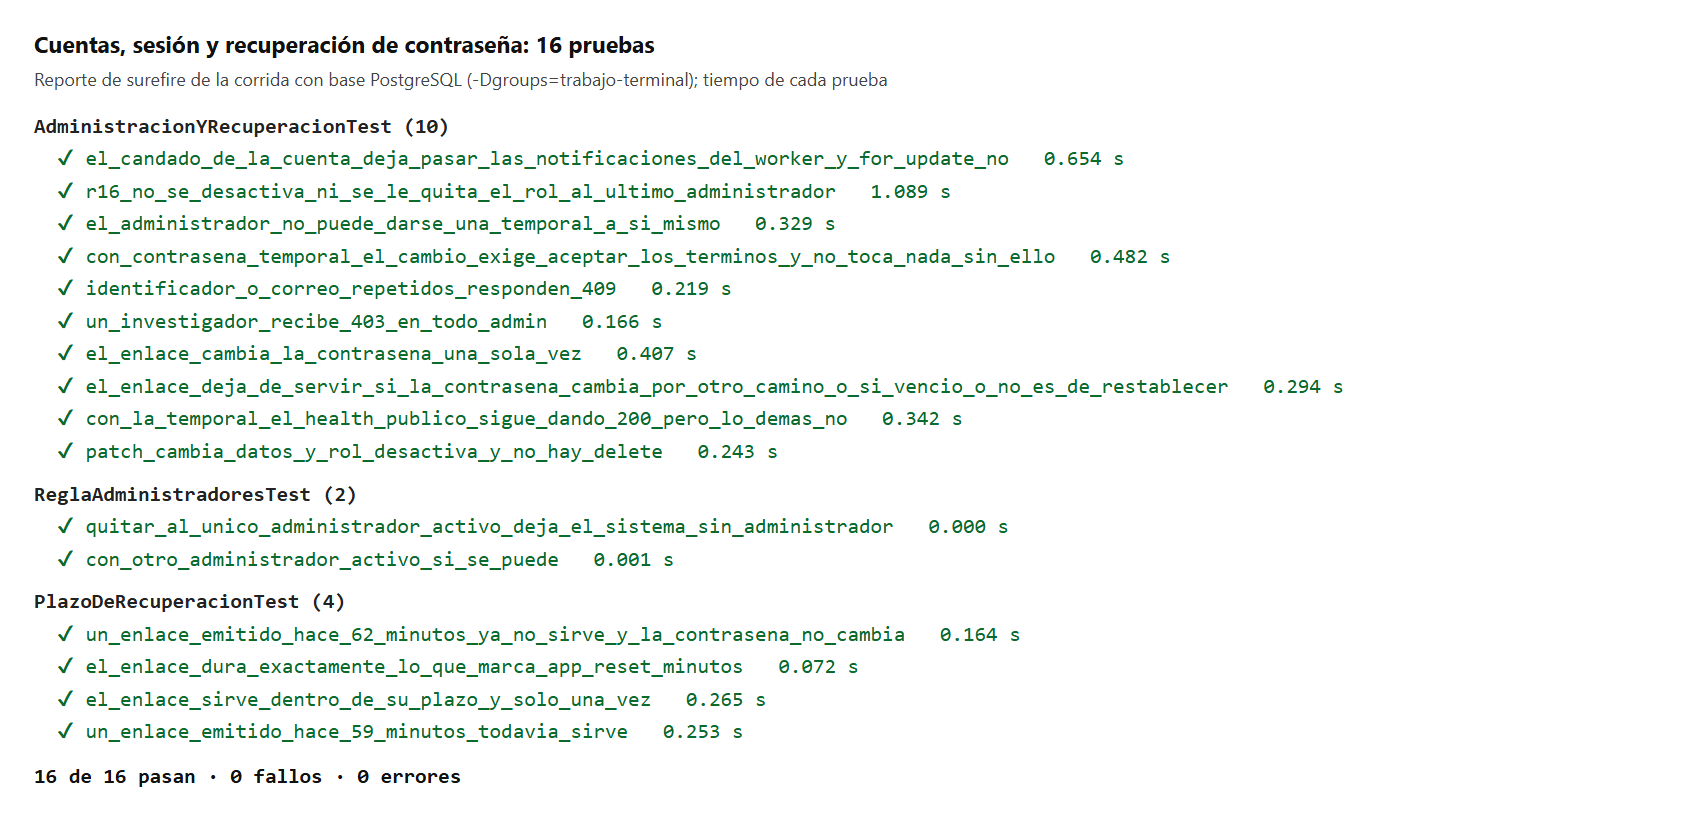
\includegraphics[width=\textheight, height=0.9\textwidth, keepaspectratio]{figures/pruebas/05_cuentas_sesion_y_recuperacion}
\caption{Salida de la corrida de las pruebas de cuentas, sesión y recuperación de contraseña, reproducida como texto a partir del registro de Maven y de los reportes de las pruebas.}
\label{fig:pruebas_cuentas}
\end{sidewaysfigure}

\begin{sidewaysfigure}[p]
\centering
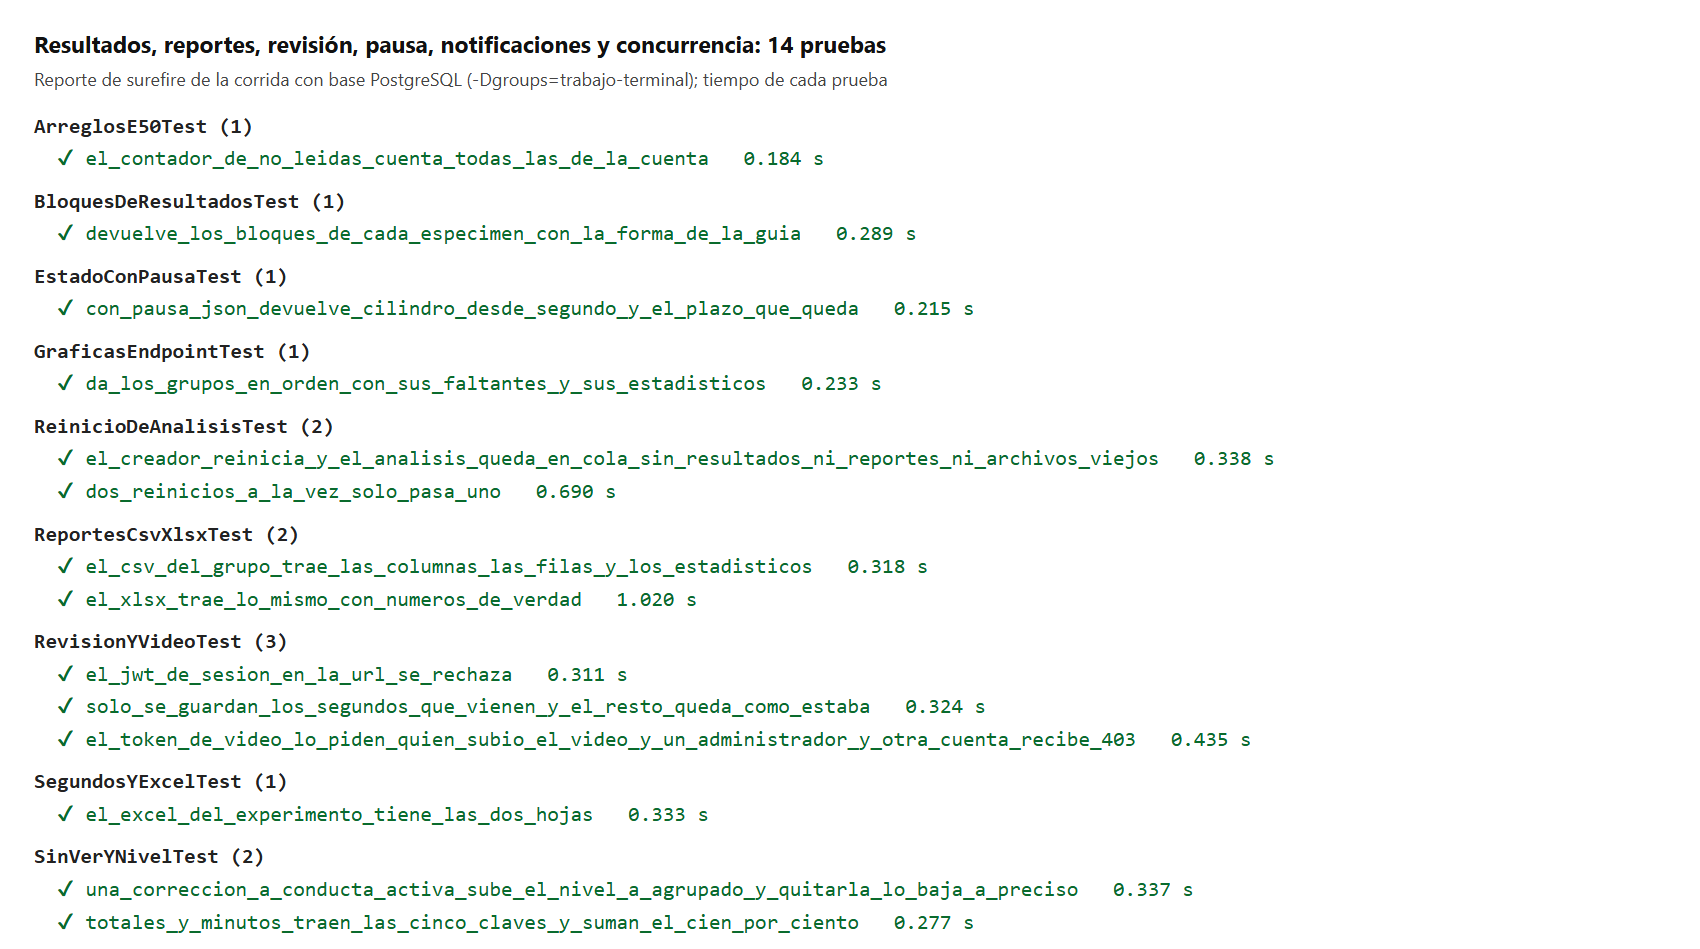
\includegraphics[width=\textheight, height=0.9\textwidth, keepaspectratio]{figures/pruebas/06_resultados_revision_y_demas}
\caption{Salida de la corrida de las pruebas de resultados y reportes, revisión segundo a segundo, pausa, notificaciones y concurrencia, reproducida como texto a partir del registro de Maven y de los reportes de las pruebas.}
\label{fig:pruebas_resultados}
\end{sidewaysfigure}

\FloatBarrier

% ============================================================
\section{Restricciones de la base de datos}
\label{sec:pruebas_bd}

El esquema físico (Figura~\ref{fig:er} y apéndice~\ref{ap:diccionario}) declara reglas
que la base de datos hace cumplir por sí misma, sin depender de la aplicación. Las 29 pruebas
de este grupo intentan insertar, repetir o borrar datos directamente en la base y
comprueban que responda como el esquema establece. La Figura~\ref{fig:pruebas_restricciones}
muestra el resultado de cada una. Se agrupan en cinco tipos:

\begin{itemize}
  \item \textbf{Controles de que lo válido sí entra.} Una cadena completa y válida de
        registros se inserta sin error; las tandas de dos y de cuatro cilindros son
        válidas; los segundos 1 y 300 son válidos; un video con duración positiva es
        válido; y un análisis con error y diagnóstico es válido. Evitan que una restricción
        demasiado estricta rechace datos legítimos.
  \item \textbf{Rechazo de valores fuera de rango.} La base rechaza una tanda de uno o de
        cinco cilindros, un ordinal de tanda igual a cero, un número de cilindro de espécimen
        igual a cero o a cinco, un segundo igual a cero o a 301, una duración de video igual a
        cero o negativa, y un diagnóstico en un análisis cuyo estado no es de error.
  \item \textbf{Dominios de valores cerrados.} La base rechaza un tipo de grupo, un estado
        de análisis y una conducta que no estén en su lista de valores permitidos.
  \item \textbf{Valores únicos.} La base rechaza un correo de usuario repetido, un
        ordinal repetido dentro del mismo grupo, una sesión repetida en la misma tanda, un
        número de cilindro repetido en la misma tanda, un nombre de experimento repetido y un
        segundo análisis del mismo video.
  \item \textbf{Llaves foráneas.} La base impide borrar un usuario que tiene experimentos,
        un experimento que tiene grupos, un grupo que tiene tandas, una tanda que tiene videos
        y un video que tiene análisis; es decir, no borra lo que otra tabla todavía usa.
\end{itemize}

Estas pruebas no cubren todo lo que el esquema declara. \textbf{No existe prueba} de la
regla de actualización de las llaves foráneas (que tampoco actualiza en cascada), de los
valores por defecto, de los índices ni de las migraciones. Esos elementos están declarados y
la base los hace cumplir, pero ninguna prueba de la selección los verifica.

\begin{sidewaysfigure}[p]
\centering
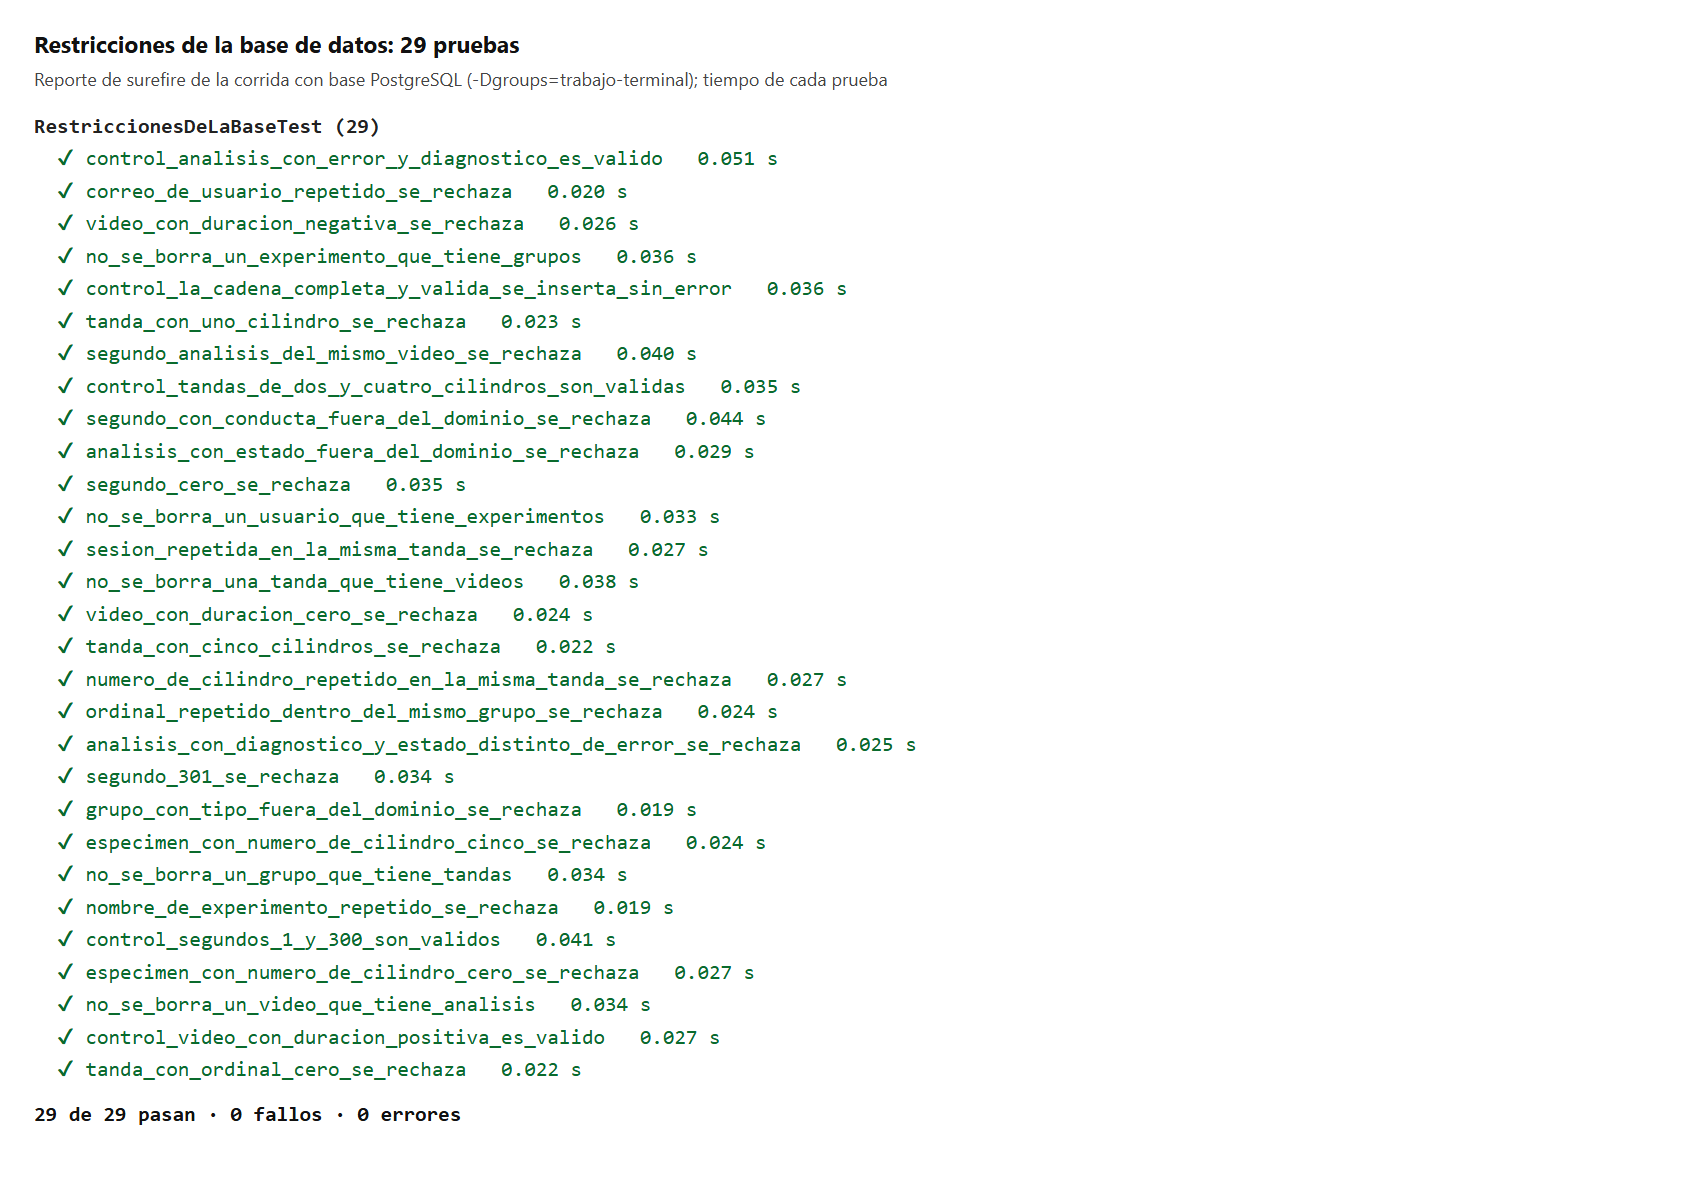
\includegraphics[width=\textheight, height=0.9\textwidth, keepaspectratio]{figures/pruebas/03_restricciones_de_la_base}
\caption{Salida de la corrida de las pruebas de restricciones de la base de datos, reproducida como texto a partir del registro de Maven y de los reportes de las pruebas.}
\label{fig:pruebas_restricciones}
\end{sidewaysfigure}

\FloatBarrier

% ============================================================
\section{Prueba de carga y despliegue}
\label{sec:pruebas_carga}

La prueba de carga comprueba que el sistema responda en menos de 3~s (RNF-01) cuando
trabajan cuatro usuarios a la vez (RNF-13). Se hizo con un programa propio que abre una
sesión por cliente, repite las consultas habituales del sistema y mide el tiempo de cada
respuesta. Se hicieron dos corridas, que resume la Tabla~\ref{tab:pruebas_carga}.

La prueba de carga y el despliegue son verificaciones manuales del sistema completo, no
pruebas automáticas, y no forman parte de las 77 pruebas seleccionadas. La corrida B se hizo
sobre la configuración de despliegue del sistema, con el servidor web nginx.

En esta sección se usa el \textbf{percentil 95}, que es el tiempo por debajo del cual
respondió el 95\,\% de las peticiones: describe lo que vive casi cualquier usuario sin que el
extremo más lento lo distorsione.

{\footnotesize\singlespacing
\begin{longtable}{|>{\raggedright}p{2.8cm}|>{\raggedright}p{5.4cm}|>{\raggedright\arraybackslash}p{5.2cm}|}
\caption{Corridas de la prueba de carga con cuatro sesiones.
\label{tab:pruebas_carga}}\\
\hline
\textbf{Concepto} & \textbf{Corrida A} & \textbf{Corrida B} \\
\hline
\endfirsthead
\hline
\textbf{Concepto} & \textbf{Corrida A} & \textbf{Corrida B} \\
\hline
\endhead
Clientes
& 4, cada uno con su propia sesión.
& 4 cuentas distintas. \\
\hline
Rutas
& Inicio de sesión, lista, detalle, estado, resultados, minutos, bloques, grupos, CSV y XLSX.
& Consultas y revisión, incluida la primera generación del XLSX. \\
\hline
Peticiones
& 25 rondas sincronizadas; el total no se registró.
& 1\,474, durante 120~s en bucle. \\
\hline
Errores
& Ninguno: todas respondieron con éxito.
& Ninguno. \\
\hline
Percentil 95
& El mayor por ruta fue 0.086~s.
& 0.041~s para todas las peticiones. \\
\hline
Máximo
& 0.888~s, en la primera ronda, con la máquina virtual de Java sin calentar.
& 0.962~s, en la primera generación del XLSX. \\
\hline
\end{longtable}
}

\subsection{Resultado}

En ambas corridas todas las peticiones respondieron con éxito y el tiempo máximo quedó muy
por debajo de los 3~s de RNF-01. El sistema atendió sin errores a cuatro cuentas trabajando a la vez, que
es el número que fija RNF-13. La prueba cumple ambos requerimientos con mucho margen.

\subsection{Límites}

\begin{itemize}
  \item Se hizo con el \textit{worker} sin procesar nada. No se probó con un video real en
        análisis, por la memoria que se necesitaría: la máquina de pruebas tiene 15.7~GB y
        el análisis puede ocupar hasta 3.5~GB. Por eso la prueba no incluye la condición de
        RNF-13 que pide, además de las cuatro sesiones, al menos un análisis en cola.
  \item No incluye la subida de videos ni la primera generación del reporte en PDF.
  \item Solo se registraron la mediana, el percentil 95 y el máximo, no el promedio.
\end{itemize}

% ============================================================
\section{Verificación del sistema completo con un video real}
\label{sec:pruebas_real}

Las pruebas automáticas de las secciones anteriores verifican el \textit{backend}, pero ninguna
ejecuta el sistema completo. Para comprobar que las partes funcionan juntas se hizo una
verificación manual. Se armó el sistema completo en un montaje de prueba aparte, con la
interfaz, el servidor web, la API, la base de datos PostgreSQL, el \textit{worker} y el modelo,
construido con las imágenes de la versión actual del código. Por la API se subió el video de
una sesión del Día~2 de la prueba de nado forzado, de 5 minutos (301~s, resolución
$1920 \times 1080$). El \textit{worker} lo analizó en unos 9 minutos, con 4 especímenes y los
300~s del análisis. Las figuras de esta sección son capturas de la interfaz con ese resultado
real: no son del modo de ejemplo. Las cuentas que aparecen son cuentas de prueba.

Con ese análisis se comprobaron además las cuatro descargas del sistema. El reporte en PDF del
experimento salió con 3 páginas y marcadores. El CSV de la tanda trajo 24 filas de datos, más
la media, la desviación estándar, la varianza y la revisión. El XLSX de la tanda trajo la hoja
«Resultados» con 25 filas y 9 columnas. El Excel del experimento trajo las hojas «Resultados» y
«Segundo a segundo», esta última con 1201 filas y 11 columnas.

Esta verificación muestra que el sistema procesa un video real de principio a fin. No mide el
desempeño del clasificador. Además, el experimento tiene un solo grupo (Control) y una sola
tanda, por lo que la comparación entre grupos solo muestra el Control.

\subsection{Análisis en curso}

La Figura~\ref{fig:pruebas_real_progreso} muestra la pantalla del análisis mientras corre: el
preprocesamiento y la localización de los cilindros ya terminaron, la clasificación va en curso y la
cola indica que hay un análisis procesando.

\begin{figure}[tbp]
\centering
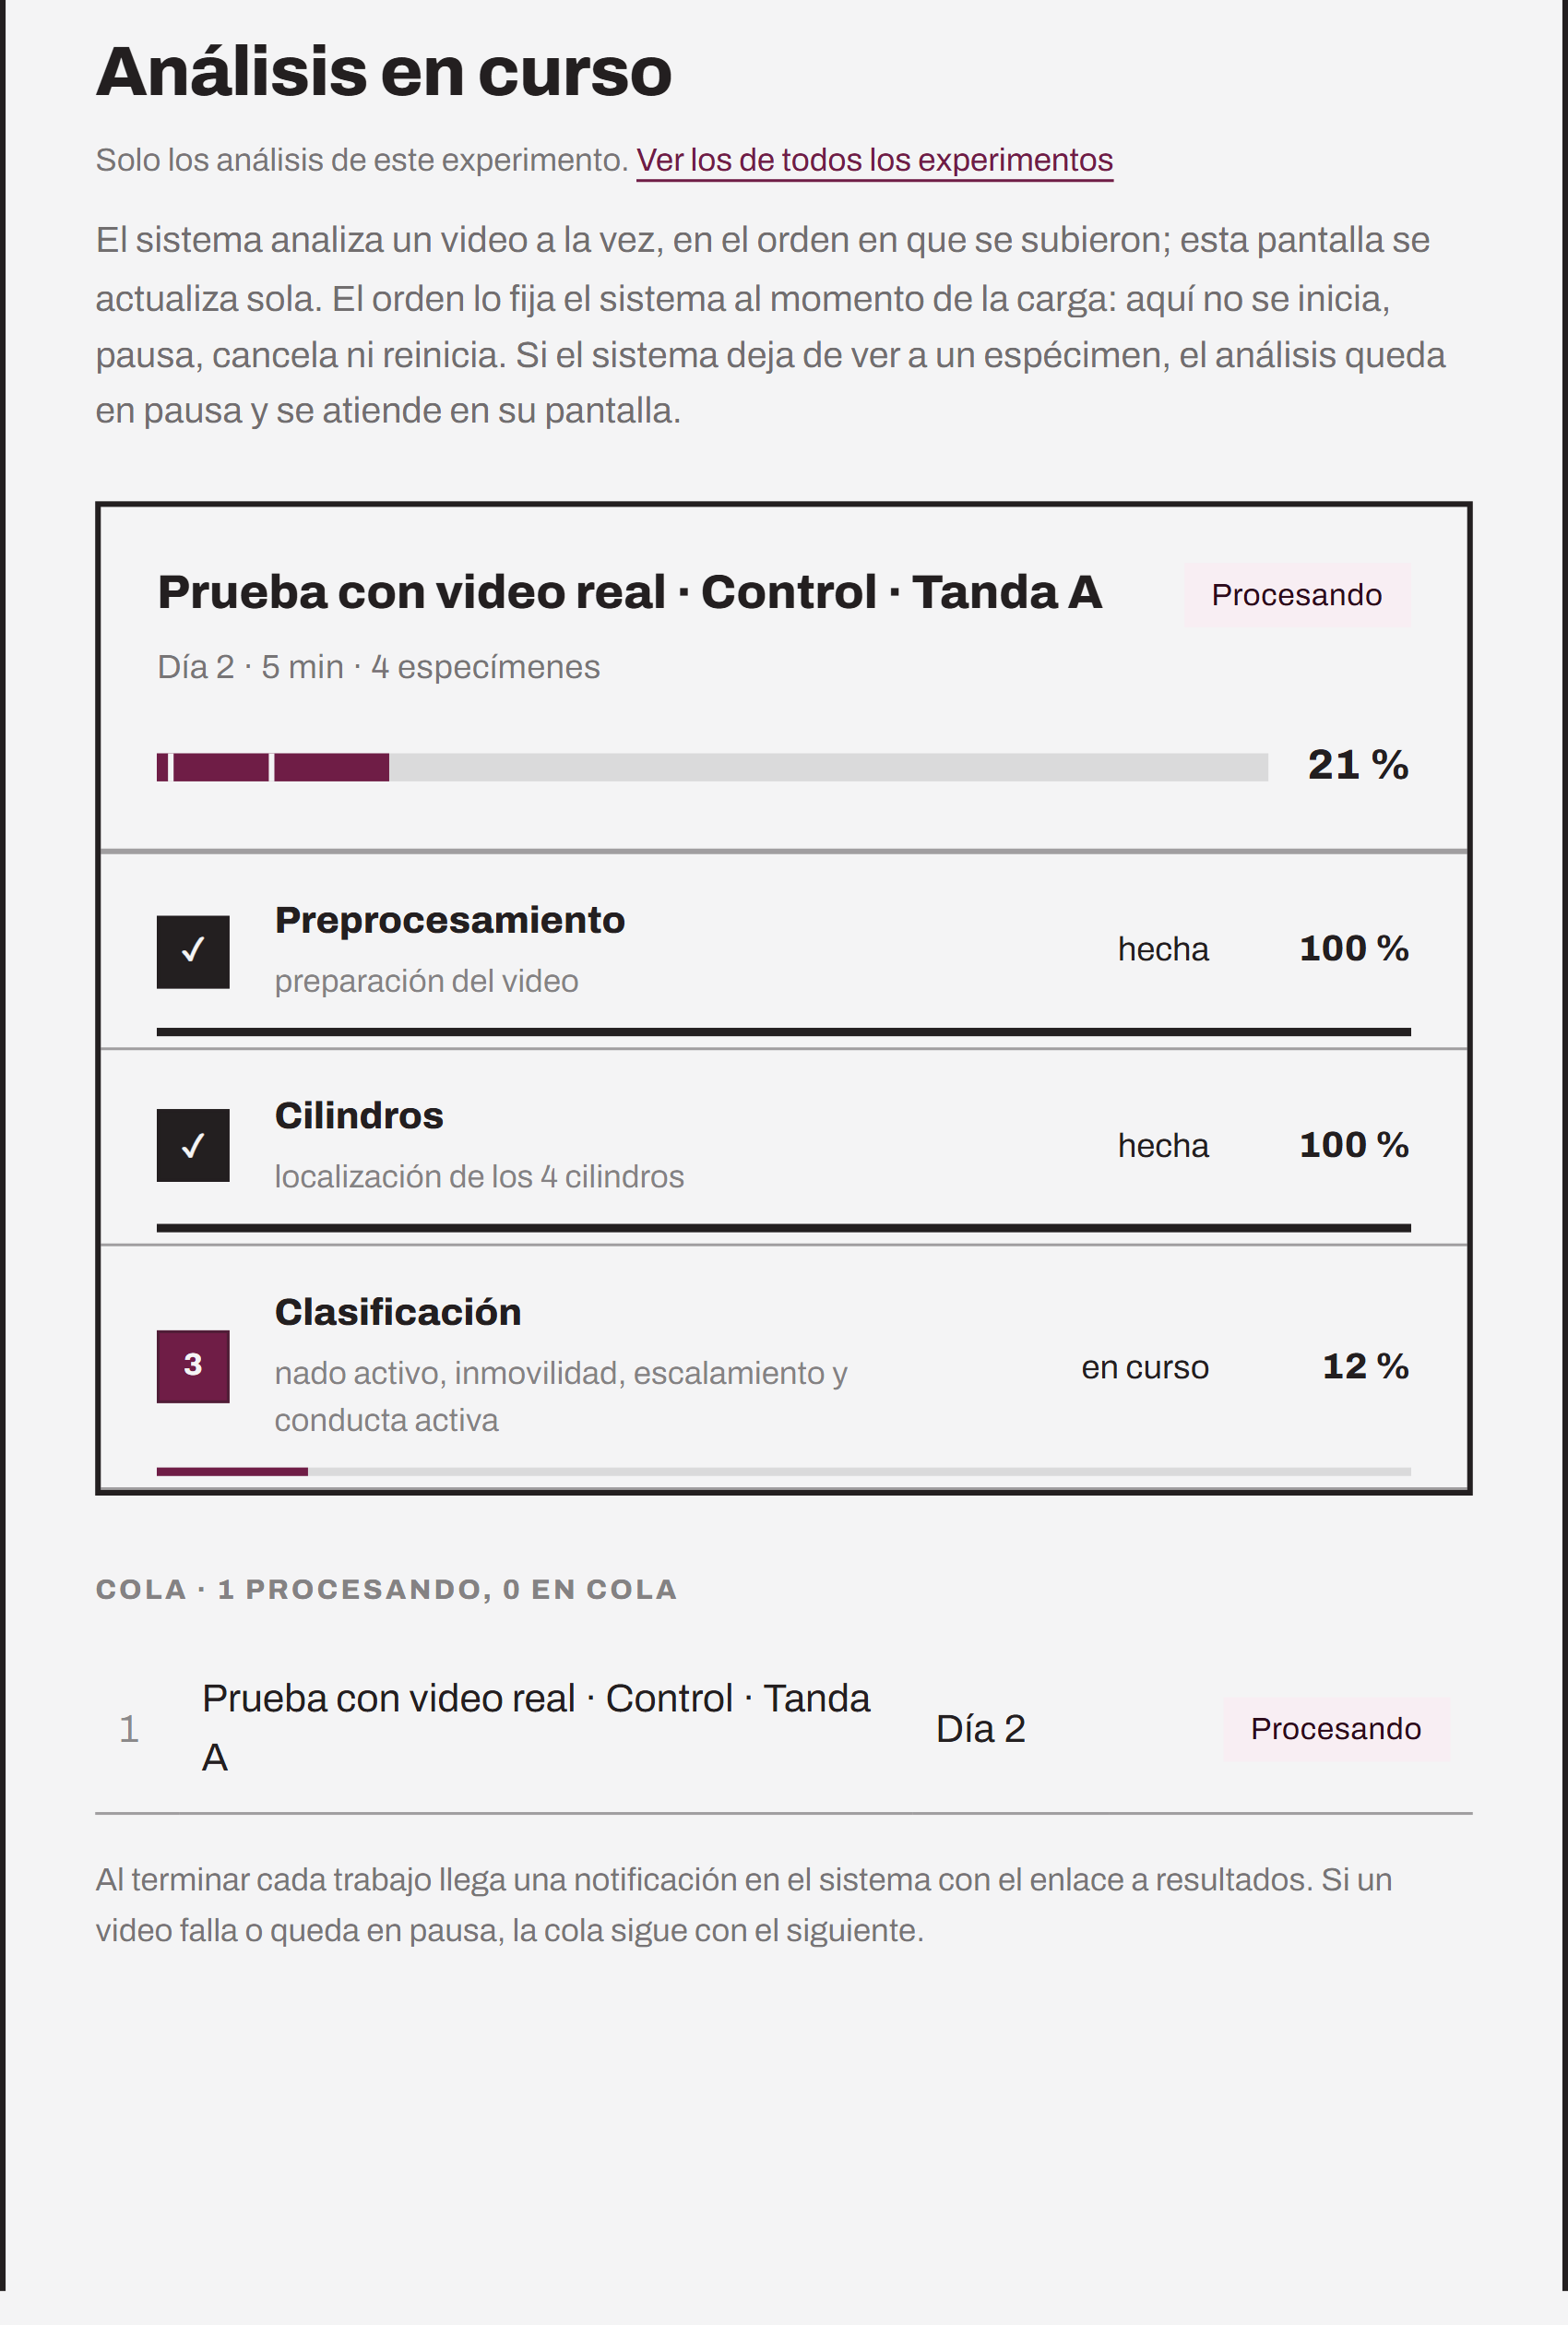
\includegraphics[width=0.75\textwidth]{figures/pruebas/30_real_progreso_del_analisis}
\caption{Captura de la interfaz con el sistema completo y un video real: análisis en curso, con el preprocesamiento y los cilindros hechos y la clasificación en curso.}
\label{fig:pruebas_real_progreso}
\end{figure}

\FloatBarrier

\subsection{Resultados}

La Figura~\ref{fig:pruebas_real_resumen} muestra el resumen de resultados del experimento una vez
terminado el análisis. Las Figuras~\ref{fig:pruebas_real_g1} a \ref{fig:pruebas_real_g6} muestran
las seis gráficas de la galería de resultados con los datos de este análisis.

\begin{figure}[tbp]
\centering
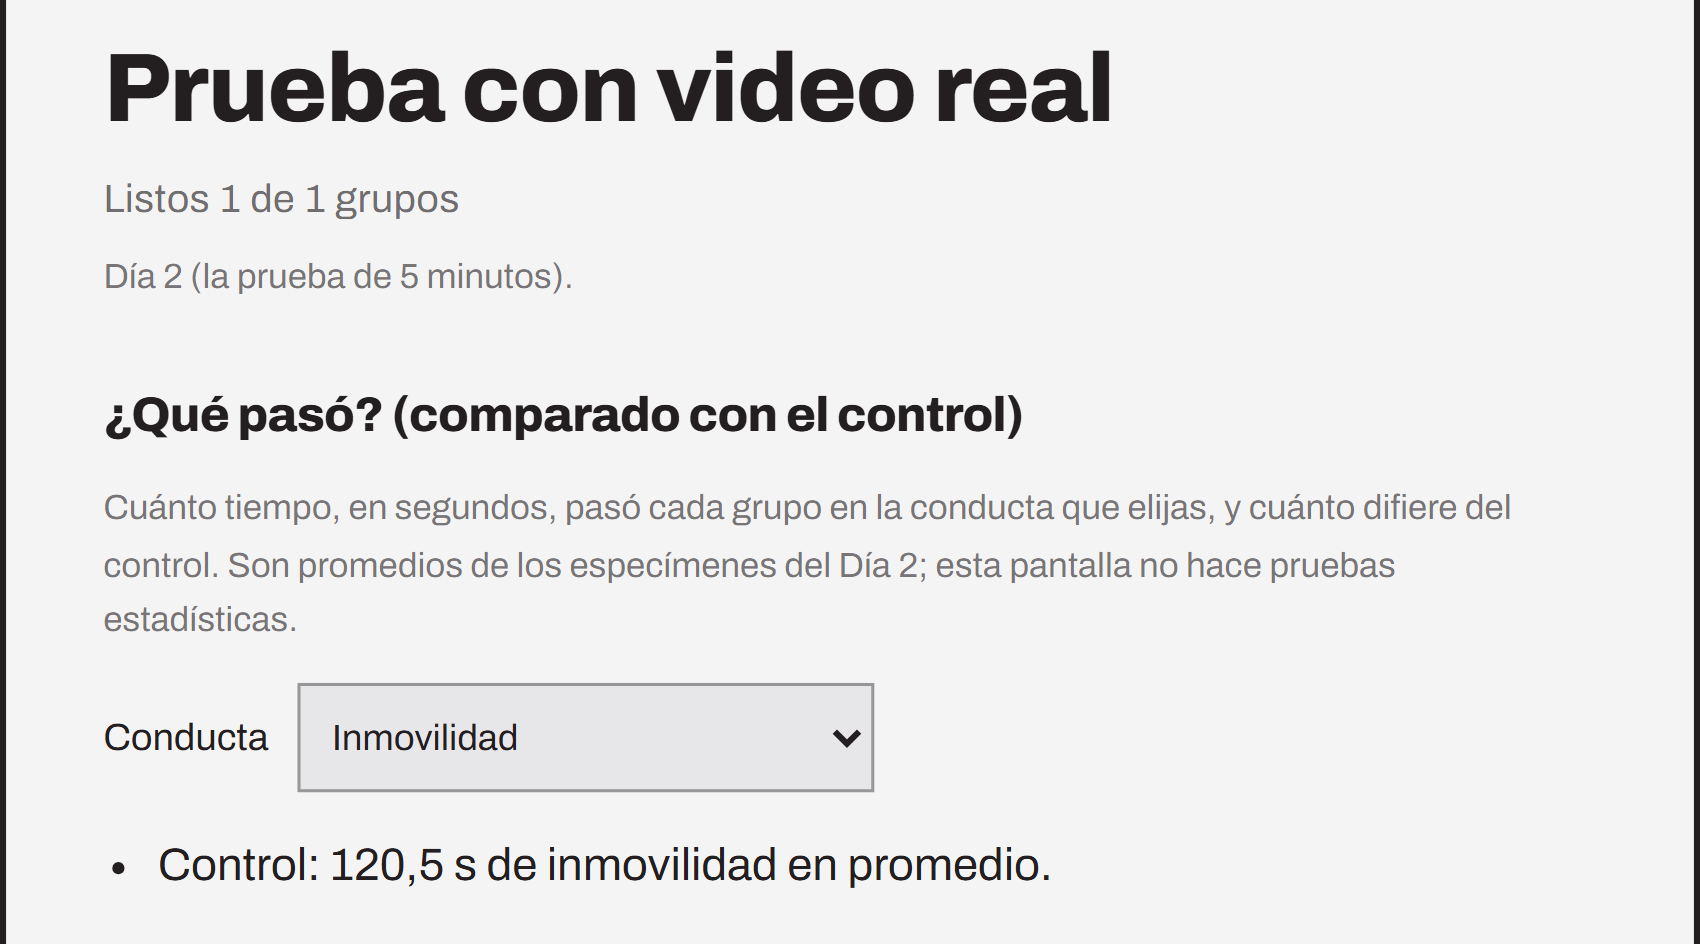
\includegraphics[width=0.75\textwidth]{figures/pruebas/31_real_resumen_de_resultados}
\caption{Captura de la interfaz con el sistema completo y un video real: resumen de resultados del experimento.}
\label{fig:pruebas_real_resumen}
\end{figure}

\begin{figure}[tbp]
\centering
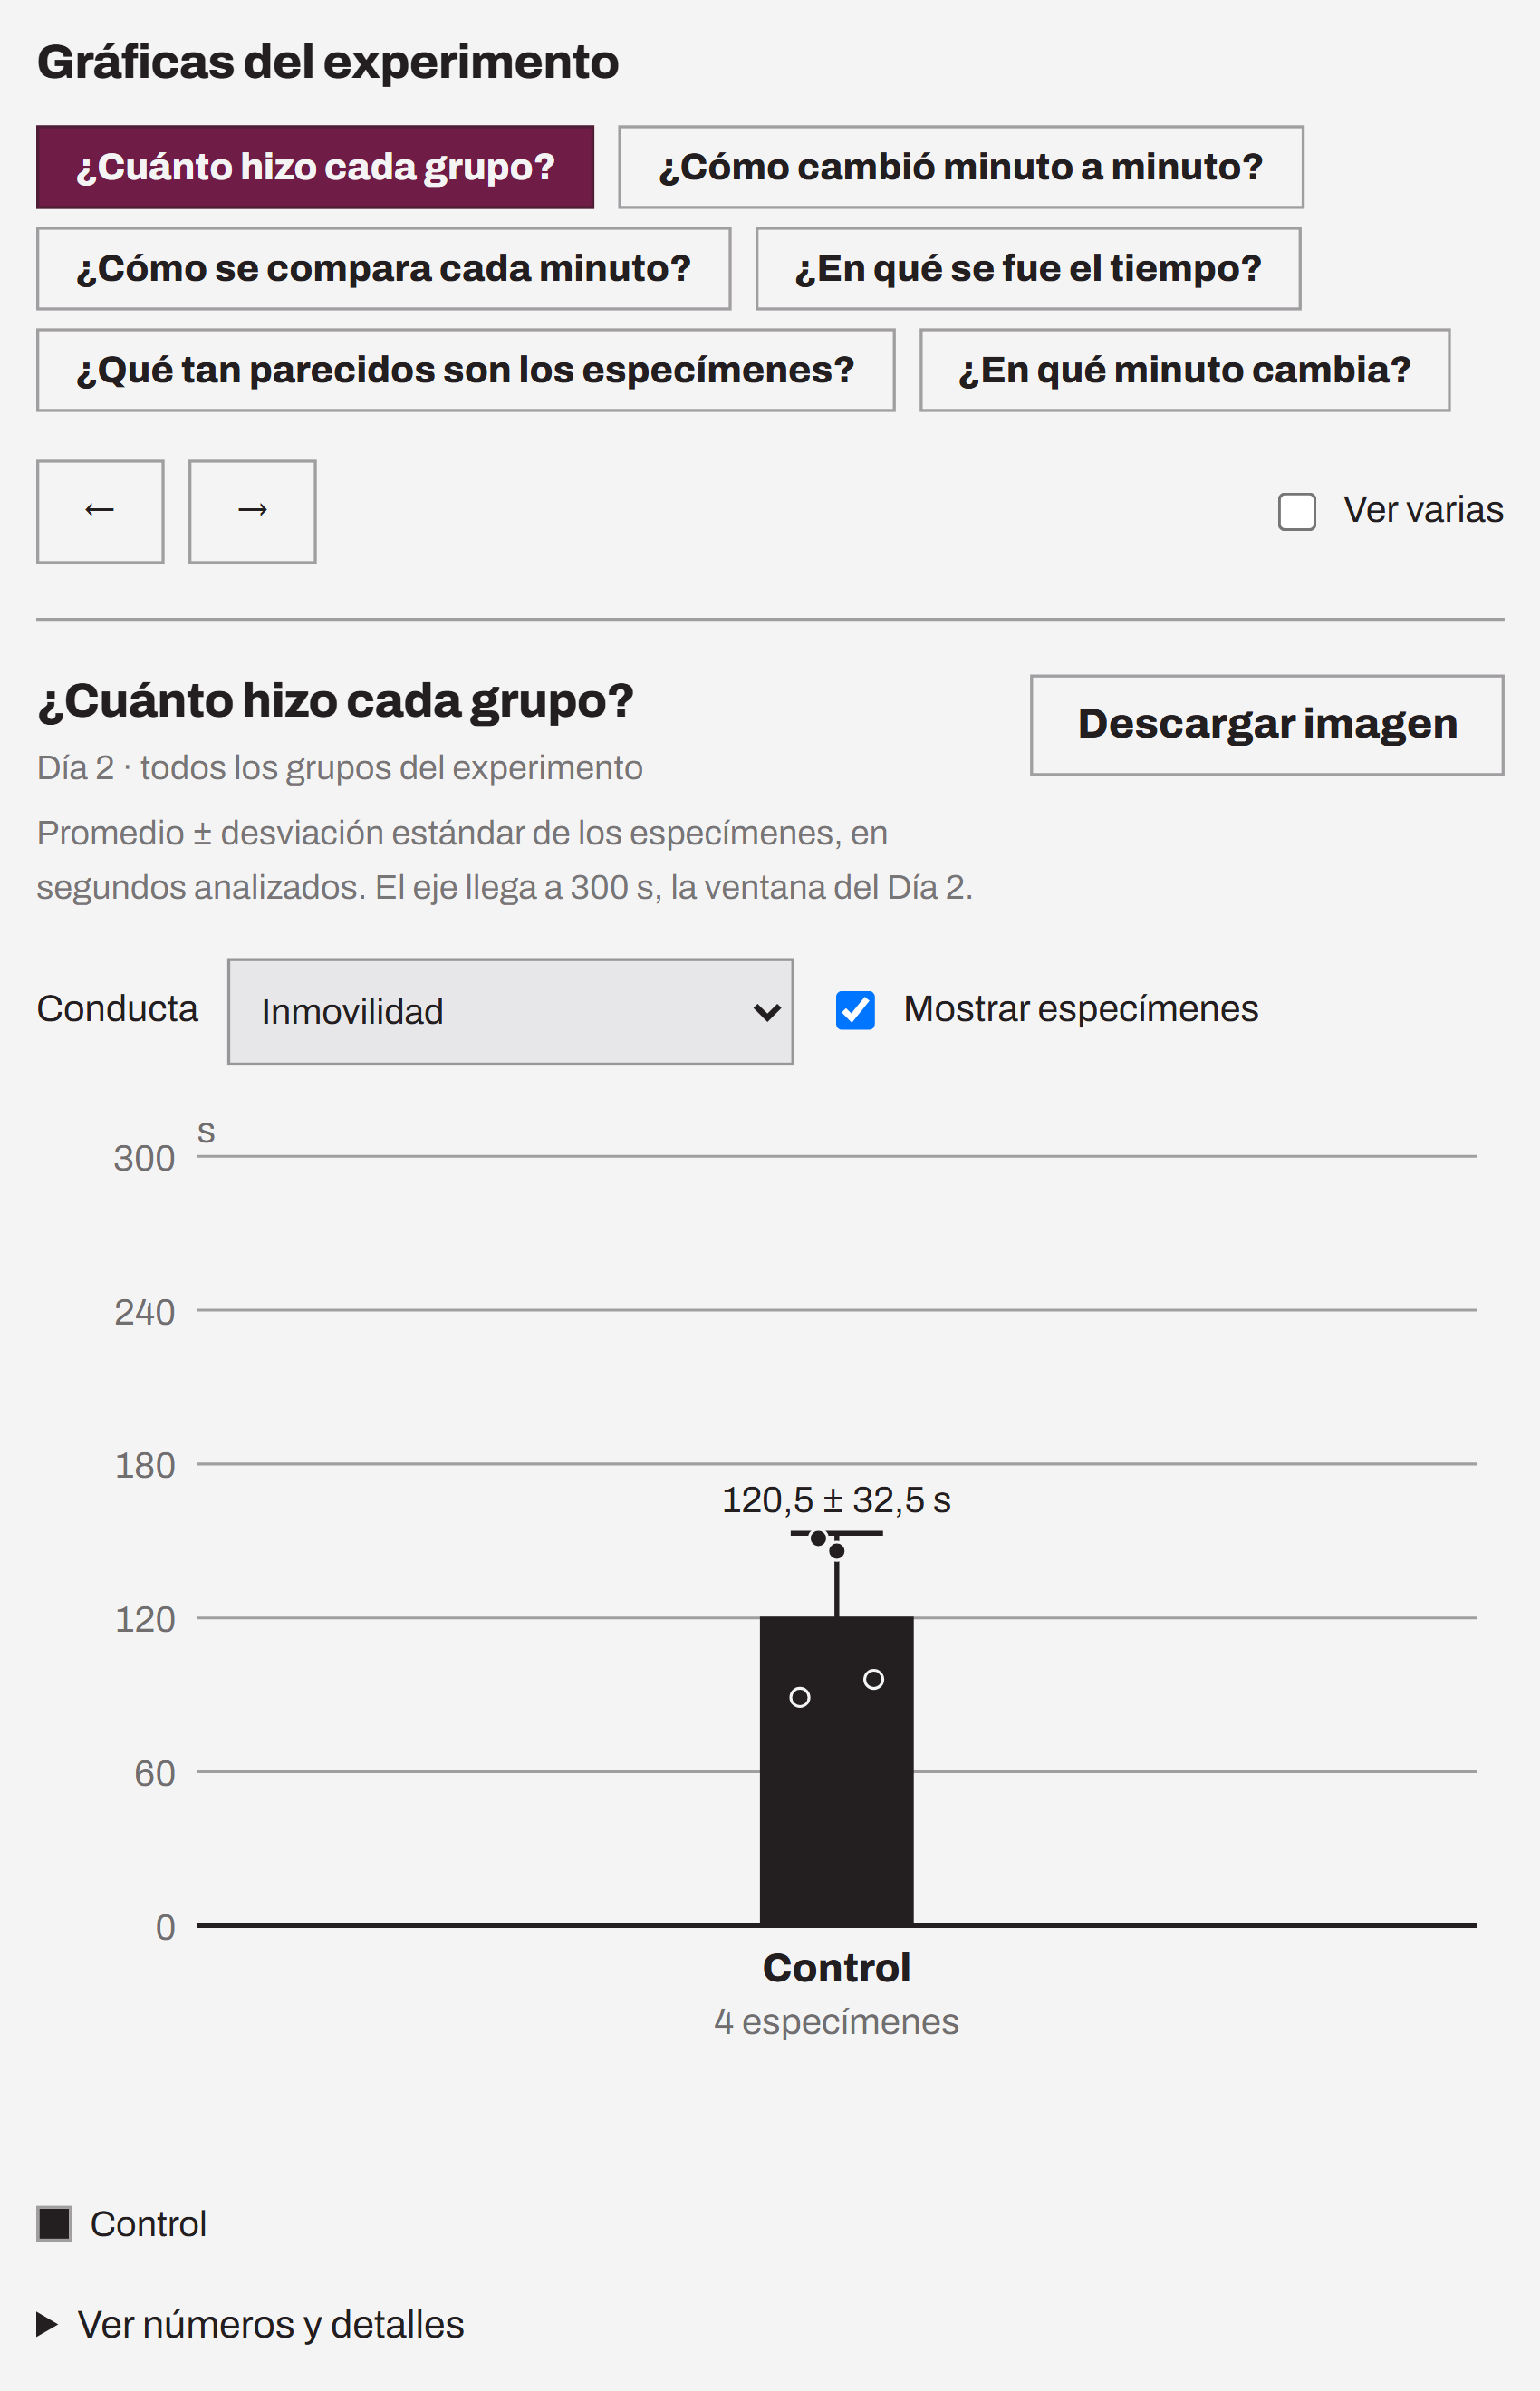
\includegraphics[width=0.7\textwidth]{figures/pruebas/32_real_grafica_barras_por_grupo}
\caption{Captura de la interfaz con el sistema completo y un video real: gráfica de barras por grupo.}
\label{fig:pruebas_real_g1}
\end{figure}

\begin{figure}[tbp]
\centering
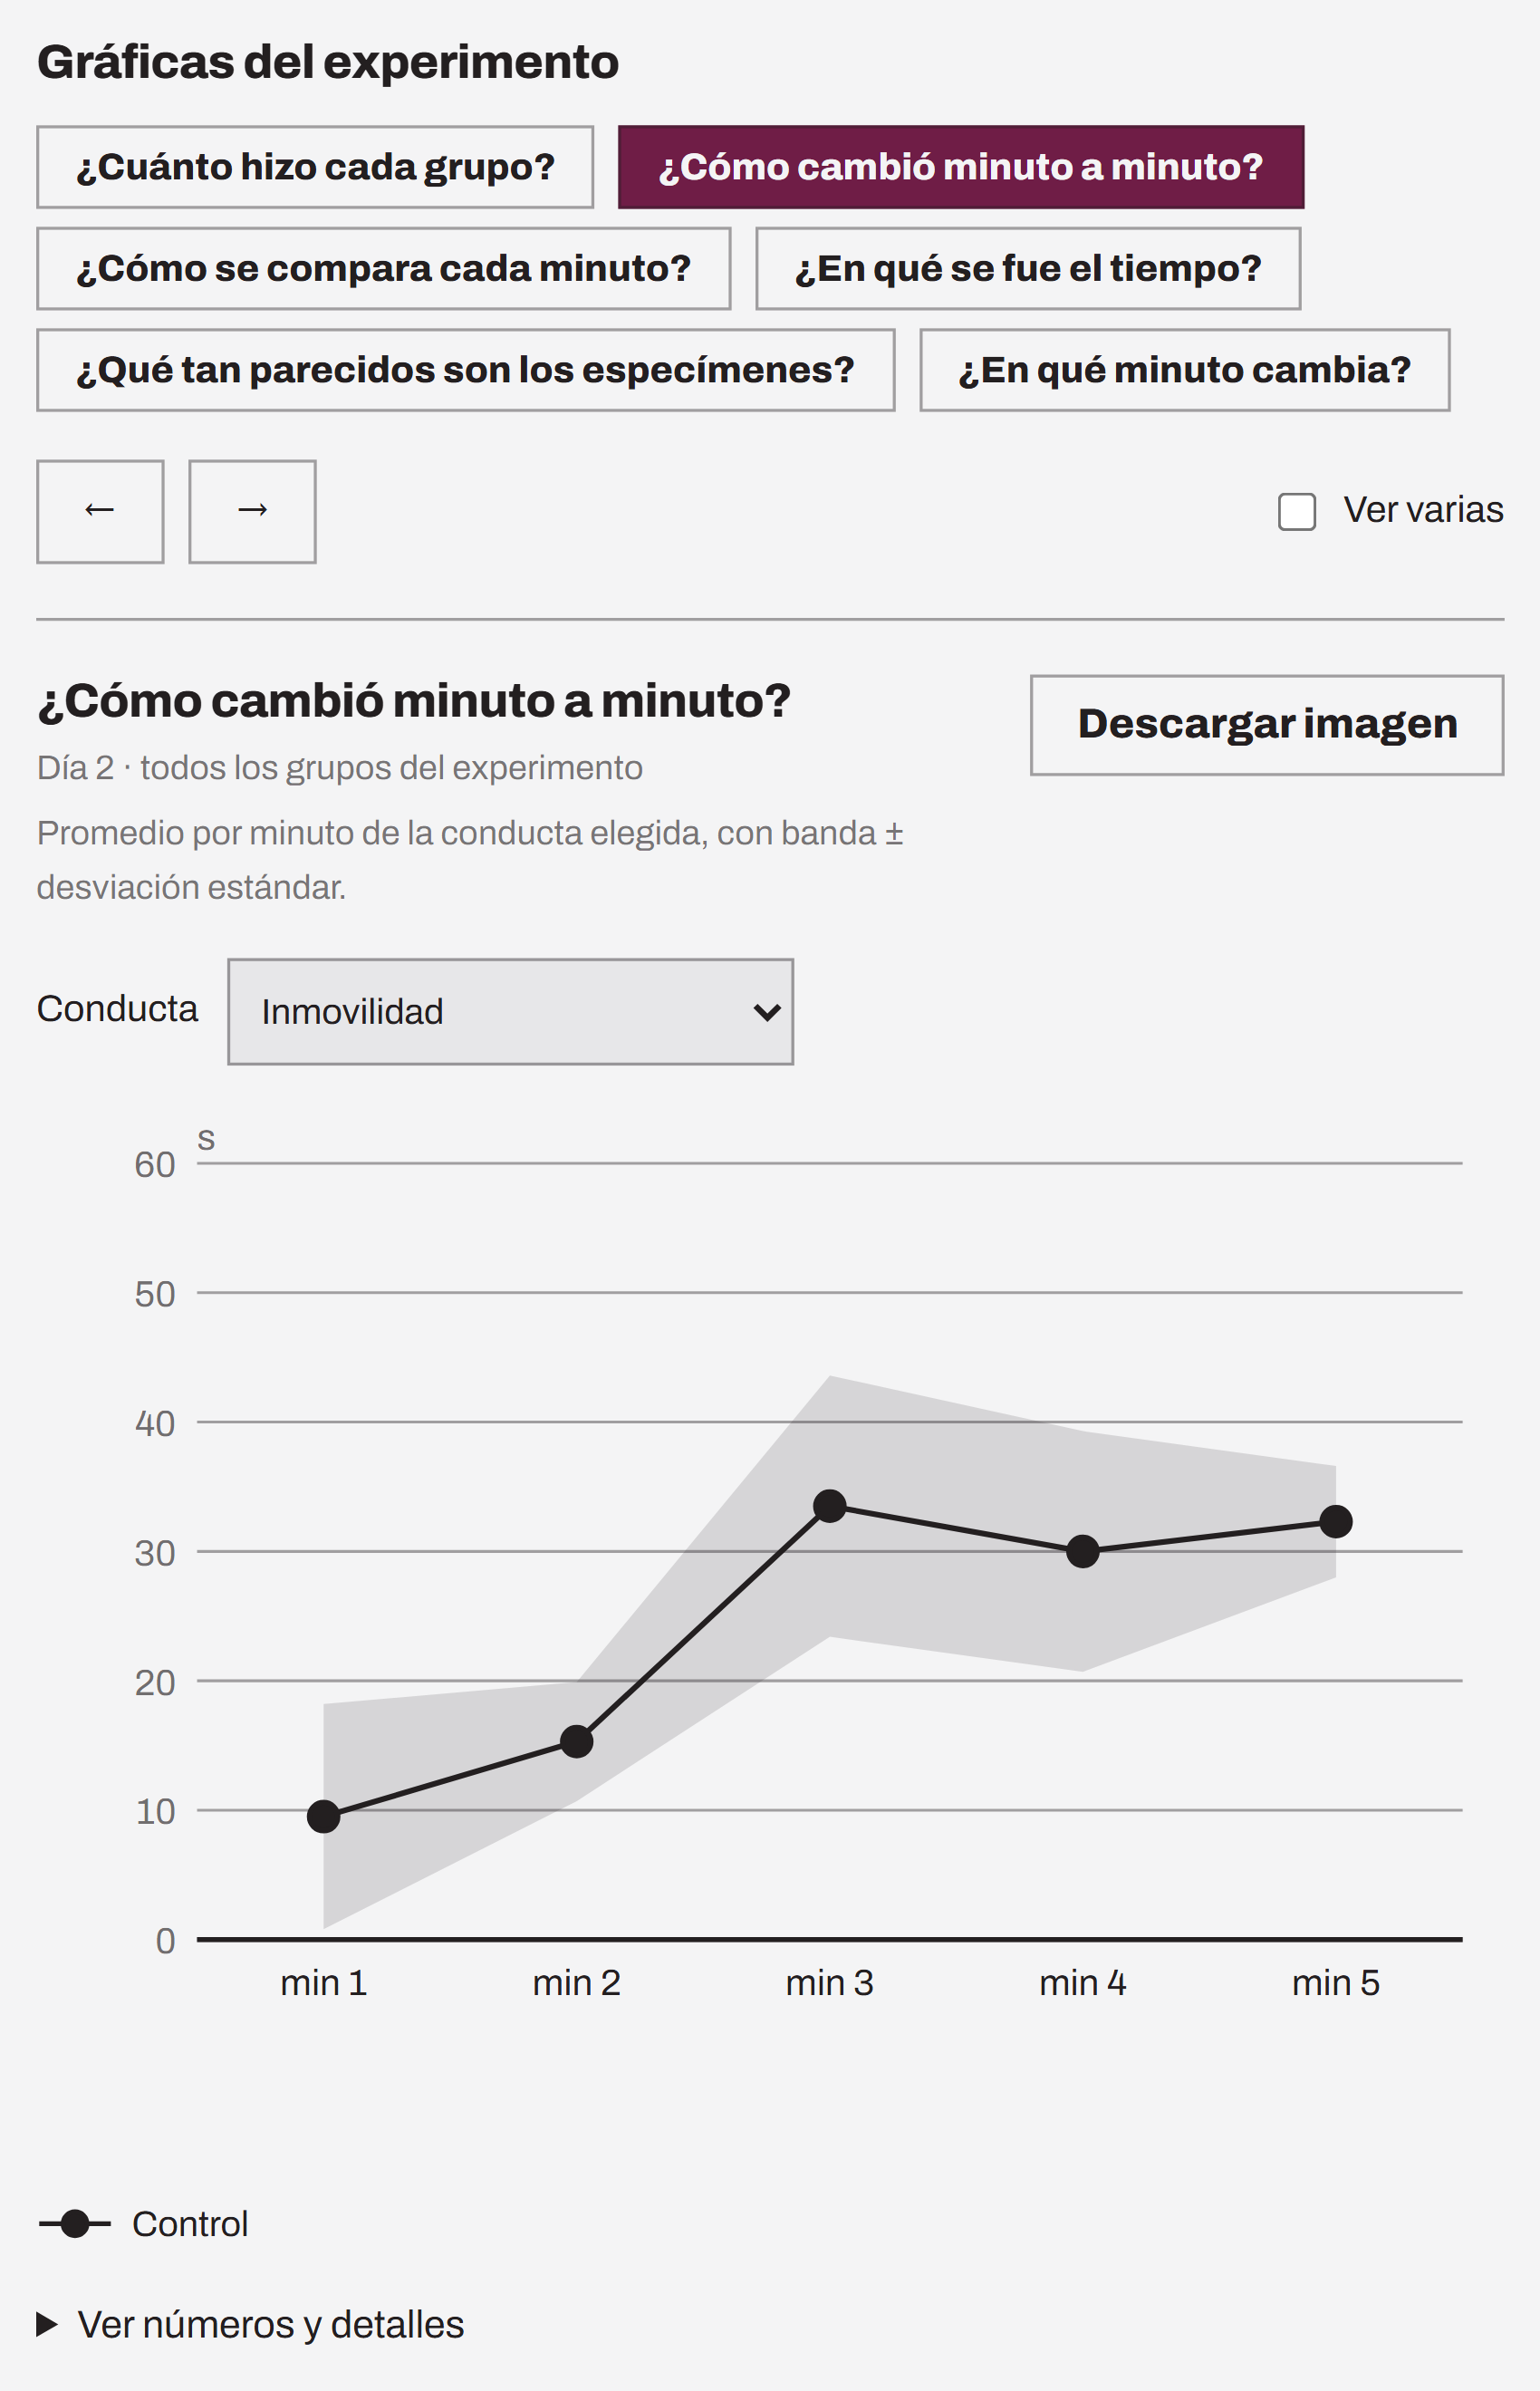
\includegraphics[width=0.7\textwidth]{figures/pruebas/33_real_grafica_curva_por_minuto}
\caption{Captura de la interfaz con el sistema completo y un video real: curva por minuto.}
\label{fig:pruebas_real_g2}
\end{figure}

\begin{figure}[tbp]
\centering
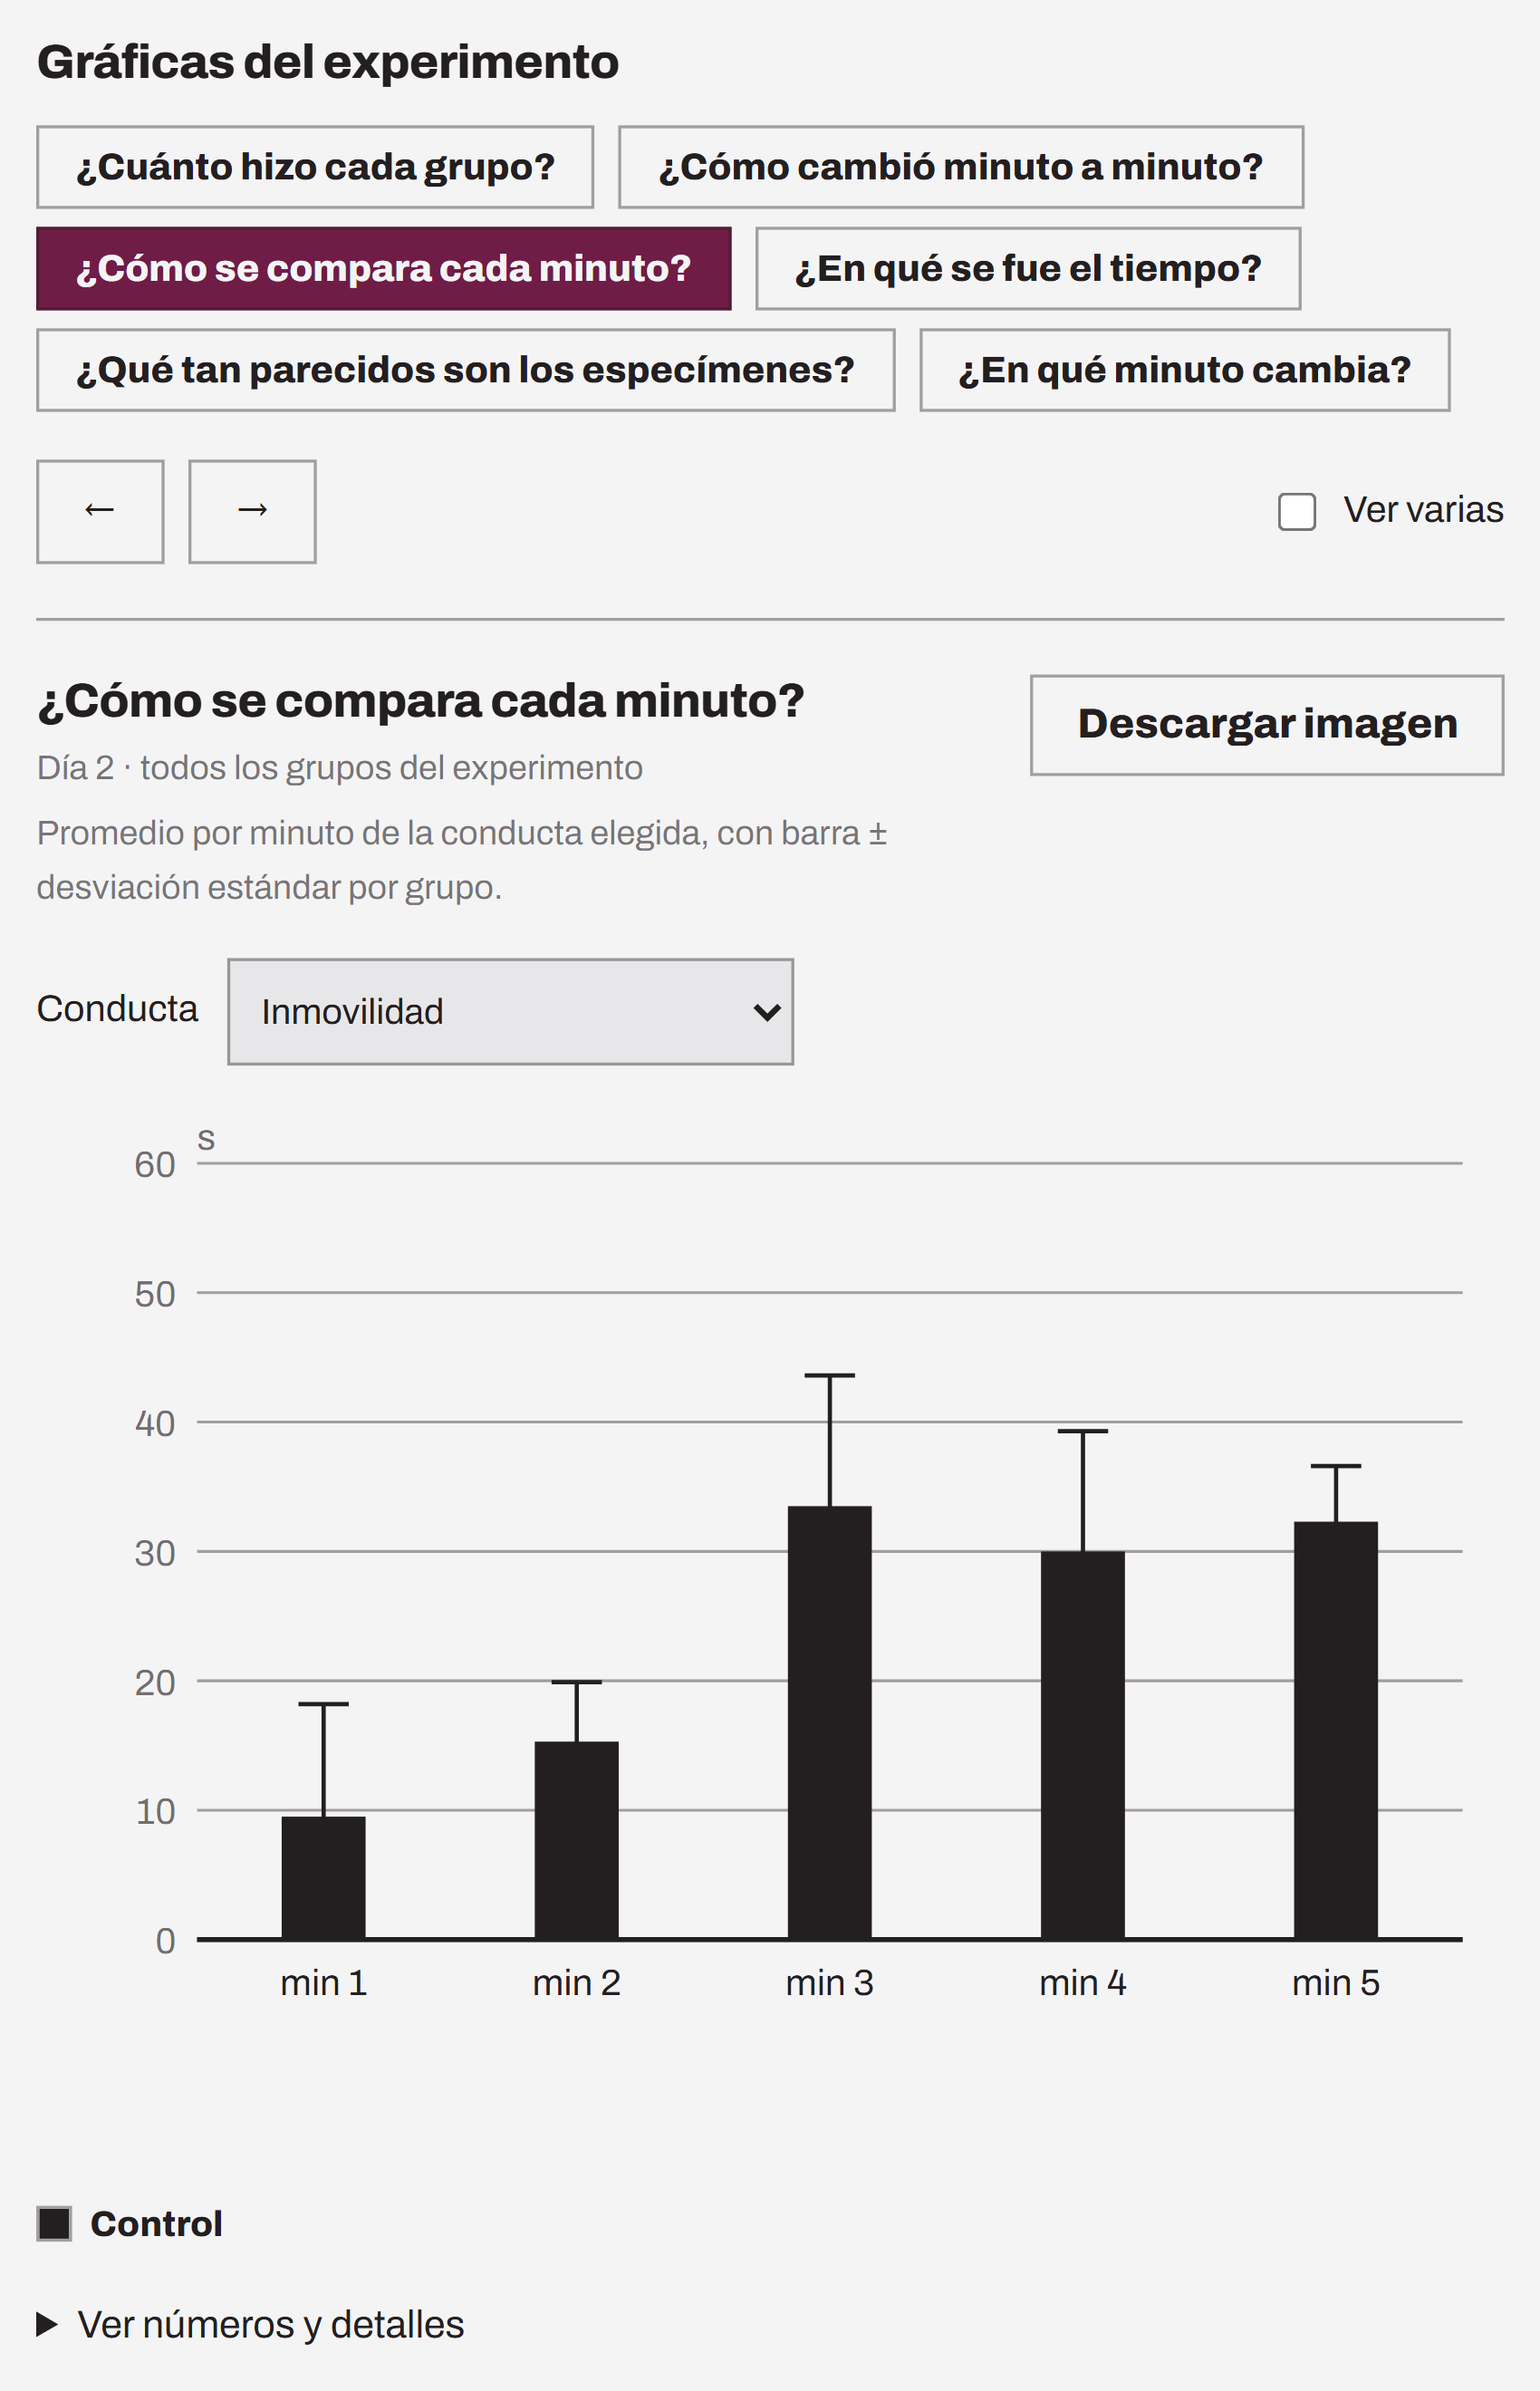
\includegraphics[width=0.7\textwidth]{figures/pruebas/34_real_grafica_barras_por_minuto}
\caption{Captura de la interfaz con el sistema completo y un video real: barras por minuto.}
\label{fig:pruebas_real_g3}
\end{figure}

\begin{figure}[tbp]
\centering
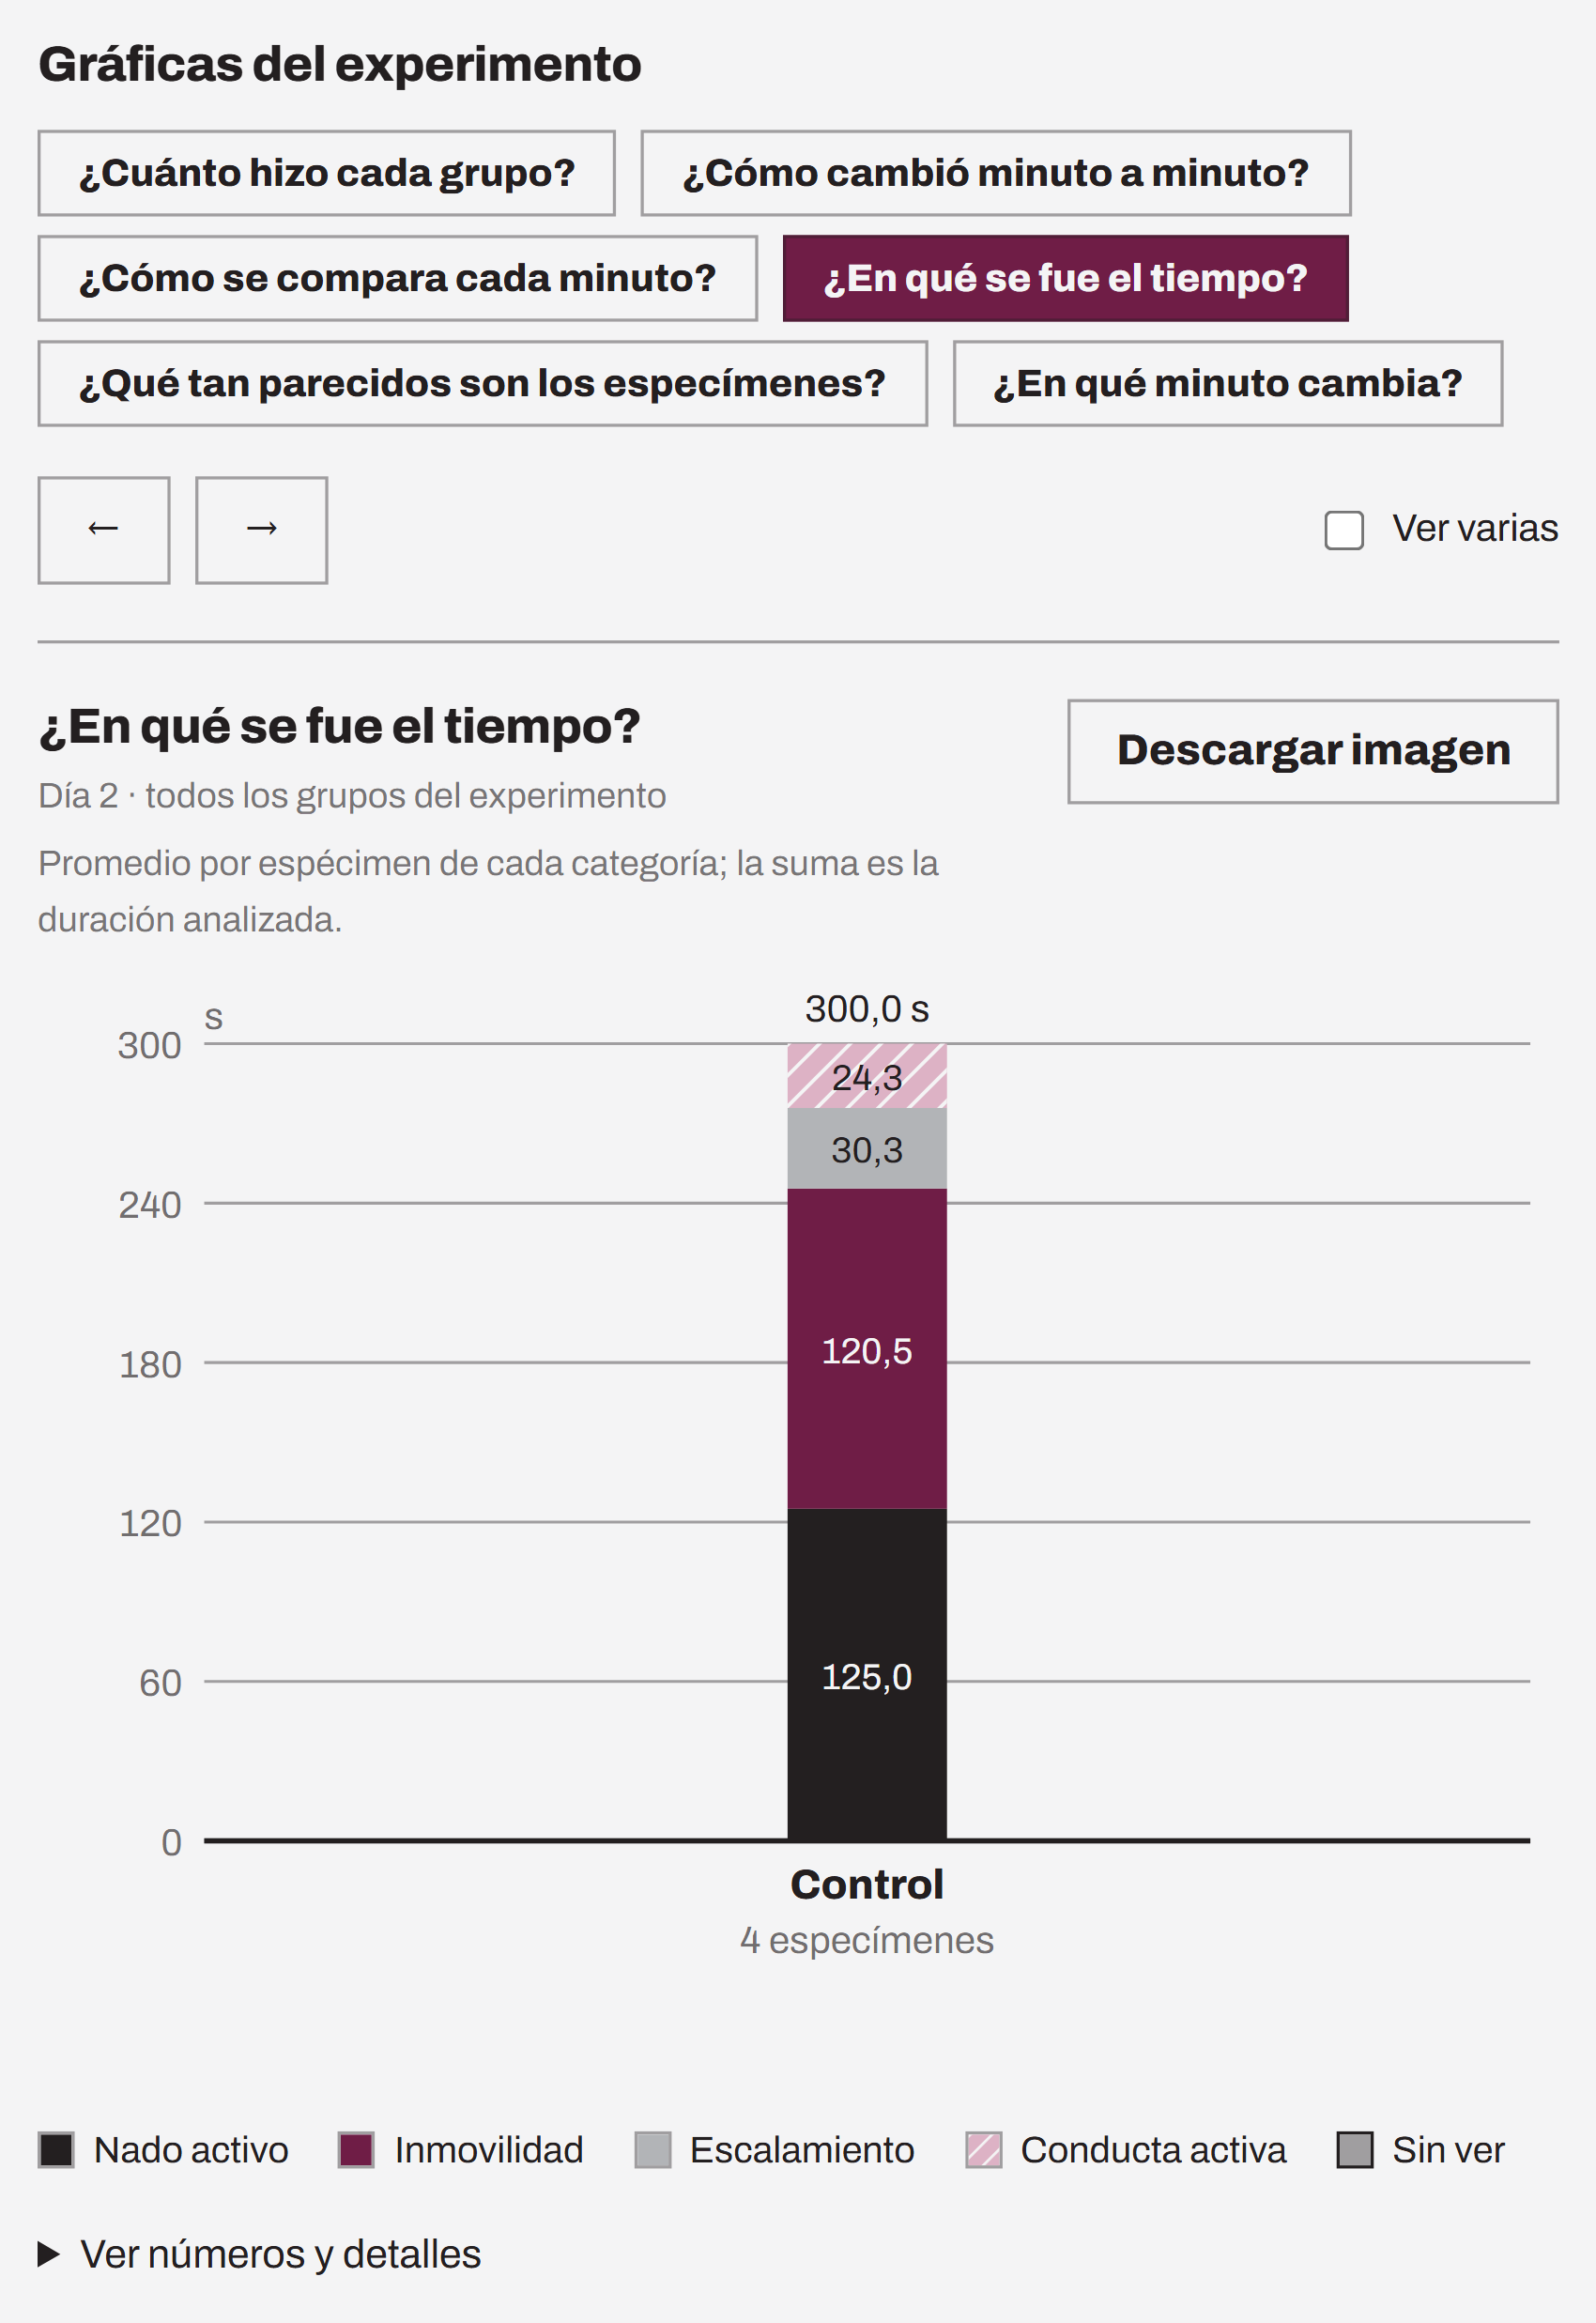
\includegraphics[width=0.7\textwidth]{figures/pruebas/35_real_grafica_reparto_de_la_duracion}
\caption{Captura de la interfaz con el sistema completo y un video real: reparto de la duración.}
\label{fig:pruebas_real_g4}
\end{figure}

\begin{figure}[tbp]
\centering
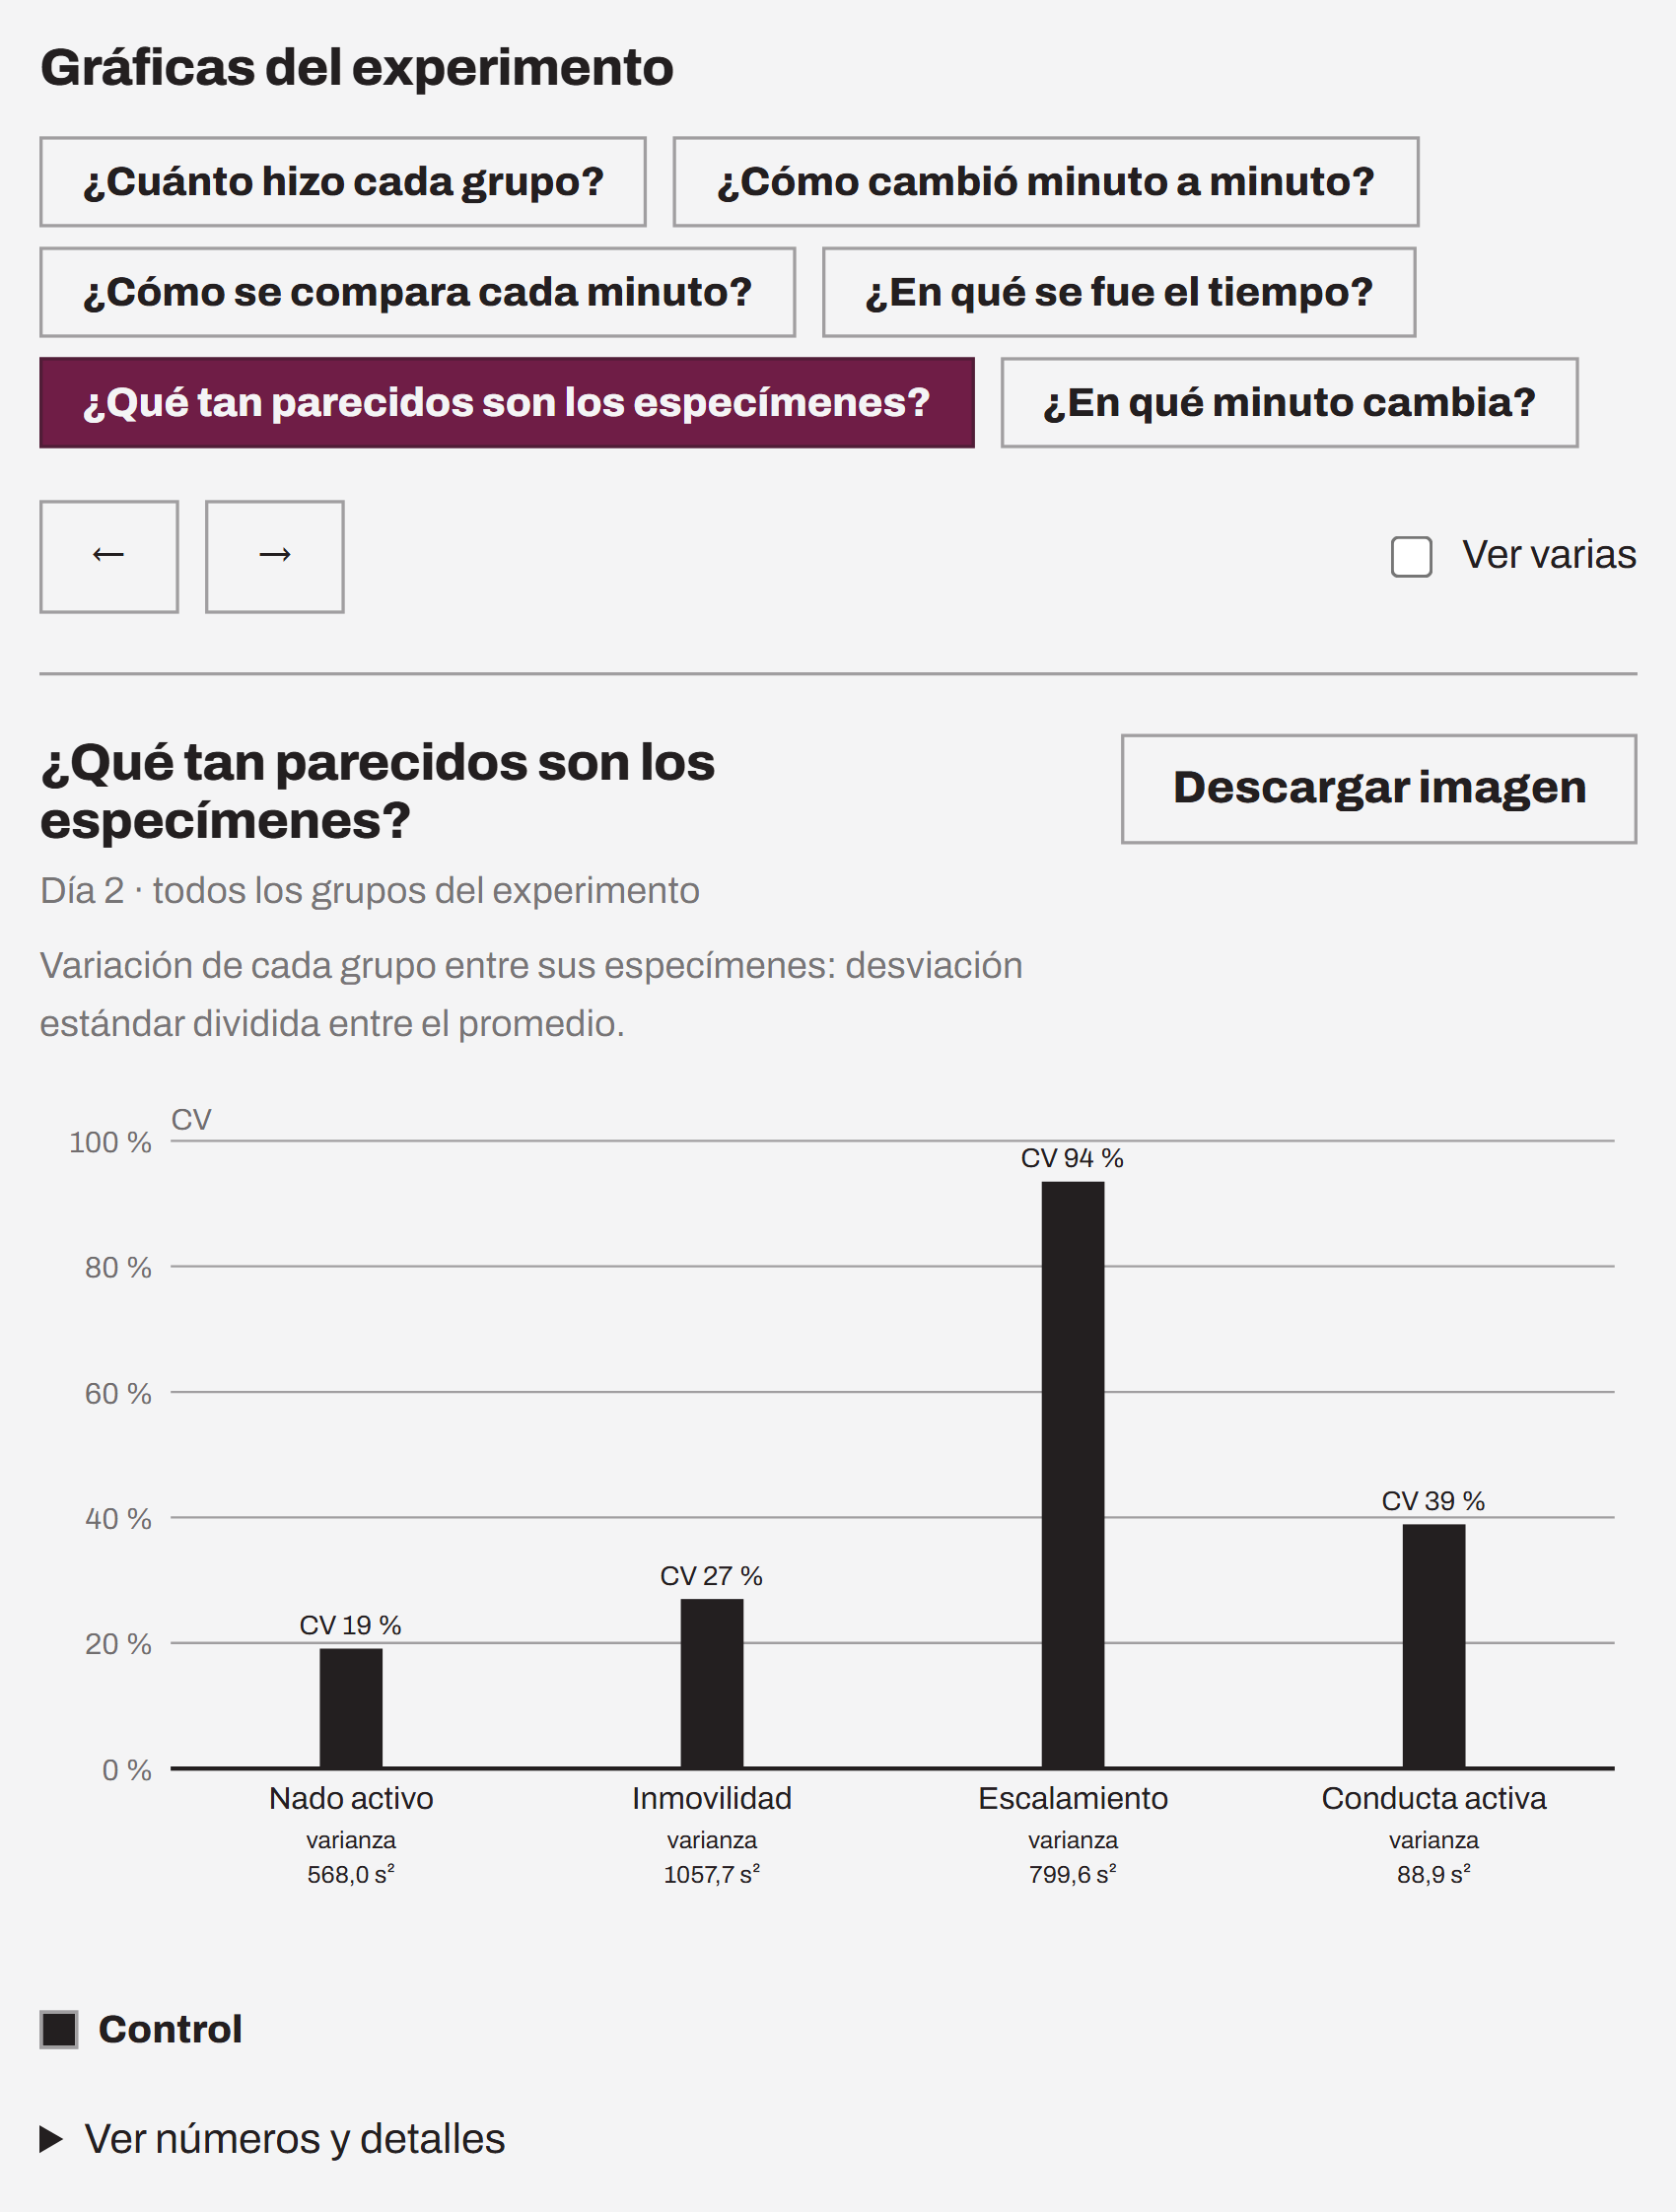
\includegraphics[width=0.8\textwidth]{figures/pruebas/36_real_grafica_variabilidad}
\caption{Captura de la interfaz con el sistema completo y un video real: variabilidad entre especímenes.}
\label{fig:pruebas_real_g5}
\end{figure}

\begin{figure}[tbp]
\centering
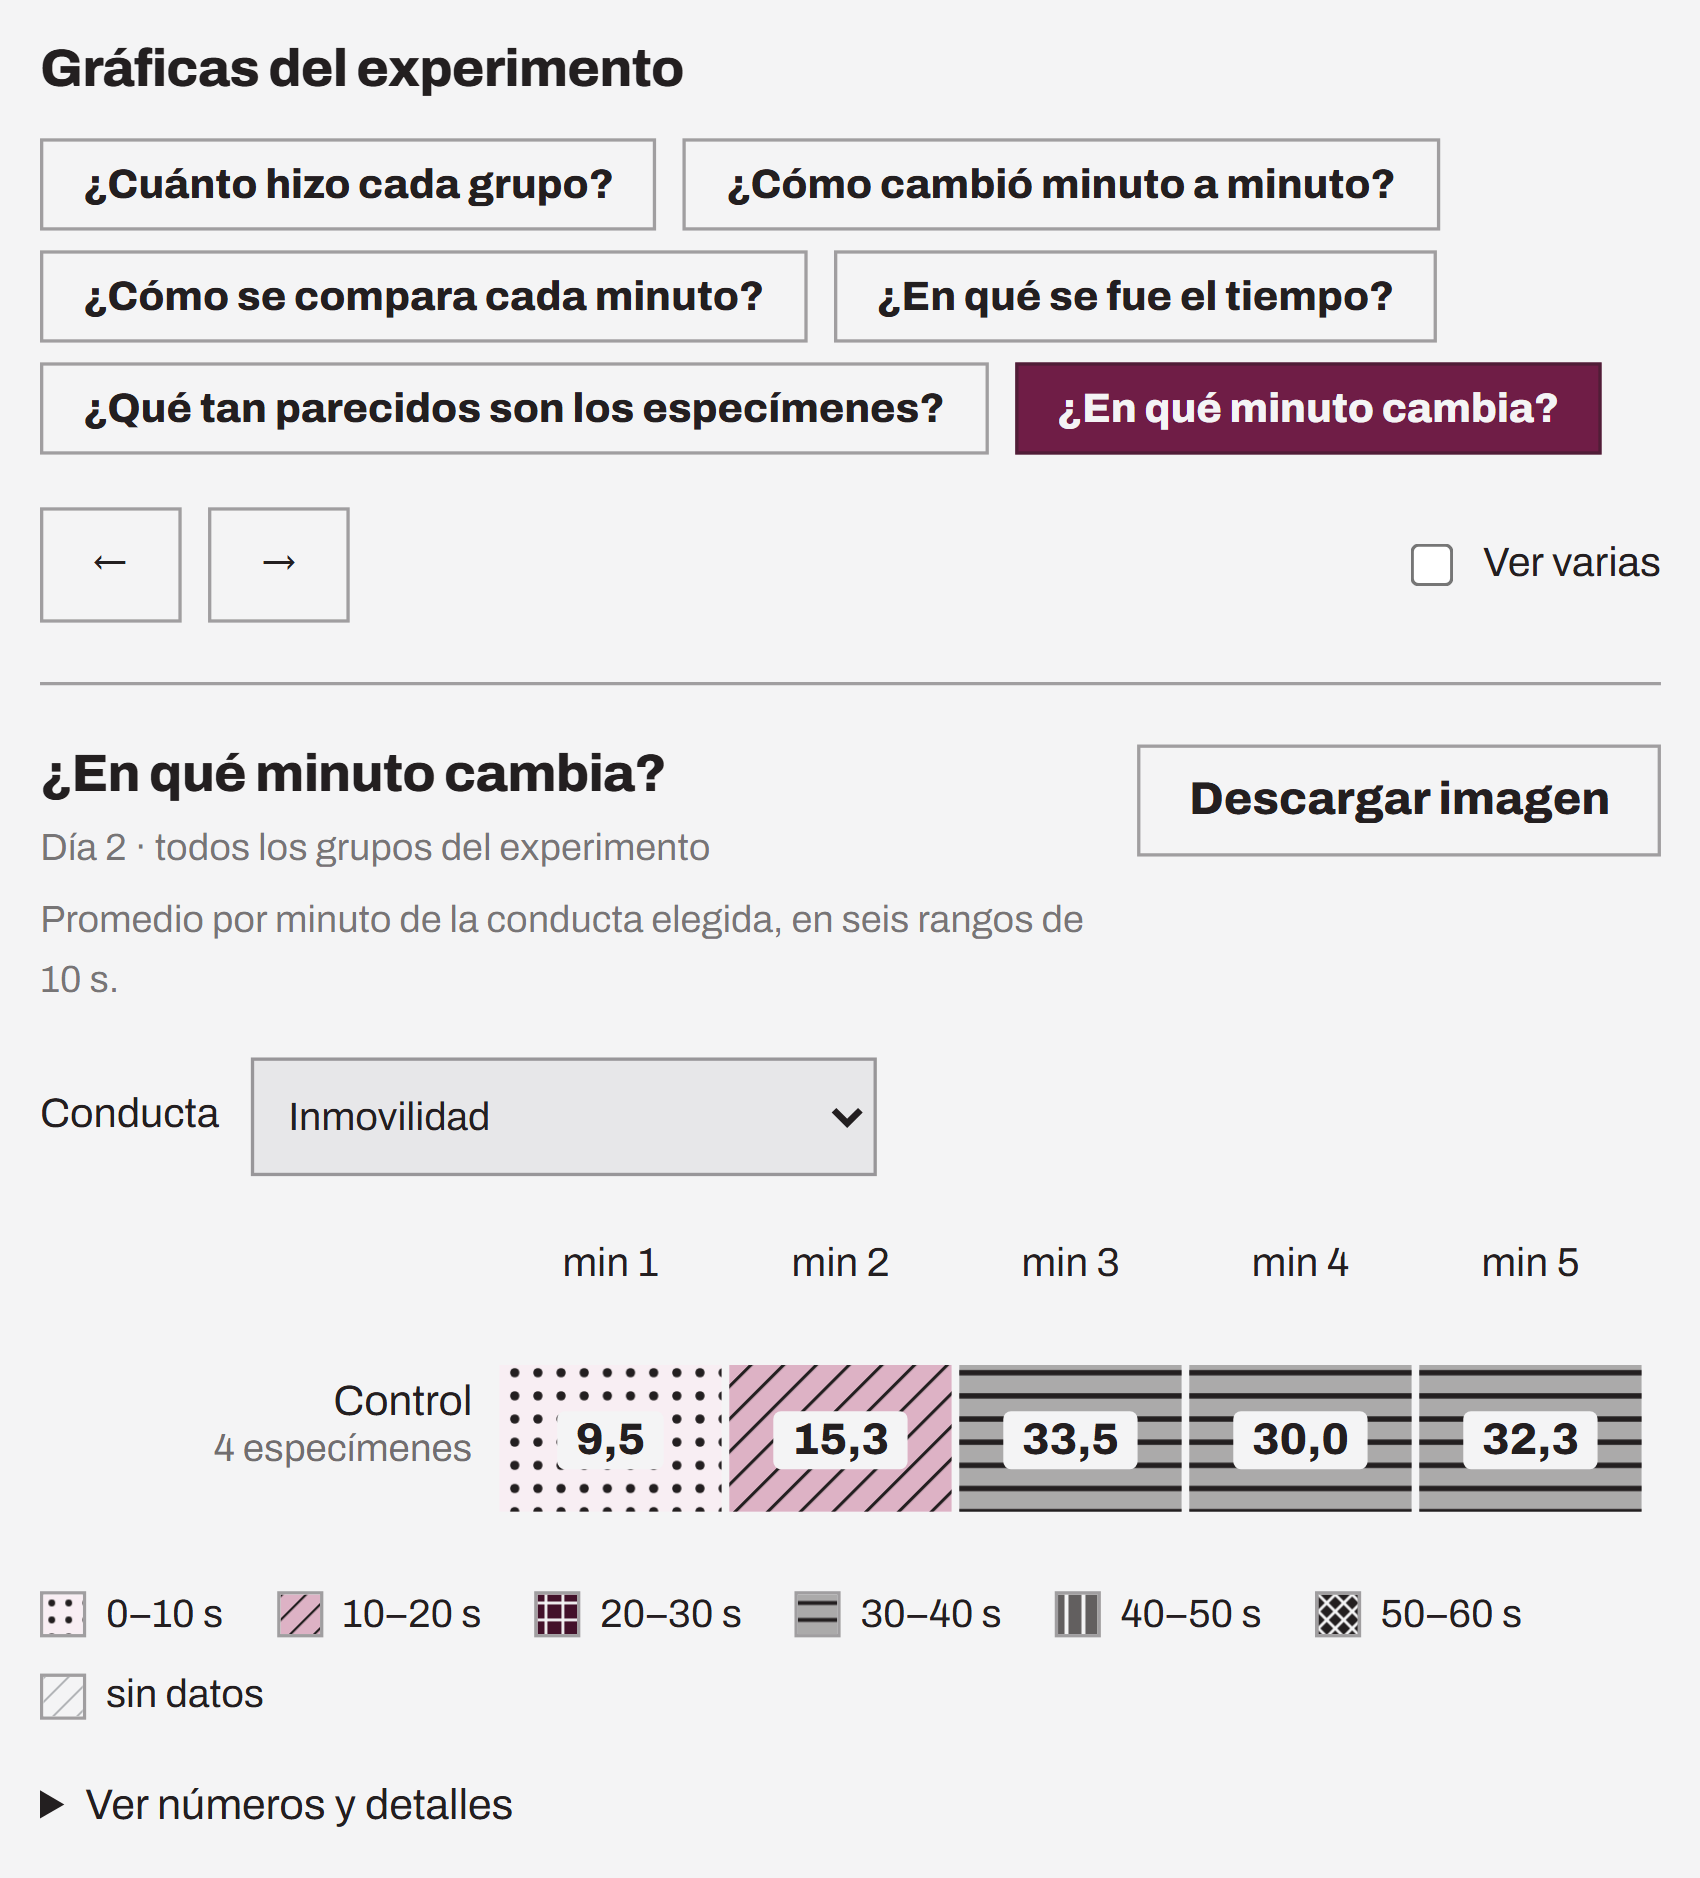
\includegraphics[width=0.7\textwidth]{figures/pruebas/37_real_grafica_mapa_por_minuto}
\caption{Captura de la interfaz con el sistema completo y un video real: mapa por minuto.}
\label{fig:pruebas_real_g6}
\end{figure}

\FloatBarrier

Las Figuras~\ref{fig:pruebas_real_esp}, \ref{fig:pruebas_real_seg} y \ref{fig:pruebas_real_min}
muestran tres de las cinco vistas del detalle por tanda: por espécimen, segundo a segundo y
minuto a minuto. La figura del segundo a segundo se recortó a las primeras filas de la tabla.

\begin{sidewaysfigure}[p]
\centering
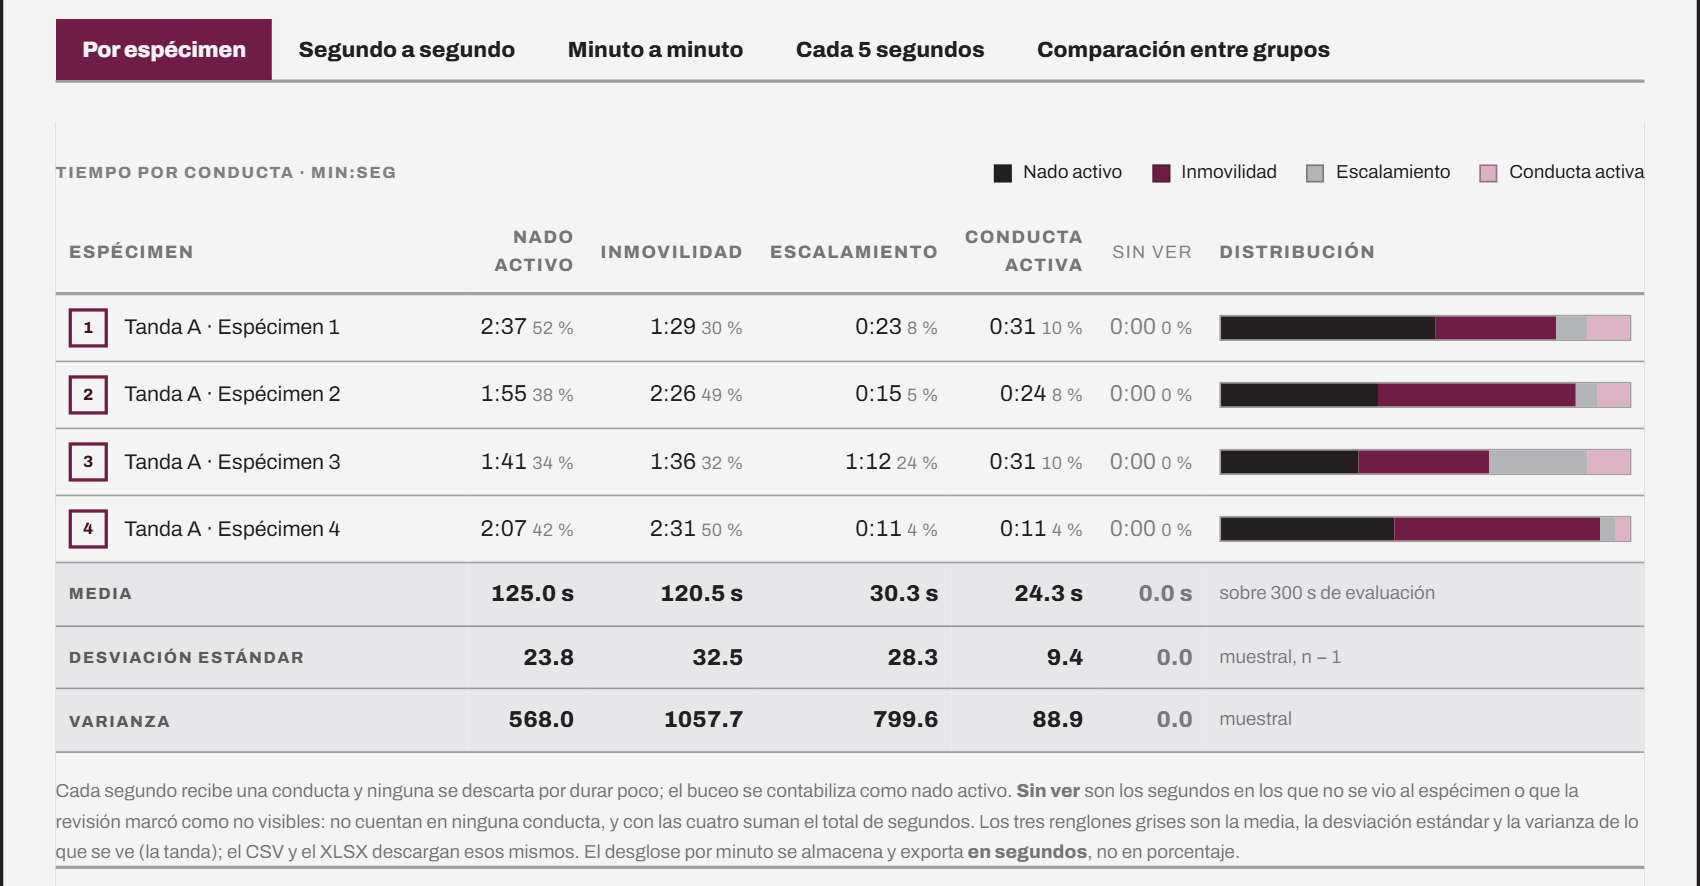
\includegraphics[width=\textheight, height=0.88\textwidth, keepaspectratio]{figures/pruebas/38_real_detalle_por_especimen}
\caption{Captura de la interfaz con el sistema completo y un video real: detalle por tanda, vista por espécimen.}
\label{fig:pruebas_real_esp}
\end{sidewaysfigure}

\begin{sidewaysfigure}[p]
\centering
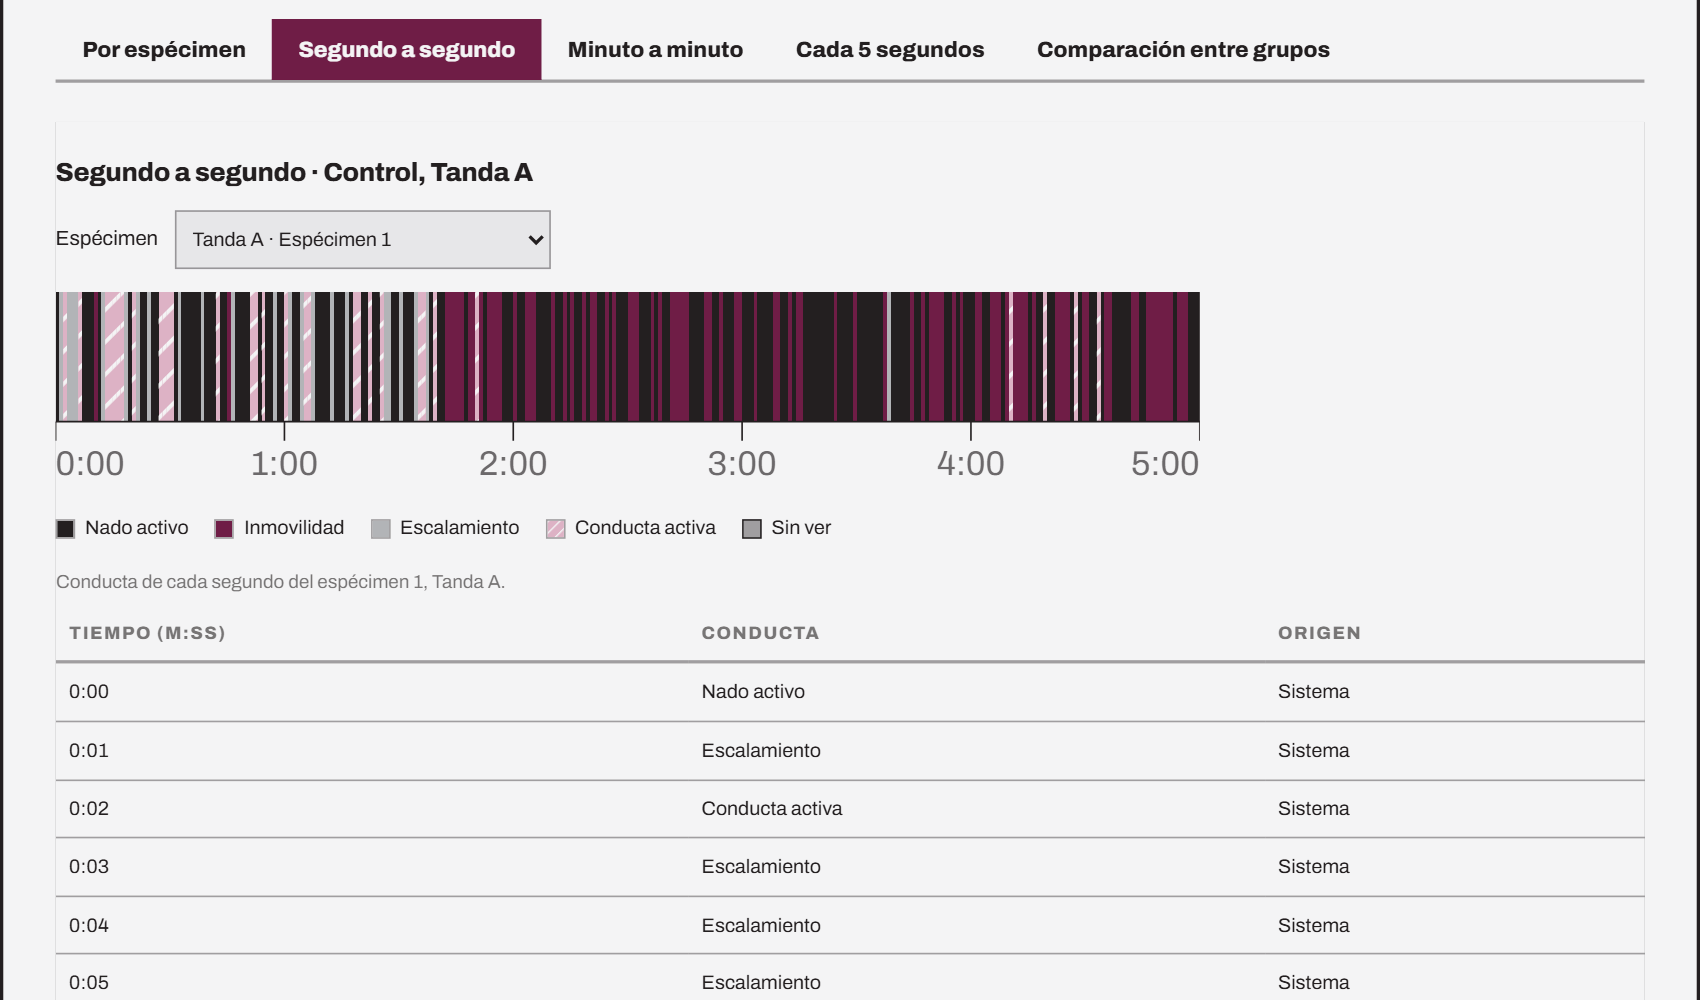
\includegraphics[width=\textheight, height=0.88\textwidth, keepaspectratio]{figures/pruebas/39_real_detalle_segundo_a_segundo_recorte}
\caption{Captura de la interfaz con el sistema completo y un video real: detalle por tanda, vista segundo a segundo, recortada a las primeras filas.}
\label{fig:pruebas_real_seg}
\end{sidewaysfigure}

\begin{sidewaysfigure}[p]
\centering
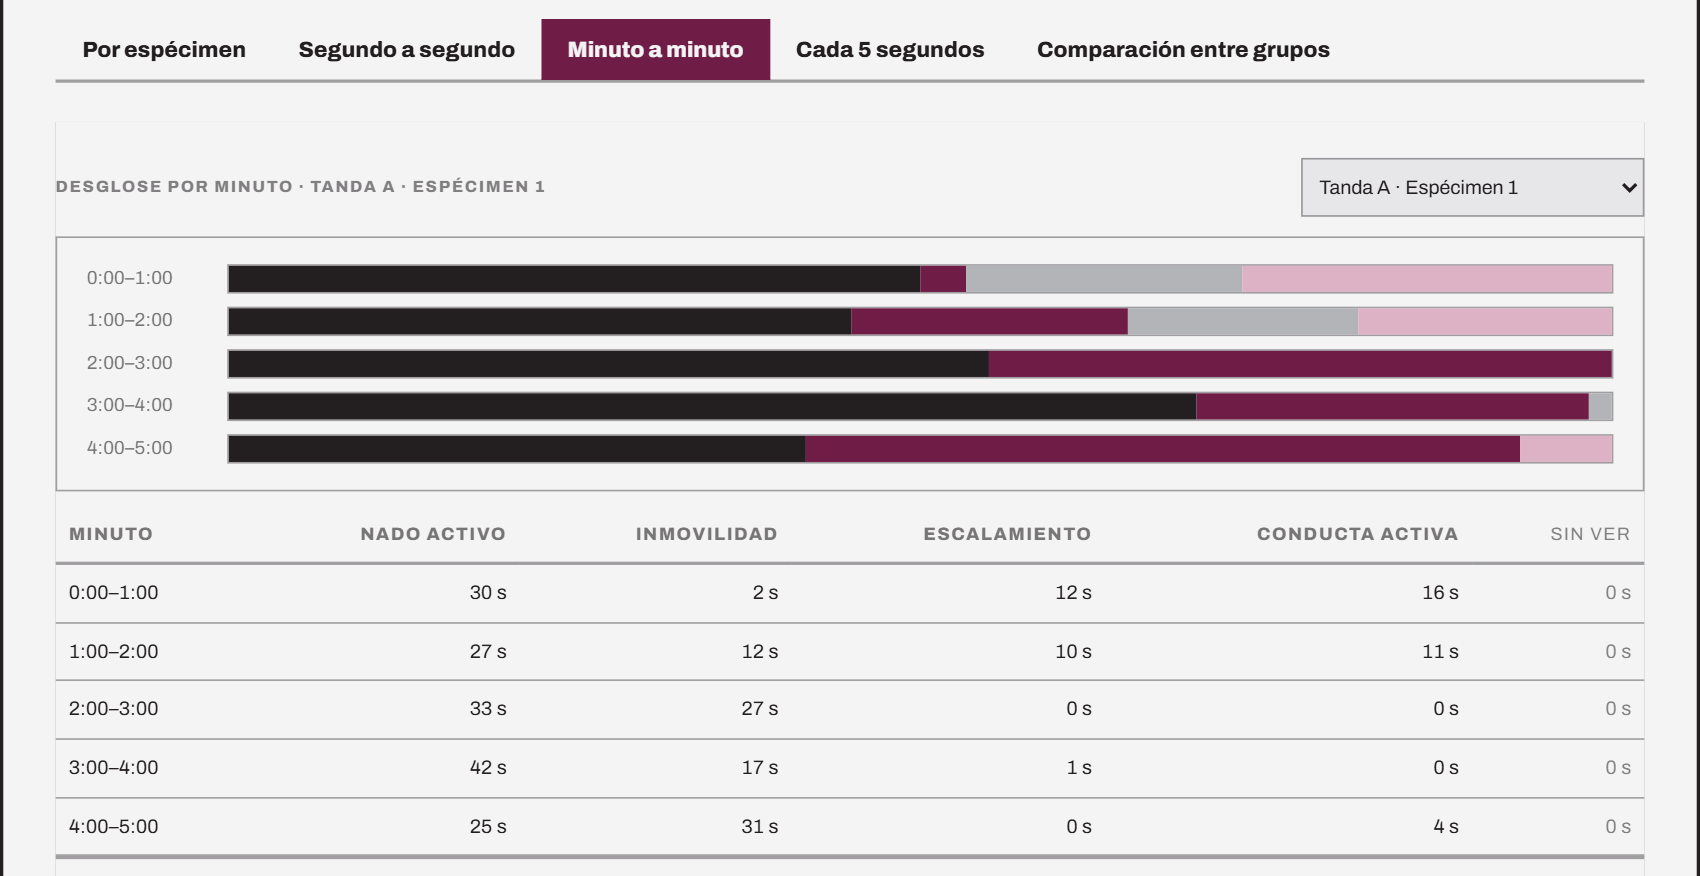
\includegraphics[width=\textheight, height=0.88\textwidth, keepaspectratio]{figures/pruebas/40_real_detalle_minuto_a_minuto}
\caption{Captura de la interfaz con el sistema completo y un video real: detalle por tanda, vista minuto a minuto.}
\label{fig:pruebas_real_min}
\end{sidewaysfigure}

\FloatBarrier

\subsection{Revisión segundo a segundo}

La Figura~\ref{fig:pruebas_real_rev_a} y su continuación (Figura~\ref{fig:pruebas_real_rev_b})
muestran la revisión segundo a segundo con el video real, los recuadros de los cuatro cilindros
y las líneas de conducta de cada espécimen.

\begin{figure}[tbp]
\centering
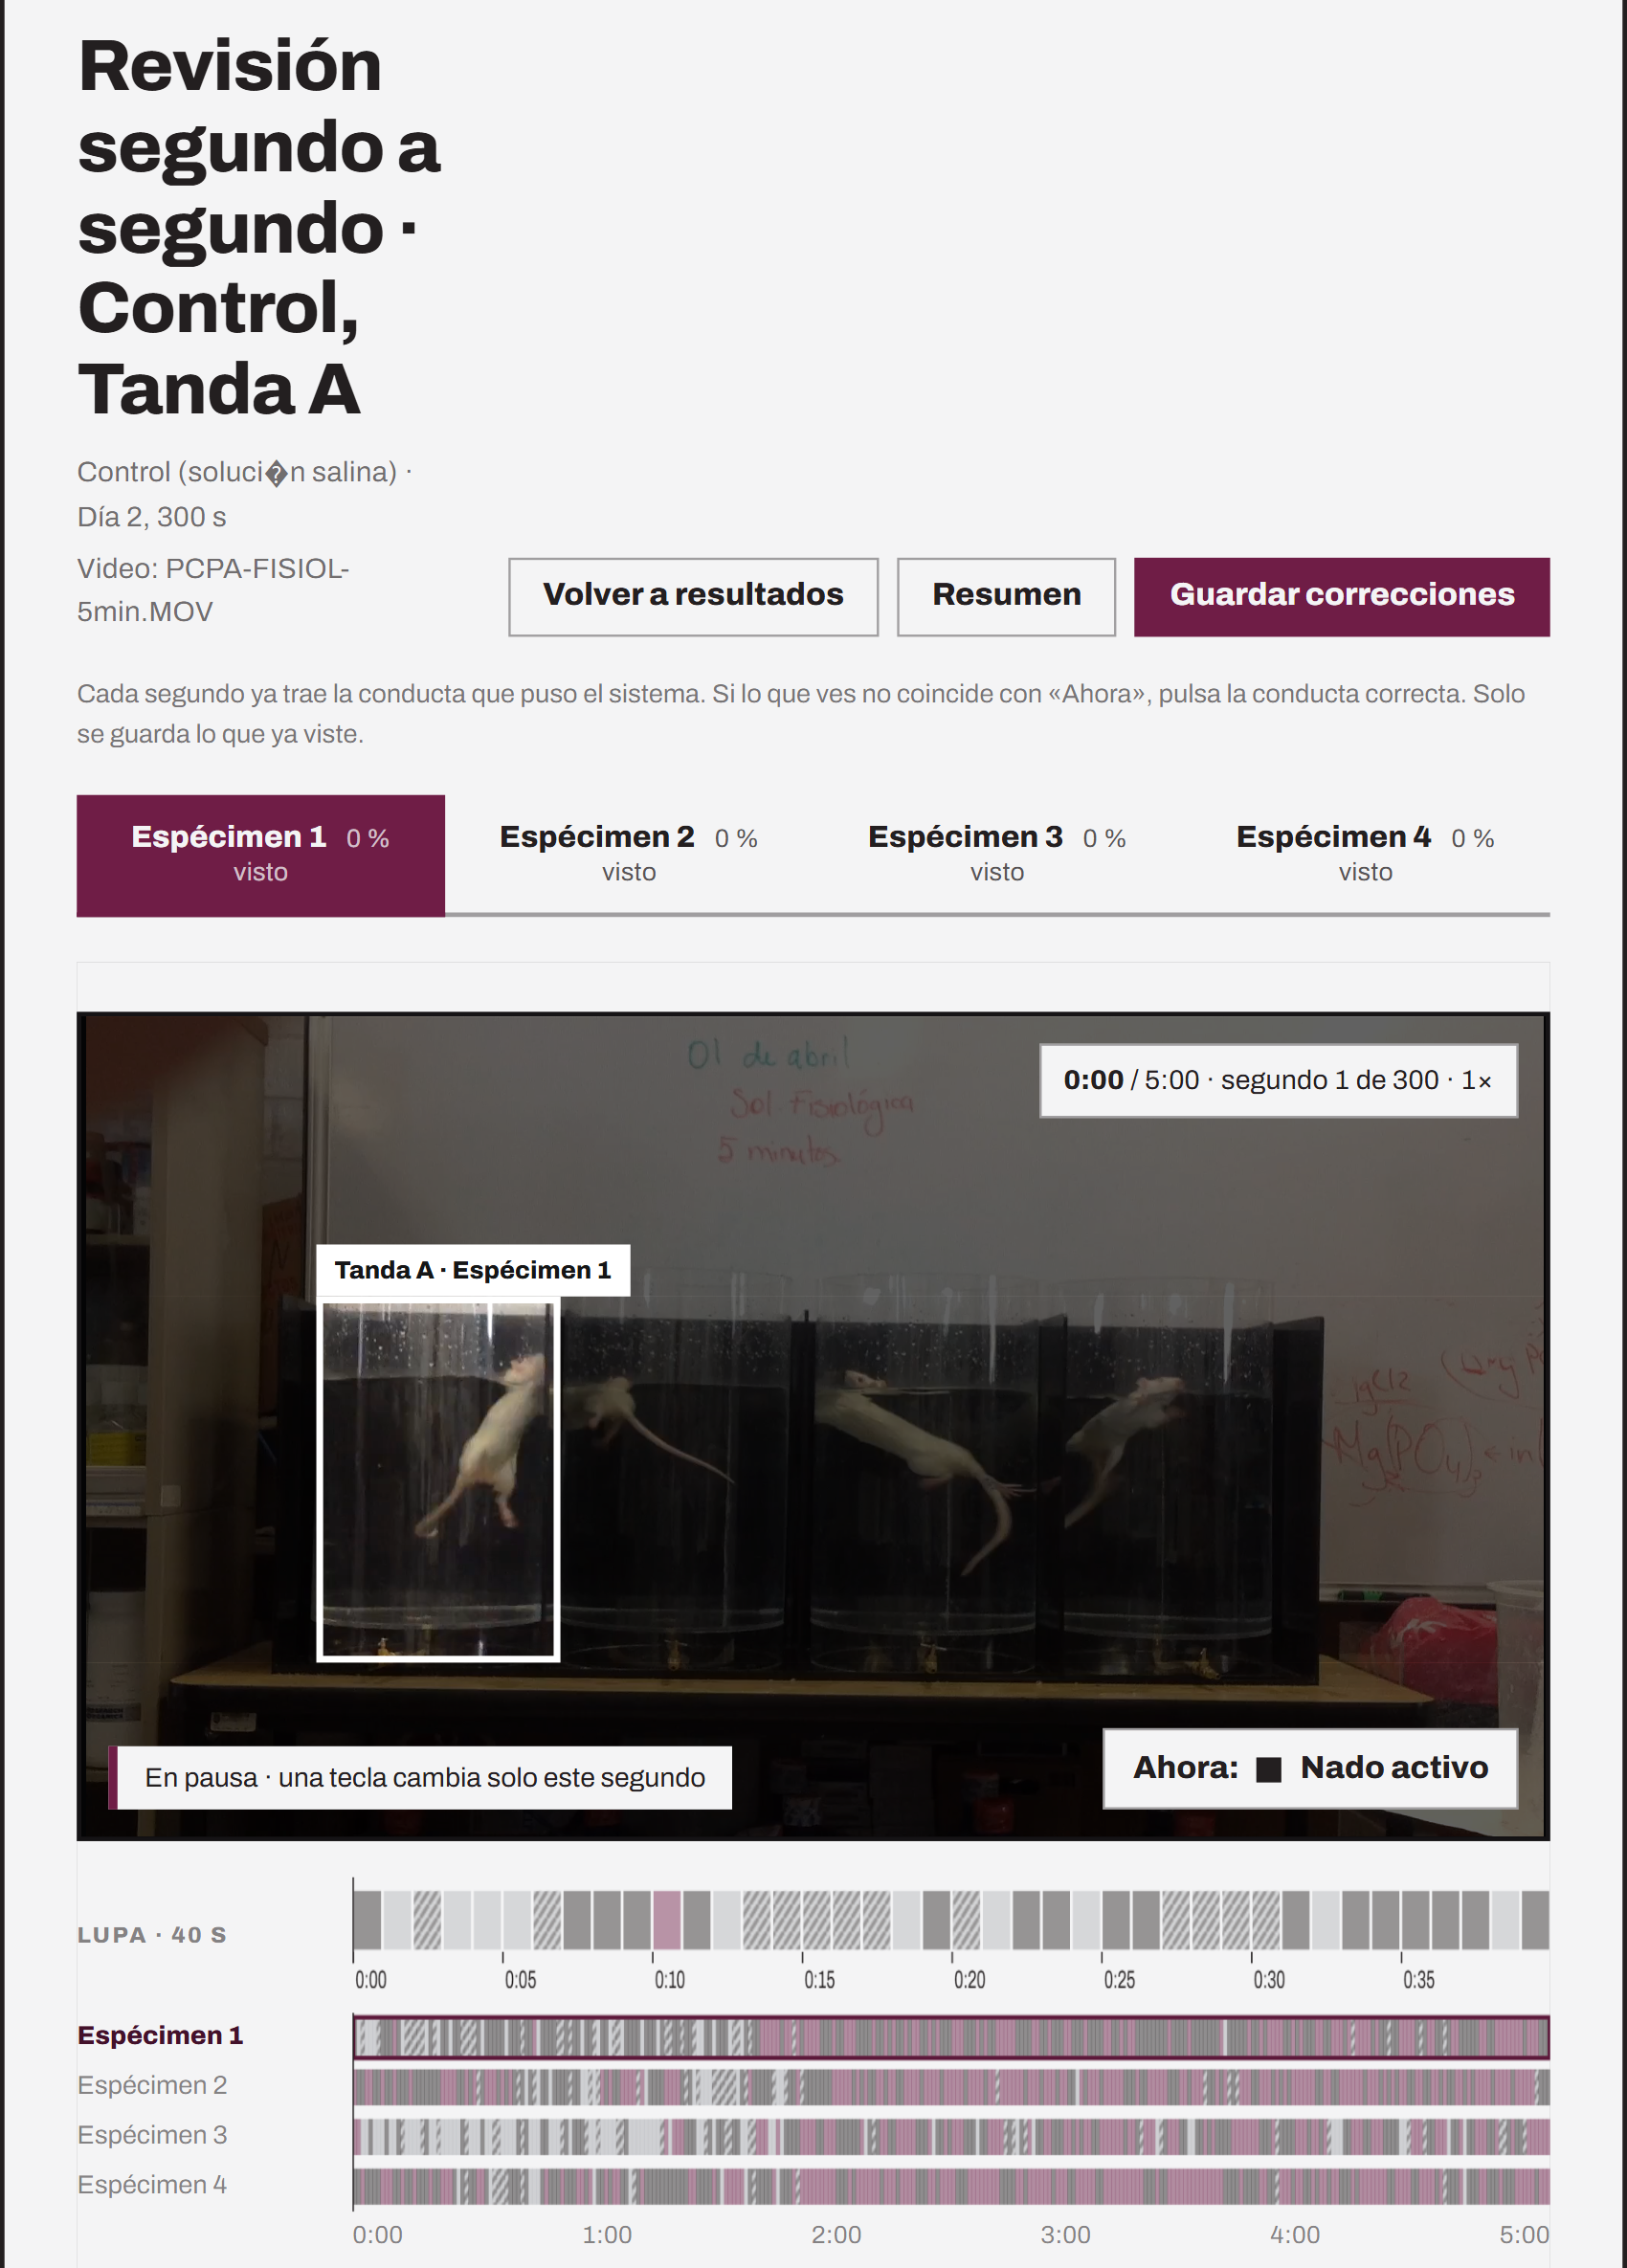
\includegraphics[width=0.95\textwidth]{figures/pruebas/43_real_revision_segundo_a_segundo_a}
\caption{Captura de la interfaz con el sistema completo y un video real: revisión segundo a segundo, con el video, los recuadros de los cilindros y las líneas de conducta.}
\label{fig:pruebas_real_rev_a}
\end{figure}

\begin{figure}[tbp]
\ContinuedFloat
\centering
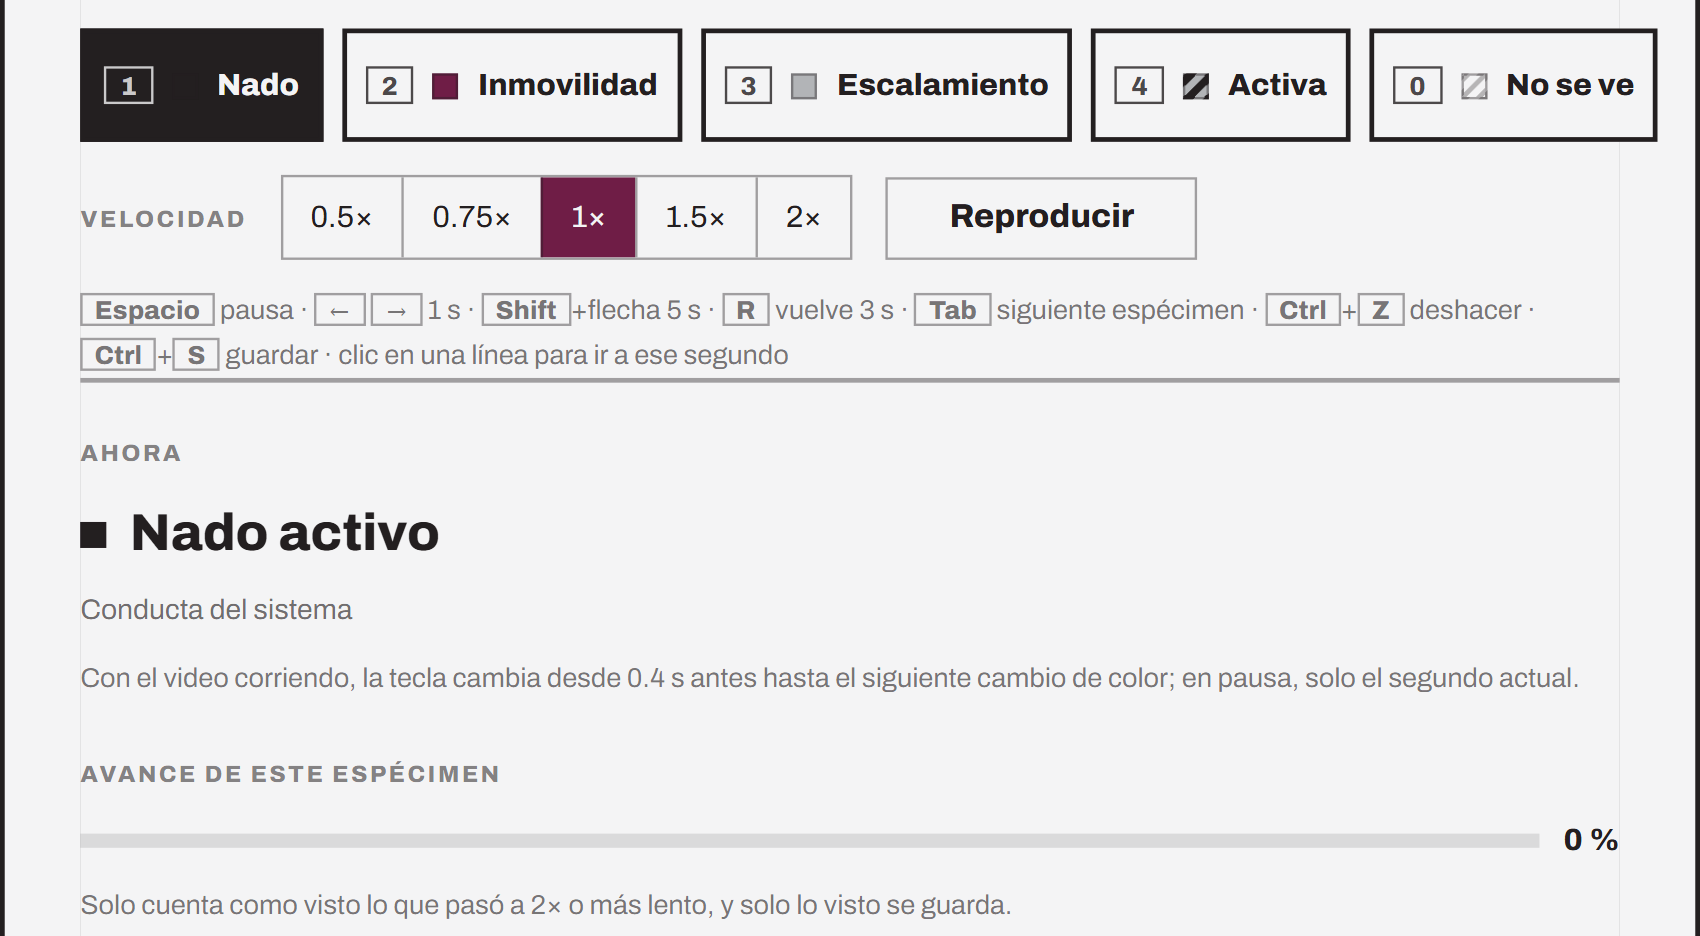
\includegraphics[width=0.95\textwidth]{figures/pruebas/43_real_revision_segundo_a_segundo_b}
\caption[]{Captura de la interfaz con el sistema completo y un video real: revisión segundo a segundo, con las conductas, la velocidad y el avance del espécimen (continuación).}
\label{fig:pruebas_real_rev_b}
\end{figure}

\FloatBarrier

\subsection{Cuentas}

Las Figuras~\ref{fig:pruebas_real_cuentas} y \ref{fig:pruebas_real_alta} muestran la
administración de cuentas y el alta de una cuenta por el Administrador. Las cuentas que aparecen
son cuentas de prueba.

\begin{figure}[tbp]
\centering
\makebox[\textwidth][c]{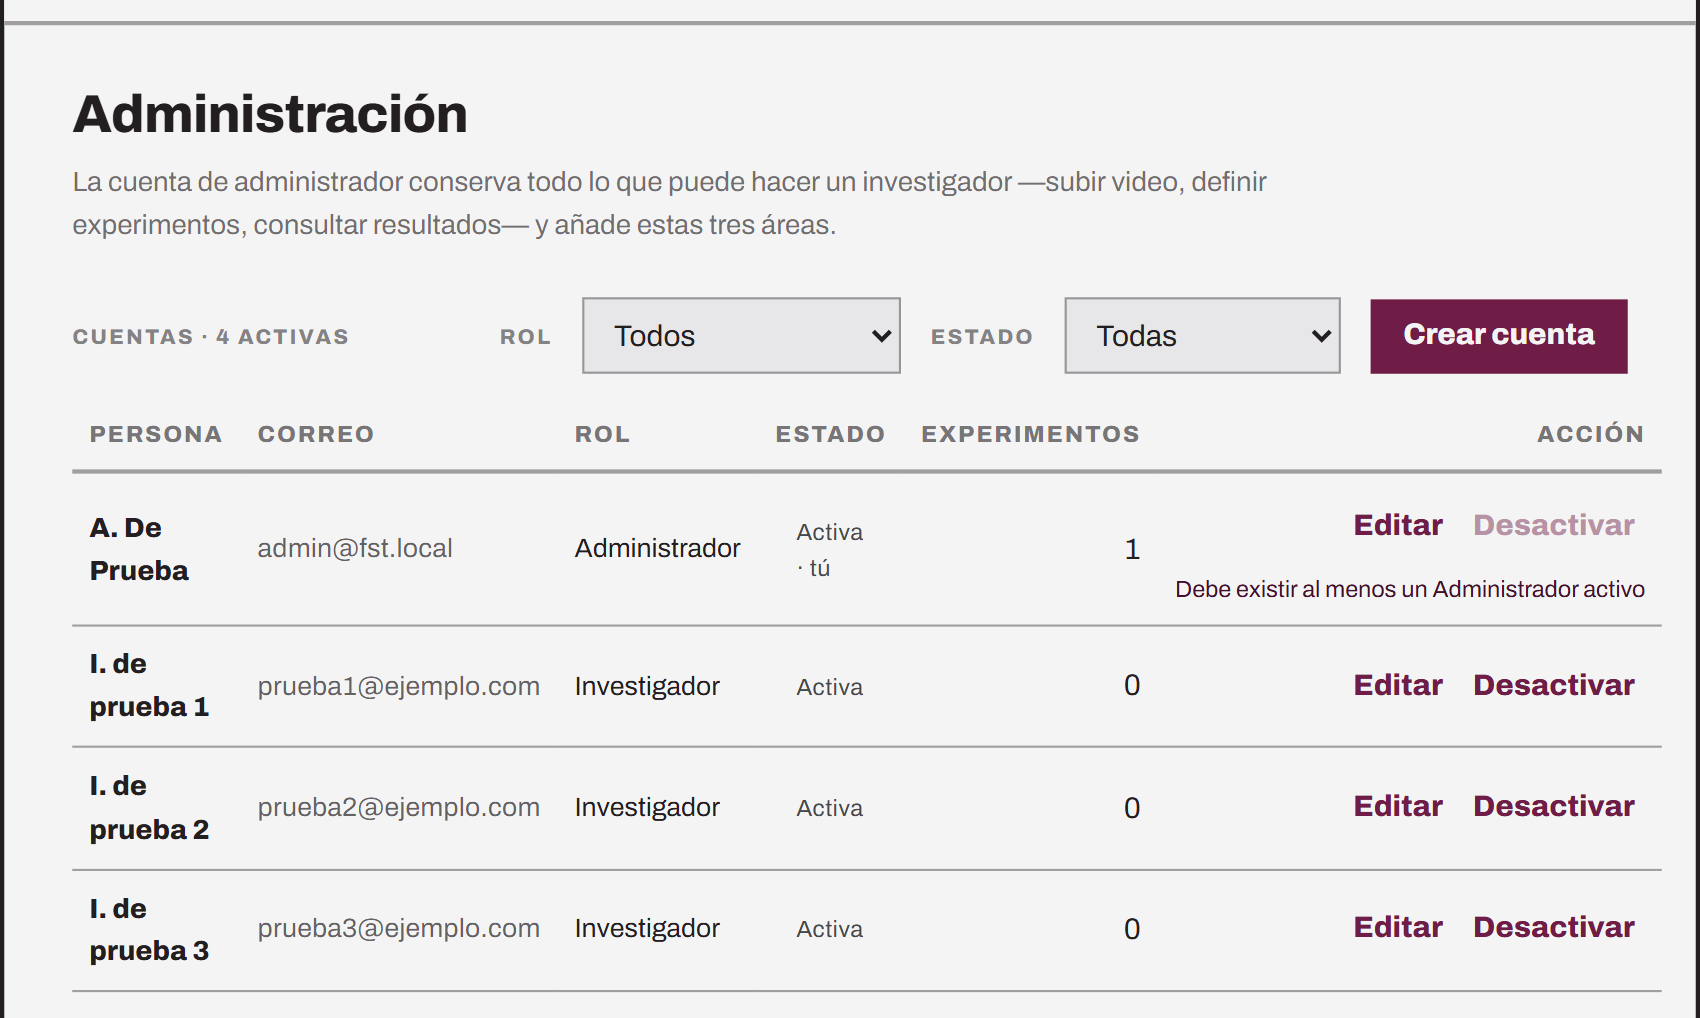
\includegraphics[width=17cm]{figures/pruebas/46_real_administracion_de_cuentas}}
\caption{Captura de la interfaz con el sistema completo: administración de cuentas, con los filtros de rol y de estado. Todas las cuentas son de prueba.}
\label{fig:pruebas_real_cuentas}
\end{figure}

\begin{figure}[tbp]
\centering
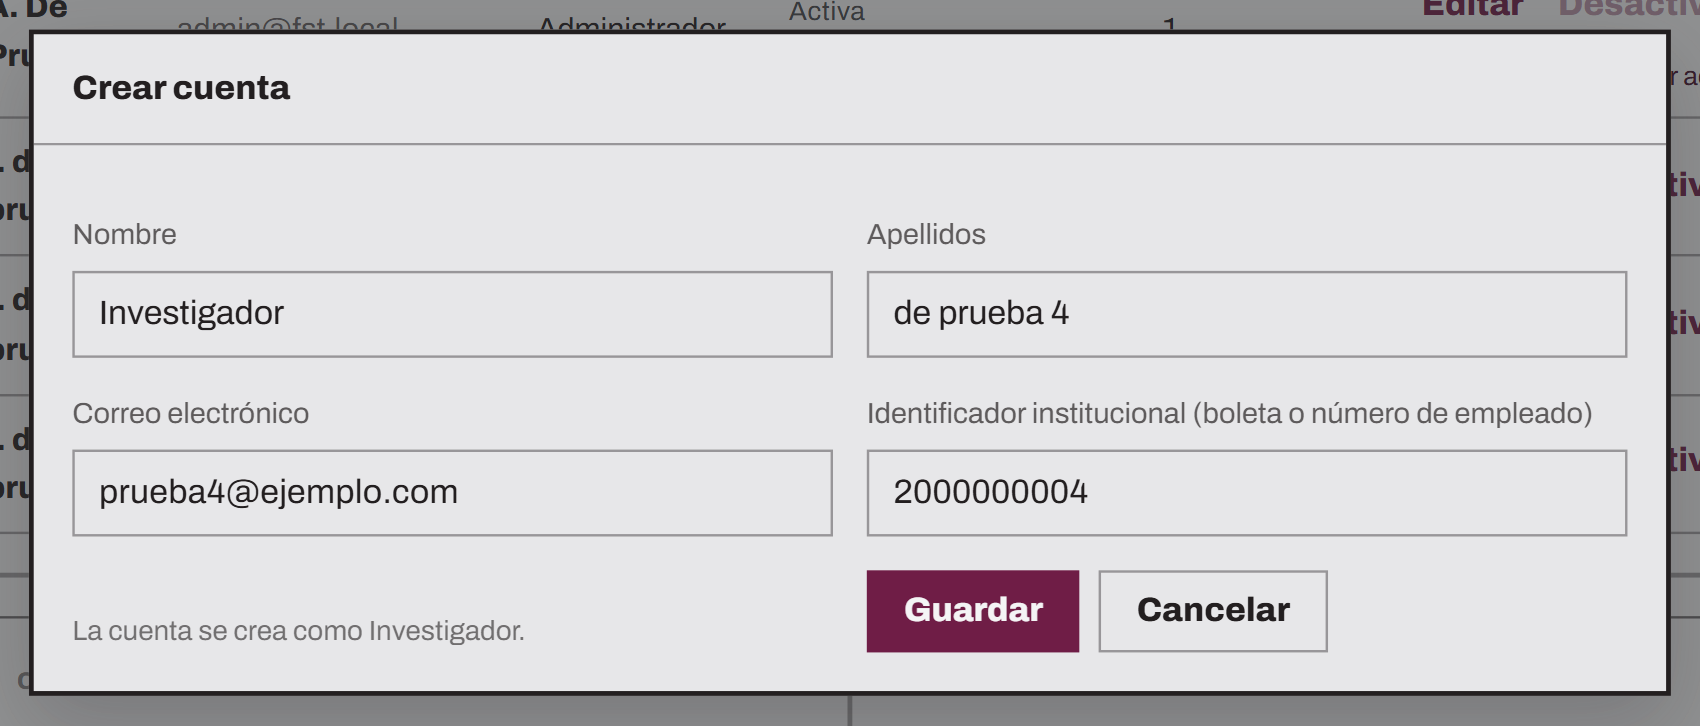
\includegraphics[width=0.95\textwidth]{figures/pruebas/47_real_alta_de_cuenta}
\caption{Captura de la interfaz con el sistema completo: alta de una cuenta por el Administrador, con datos de prueba.}
\label{fig:pruebas_real_alta}
\end{figure}

\FloatBarrier

\subsection{Experimentos}

La Figura~\ref{fig:pruebas_real_crear} muestra el formulario para crear un experimento, y la
Figura~\ref{fig:pruebas_real_lista} la lista de experimentos con el filtro de estado
«Completado», donde aparece el experimento de esta verificación.

\begin{figure}[tbp]
\centering
\makebox[\textwidth][c]{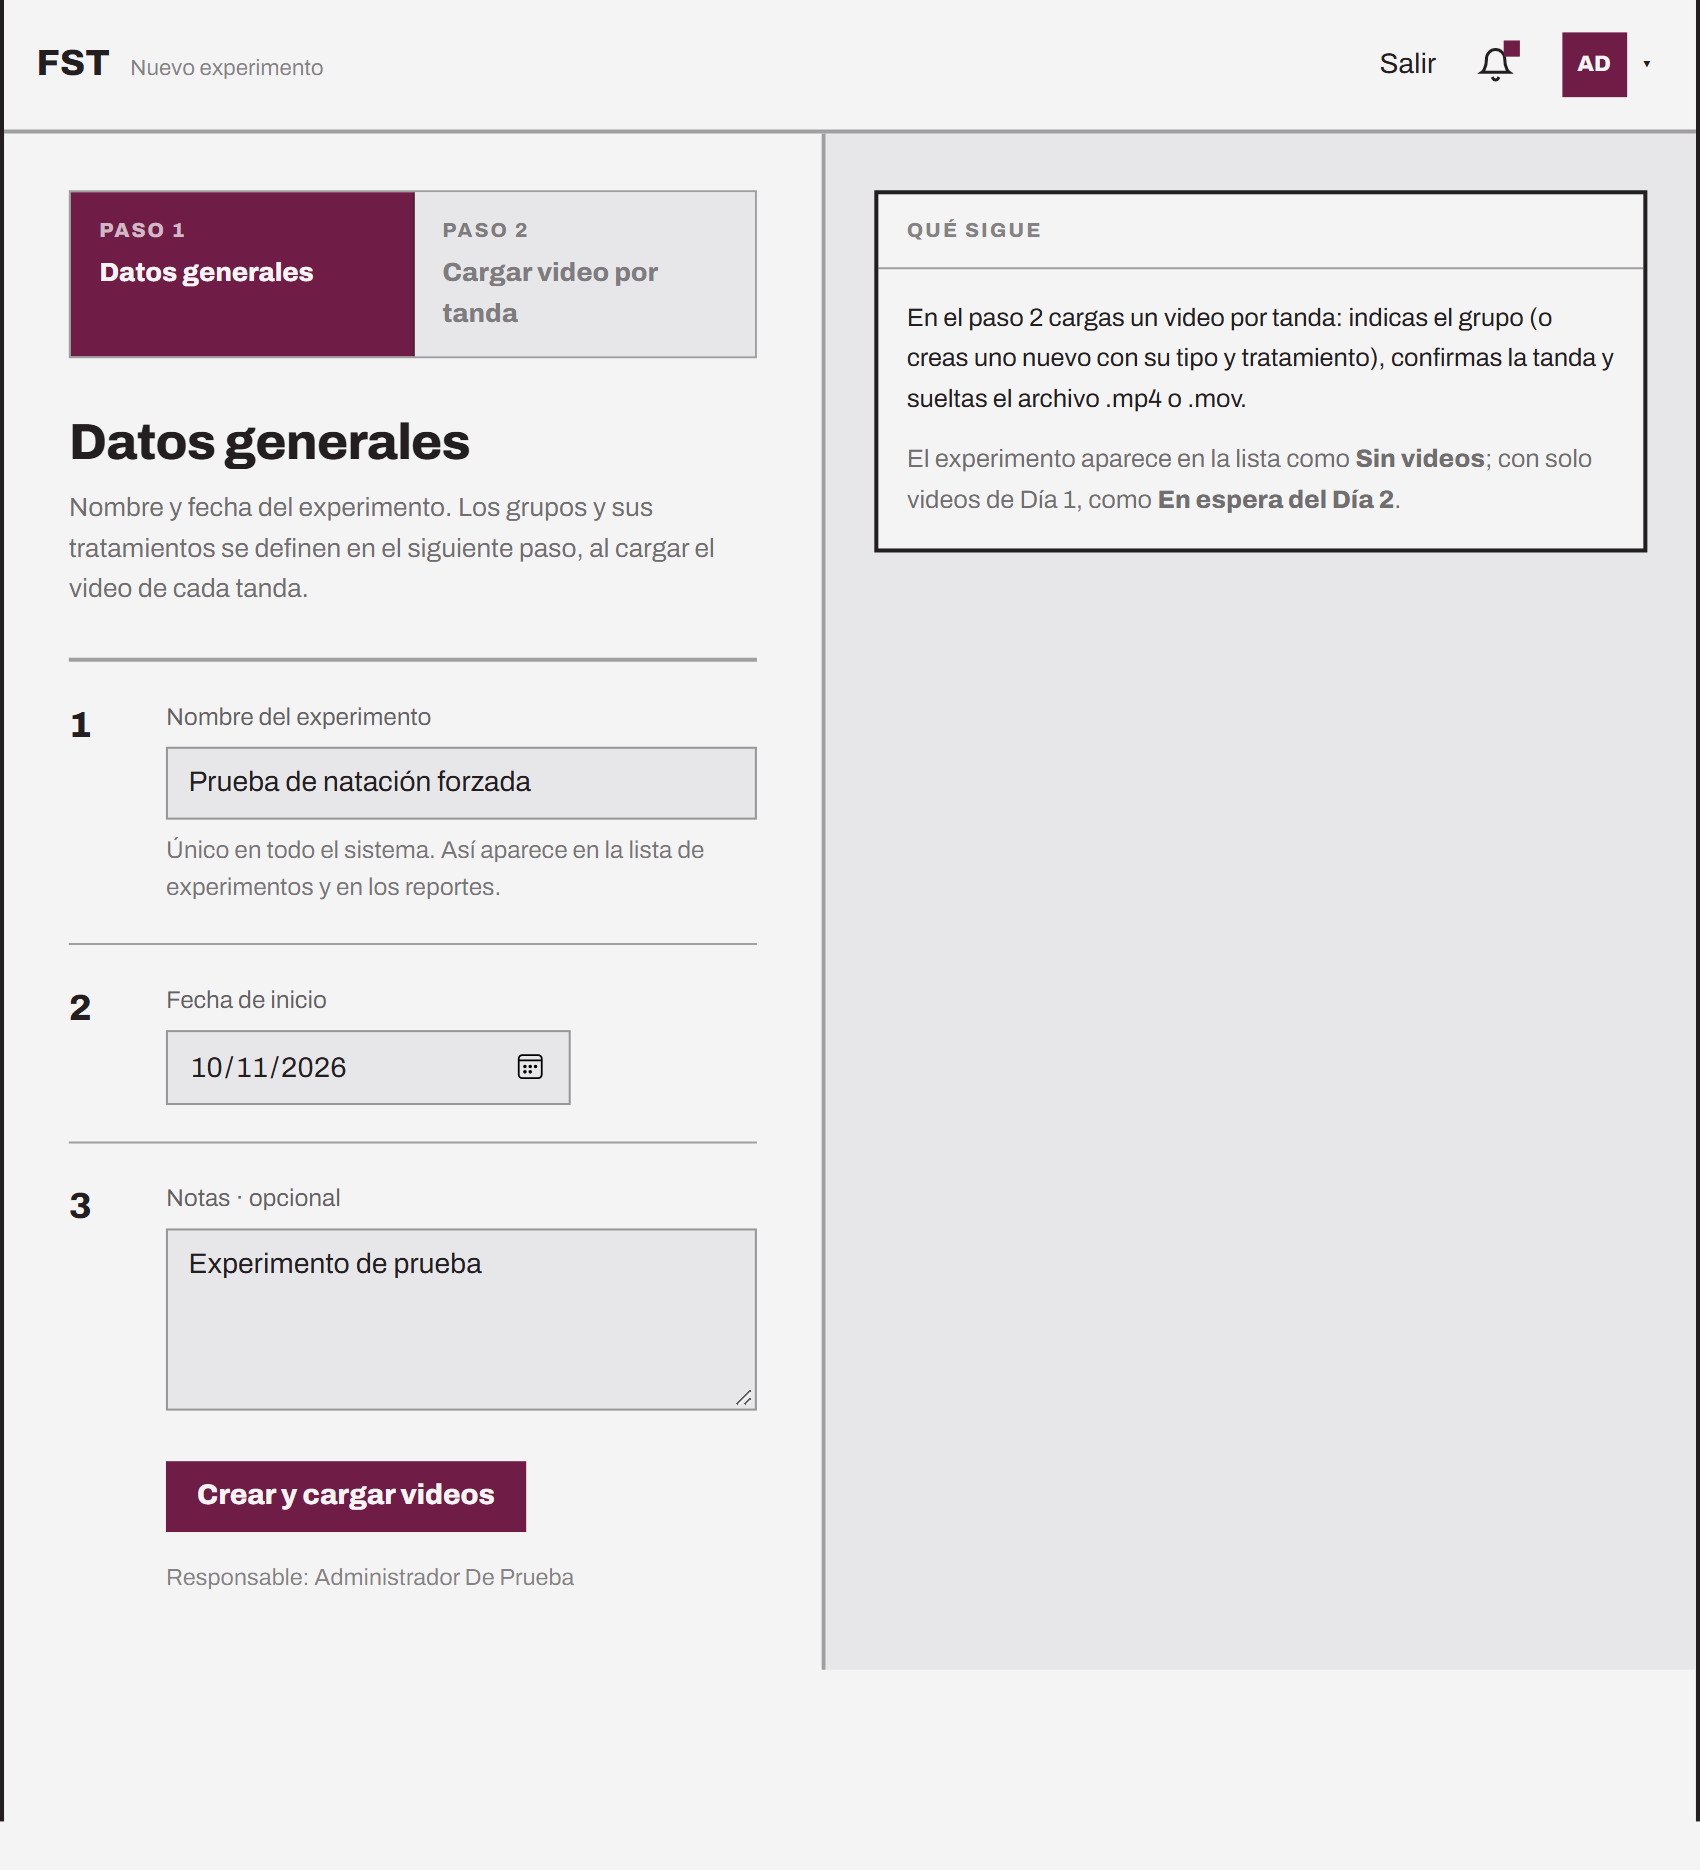
\includegraphics[width=17.5cm]{figures/pruebas/48_real_crear_experimento}}
\caption{Captura de la interfaz con el sistema completo: formulario para crear un experimento, con el responsable y las notas.}
\label{fig:pruebas_real_crear}
\end{figure}

\begin{figure}[tbp]
\centering
\makebox[\textwidth][c]{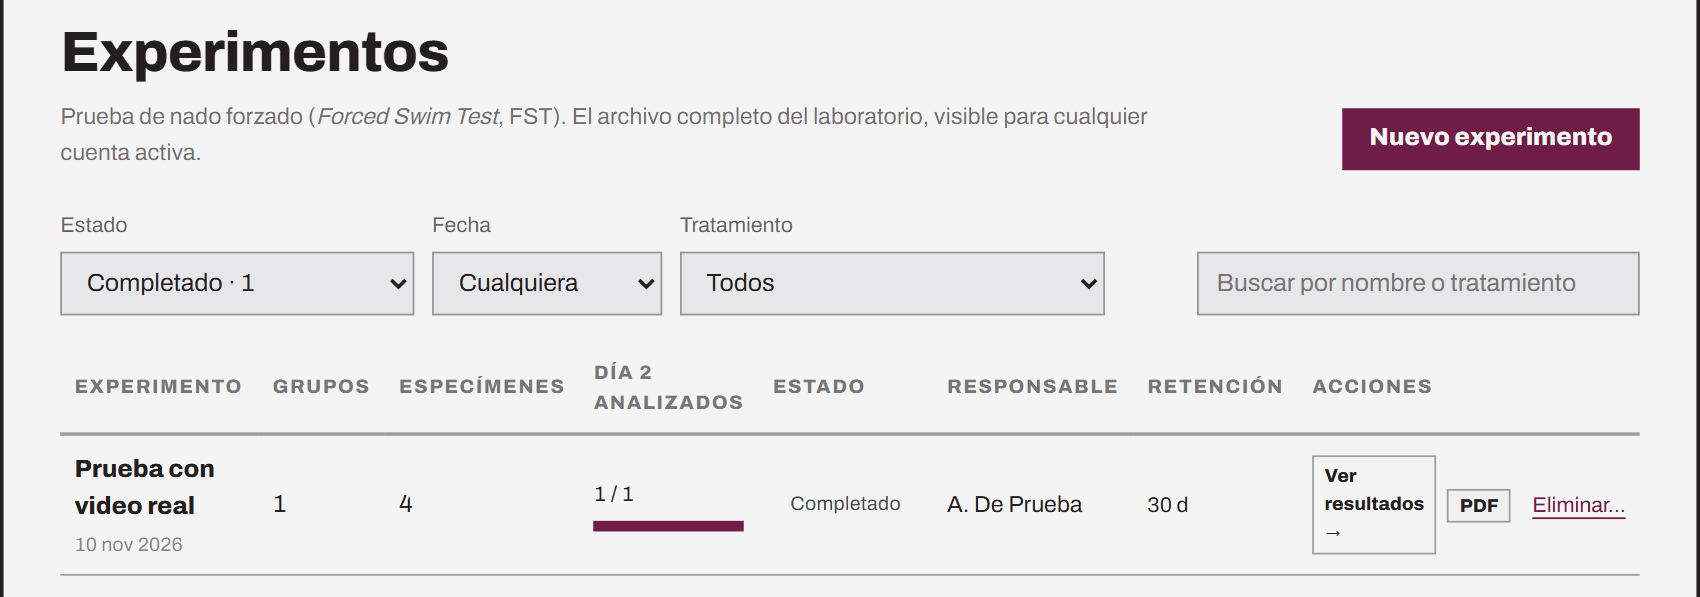
\includegraphics[width=19cm]{figures/pruebas/49_real_lista_de_experimentos_filtro_completado}}
\caption{Captura de la interfaz con el sistema completo: lista de experimentos con el filtro de estado «Completado».}
\label{fig:pruebas_real_lista}
\end{figure}

\FloatBarrier

\subsection{Reporte en PDF}

Las Figuras~\ref{fig:pruebas_real_pdf1} y \ref{fig:pruebas_real_pdf2} muestran las dos primeras
páginas del reporte en PDF que el sistema generó con el análisis real: los datos del experimento
y los resultados por grupo con una gráfica, y después la curva por minuto, la tabla por espécimen
y el desglose por minuto. La tercera página del reporte solo continúa el desglose.

\begin{figure}[tbp]
\centering
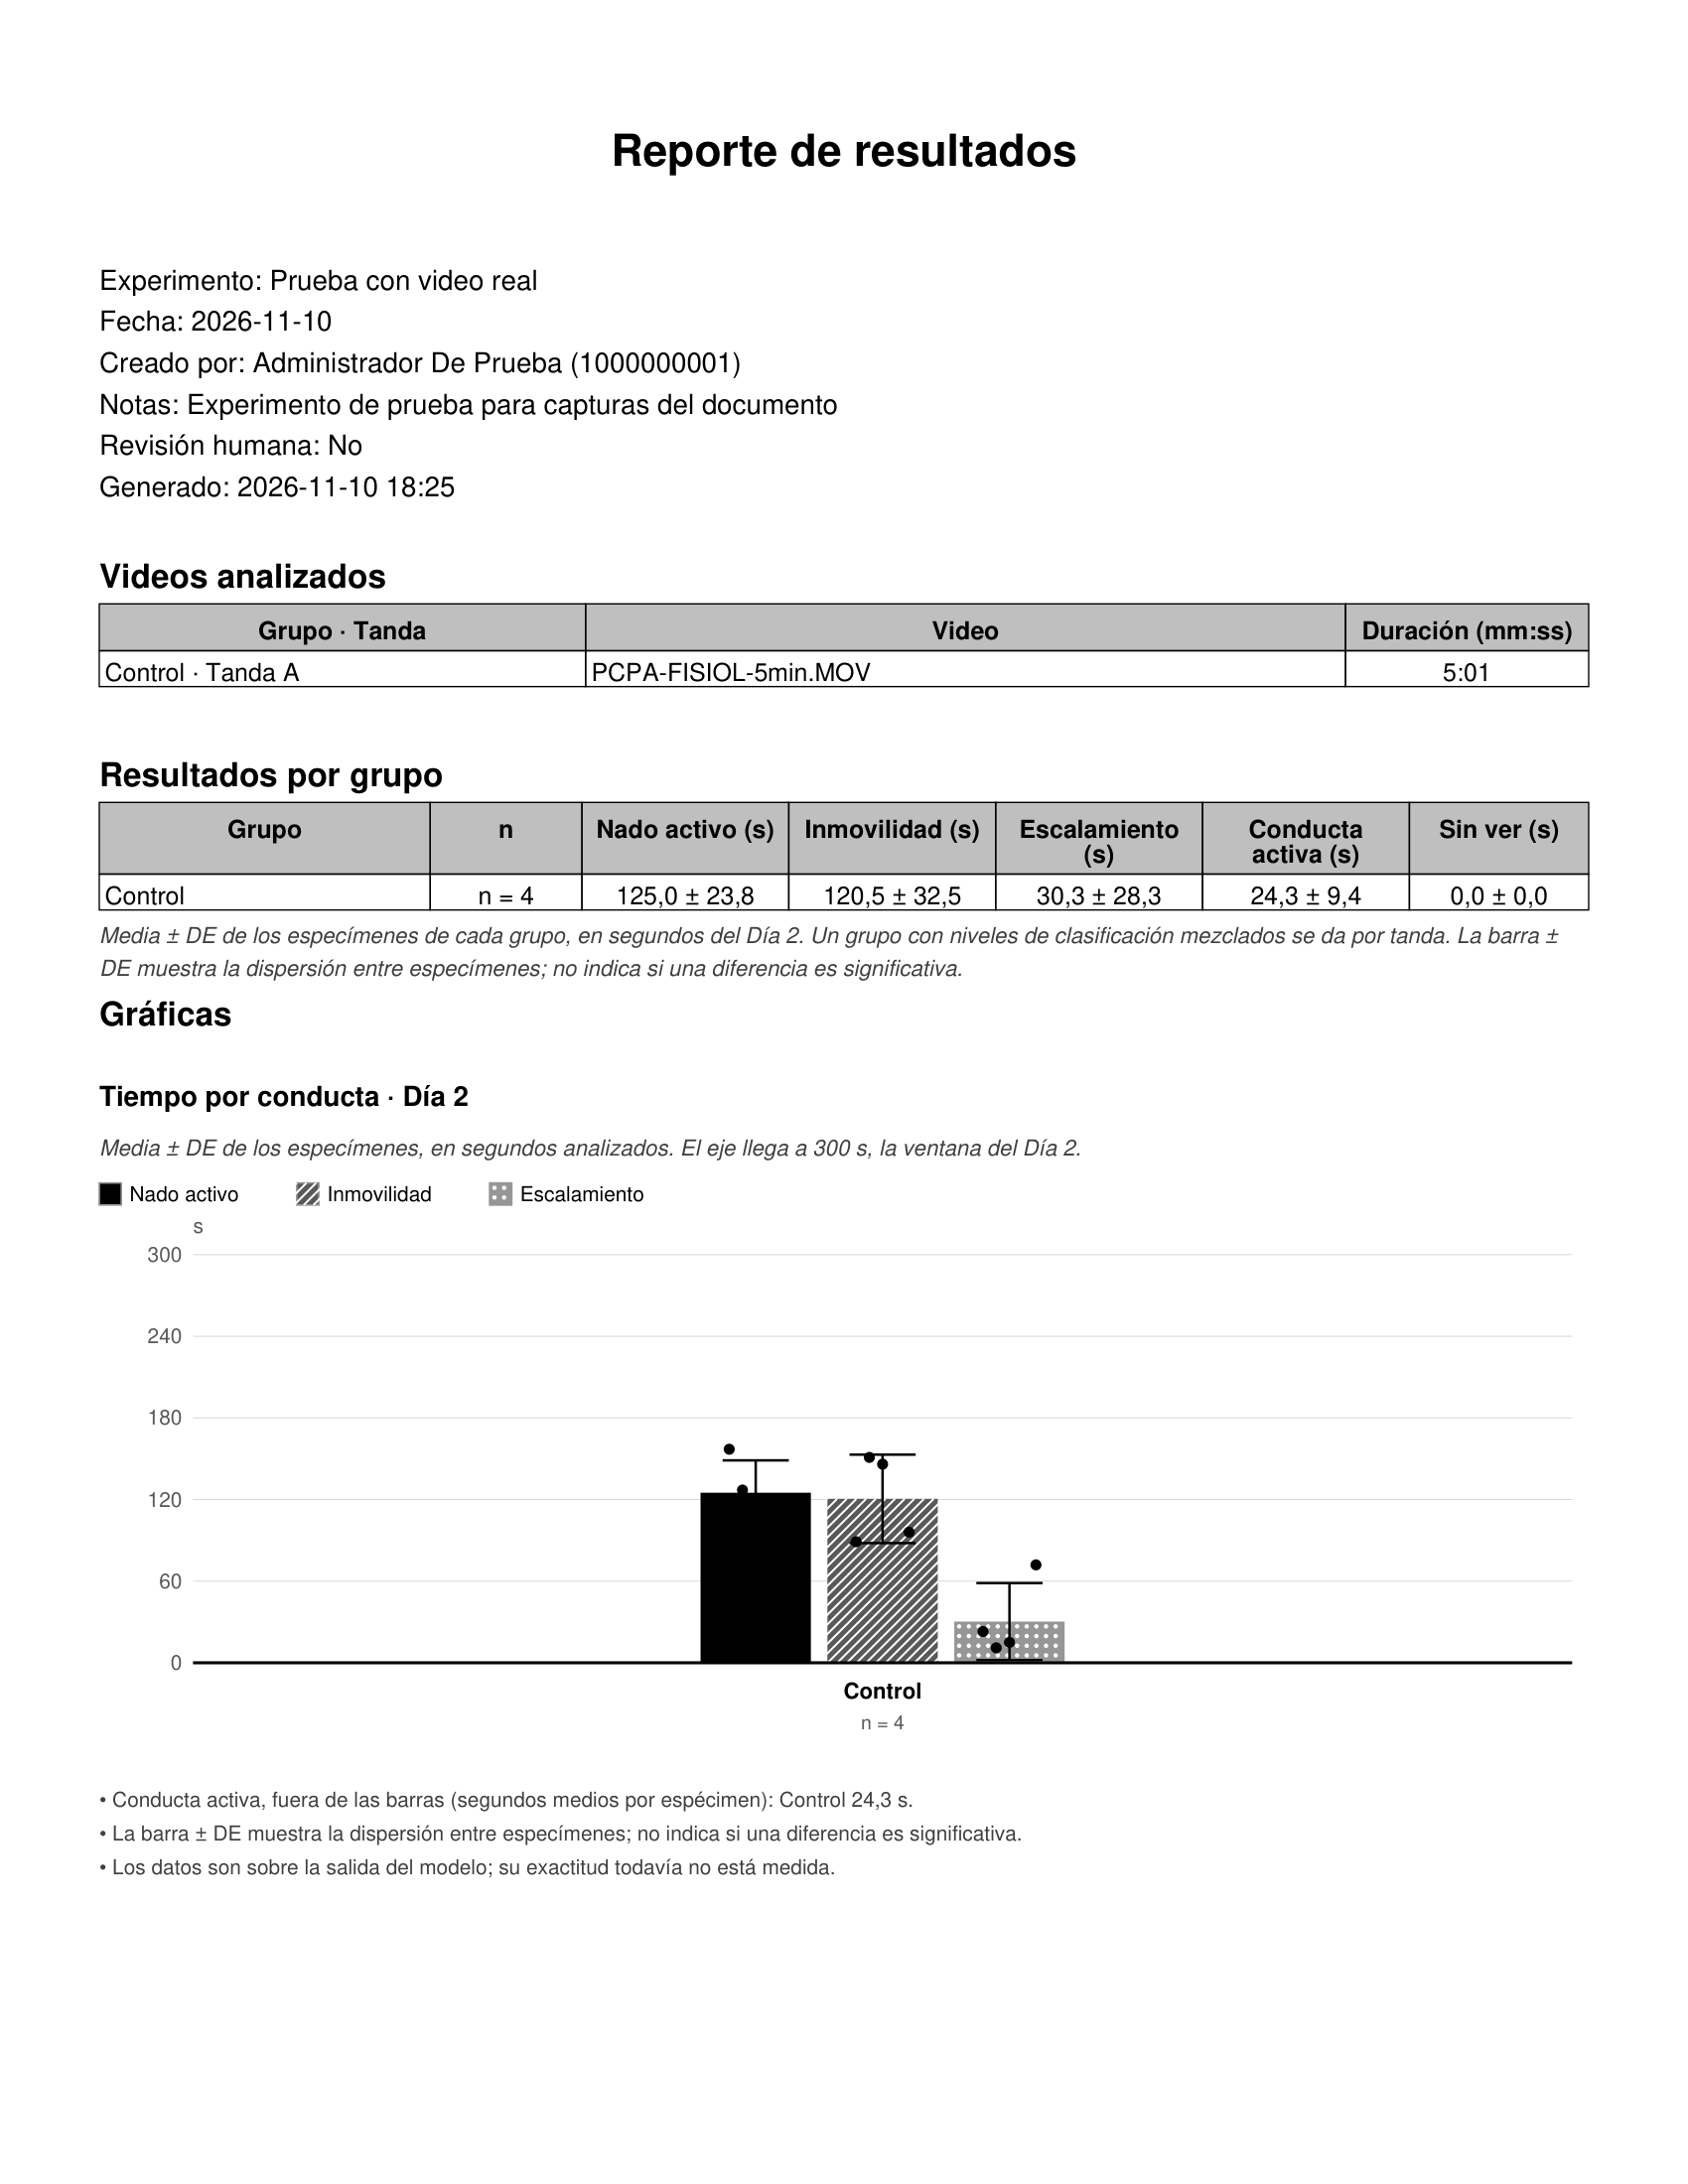
\includegraphics[width=0.8\textwidth]{figures/pruebas/45_real_reporte_pdf_pagina_1}
\caption{Reporte en PDF generado por el sistema con el análisis real: página 1.}
\label{fig:pruebas_real_pdf1}
\end{figure}

\begin{figure}[tbp]
\centering
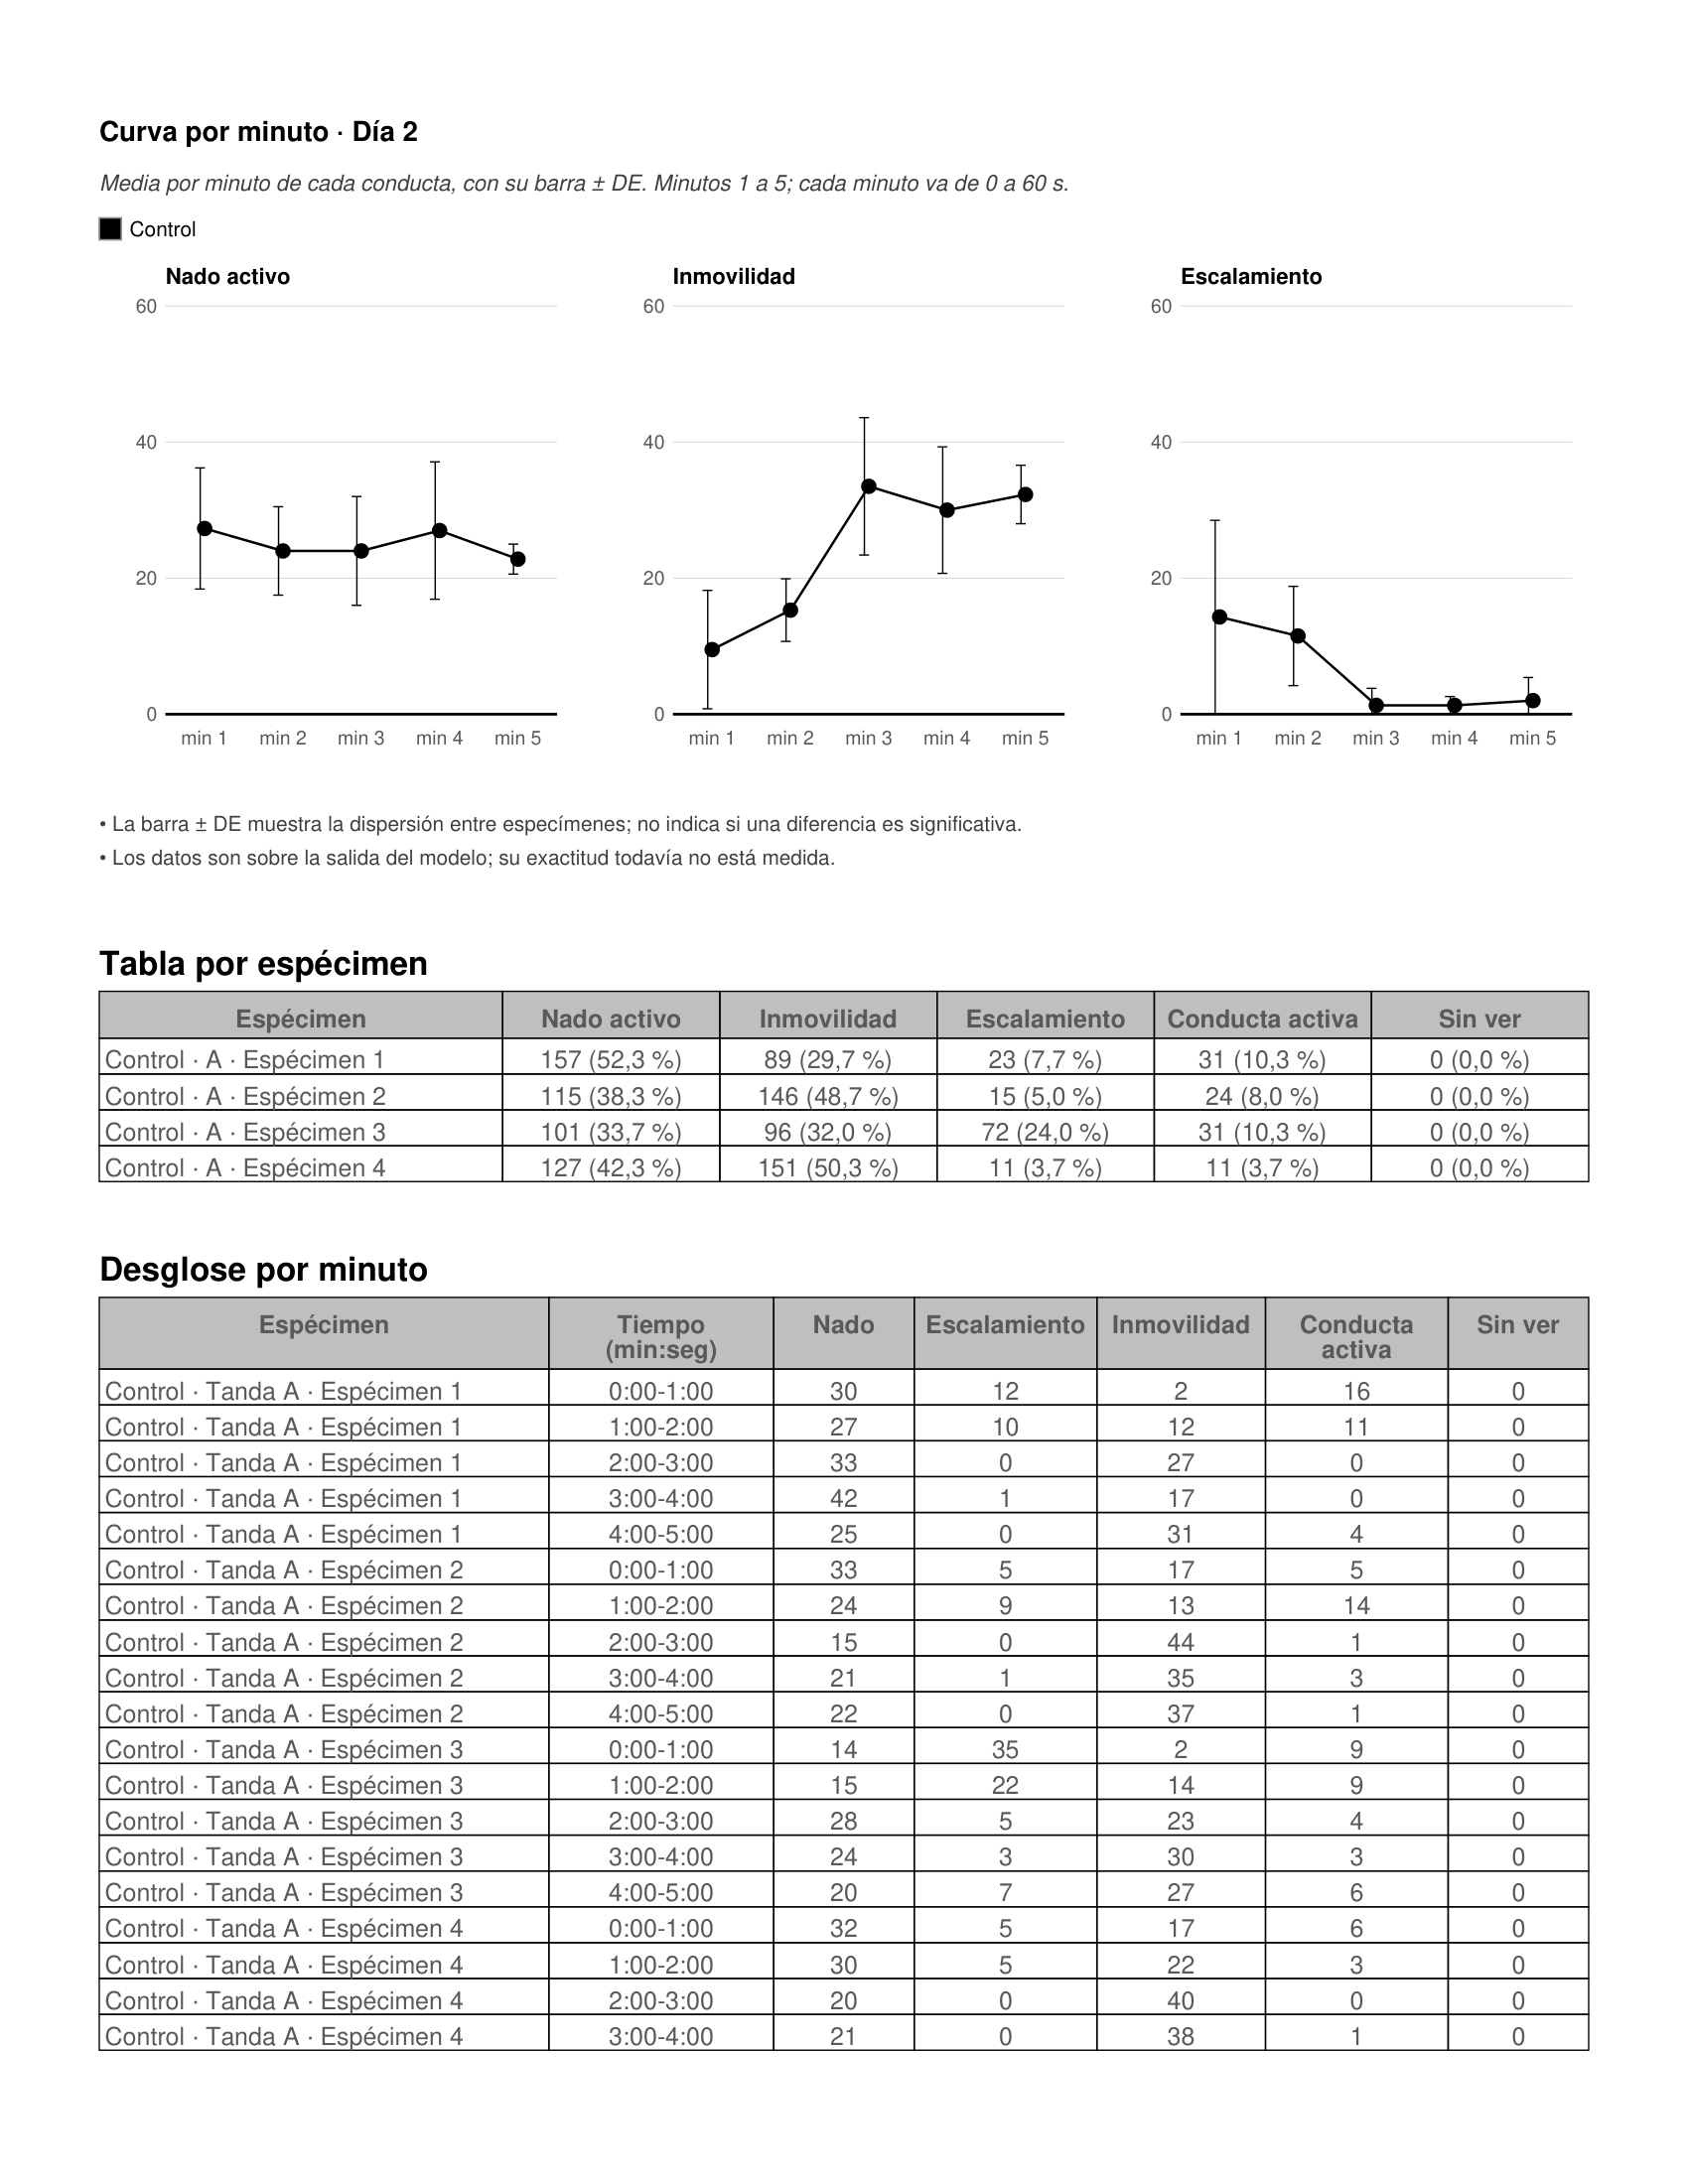
\includegraphics[width=0.8\textwidth]{figures/pruebas/45_real_reporte_pdf_pagina_2}
\caption{Reporte en PDF generado por el sistema con el análisis real: página 2.}
\label{fig:pruebas_real_pdf2}
\end{figure}

\FloatBarrier

% ============================================================
\section{Pantallas de otras funciones}
\label{sec:pruebas_pantallas}

Esta sección reúne capturas de la interfaz de las funciones que las pruebas de las secciones
anteriores verifican en el \textit{backend} y que no se capturaron con el sistema completo.
Son capturas del modo de ejemplo, un modo de la interfaz que corre sin servidor y con datos de
ejemplo. Ilustran cómo se ve cada función; no son resultado de las pruebas, que son del
\textit{backend}.

\subsection{Cuentas y sesión}

Las Figuras~\ref{fig:pruebas_login}, \ref{fig:pruebas_privacidad} y \ref{fig:pruebas_terminos}
muestran el inicio de sesión, el aviso de privacidad y los términos y condiciones de uso. La
Figura~\ref{fig:pruebas_primer_acceso} muestra el primer acceso de una cuenta con contraseña
temporal, que exige aceptar ambos textos, y la Figura~\ref{fig:pruebas_recuperar} la
solicitud del enlace para recuperar la contraseña. Son las pantallas de las funciones que
verifican las pruebas de seguridad.

\begin{figure}[tbp]
\centering
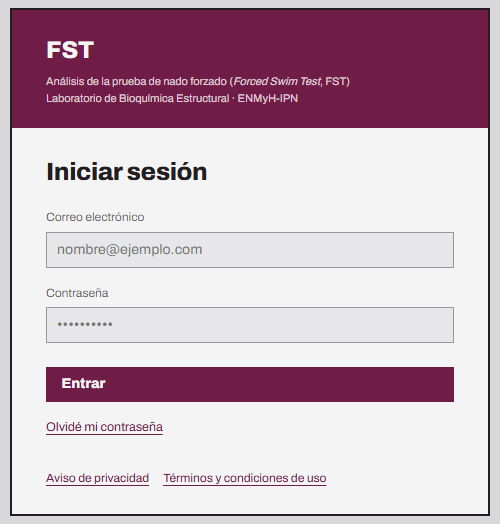
\includegraphics[width=0.7\textwidth]{figures/pruebas/07_pantalla_inicio_de_sesion}
\caption{Captura de la interfaz en modo de ejemplo (sin servidor): pantalla de inicio de sesión, con los enlaces al aviso de privacidad y a los términos y condiciones de uso.}
\label{fig:pruebas_login}
\end{figure}

\begin{figure}[tbp]
\centering
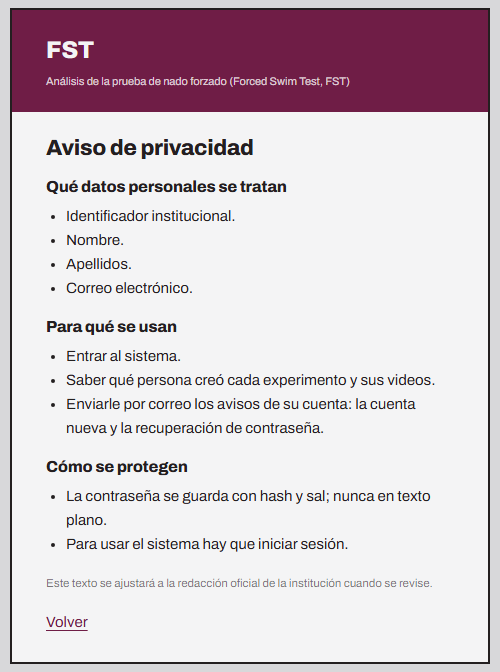
\includegraphics[width=0.7\textwidth]{figures/pruebas/08_pantalla_aviso_de_privacidad}
\caption{Captura de la interfaz en modo de ejemplo (sin servidor): aviso de privacidad.}
\label{fig:pruebas_privacidad}
\end{figure}

\begin{figure}[tbp]
\centering
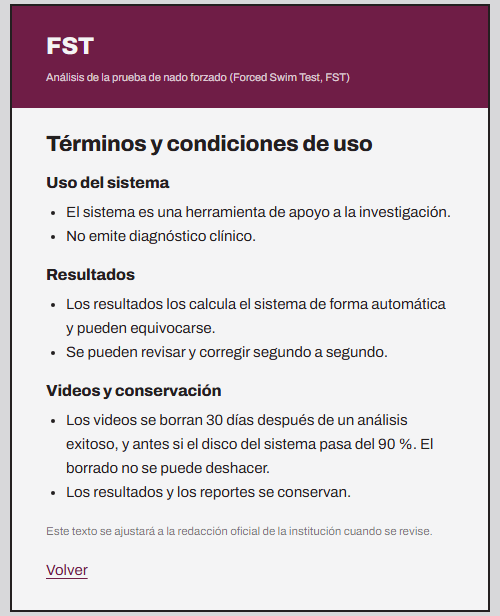
\includegraphics[width=0.7\textwidth]{figures/pruebas/09_pantalla_terminos_y_condiciones}
\caption{Captura de la interfaz en modo de ejemplo (sin servidor): términos y condiciones de uso.}
\label{fig:pruebas_terminos}
\end{figure}

\begin{figure}[tbp]
\centering
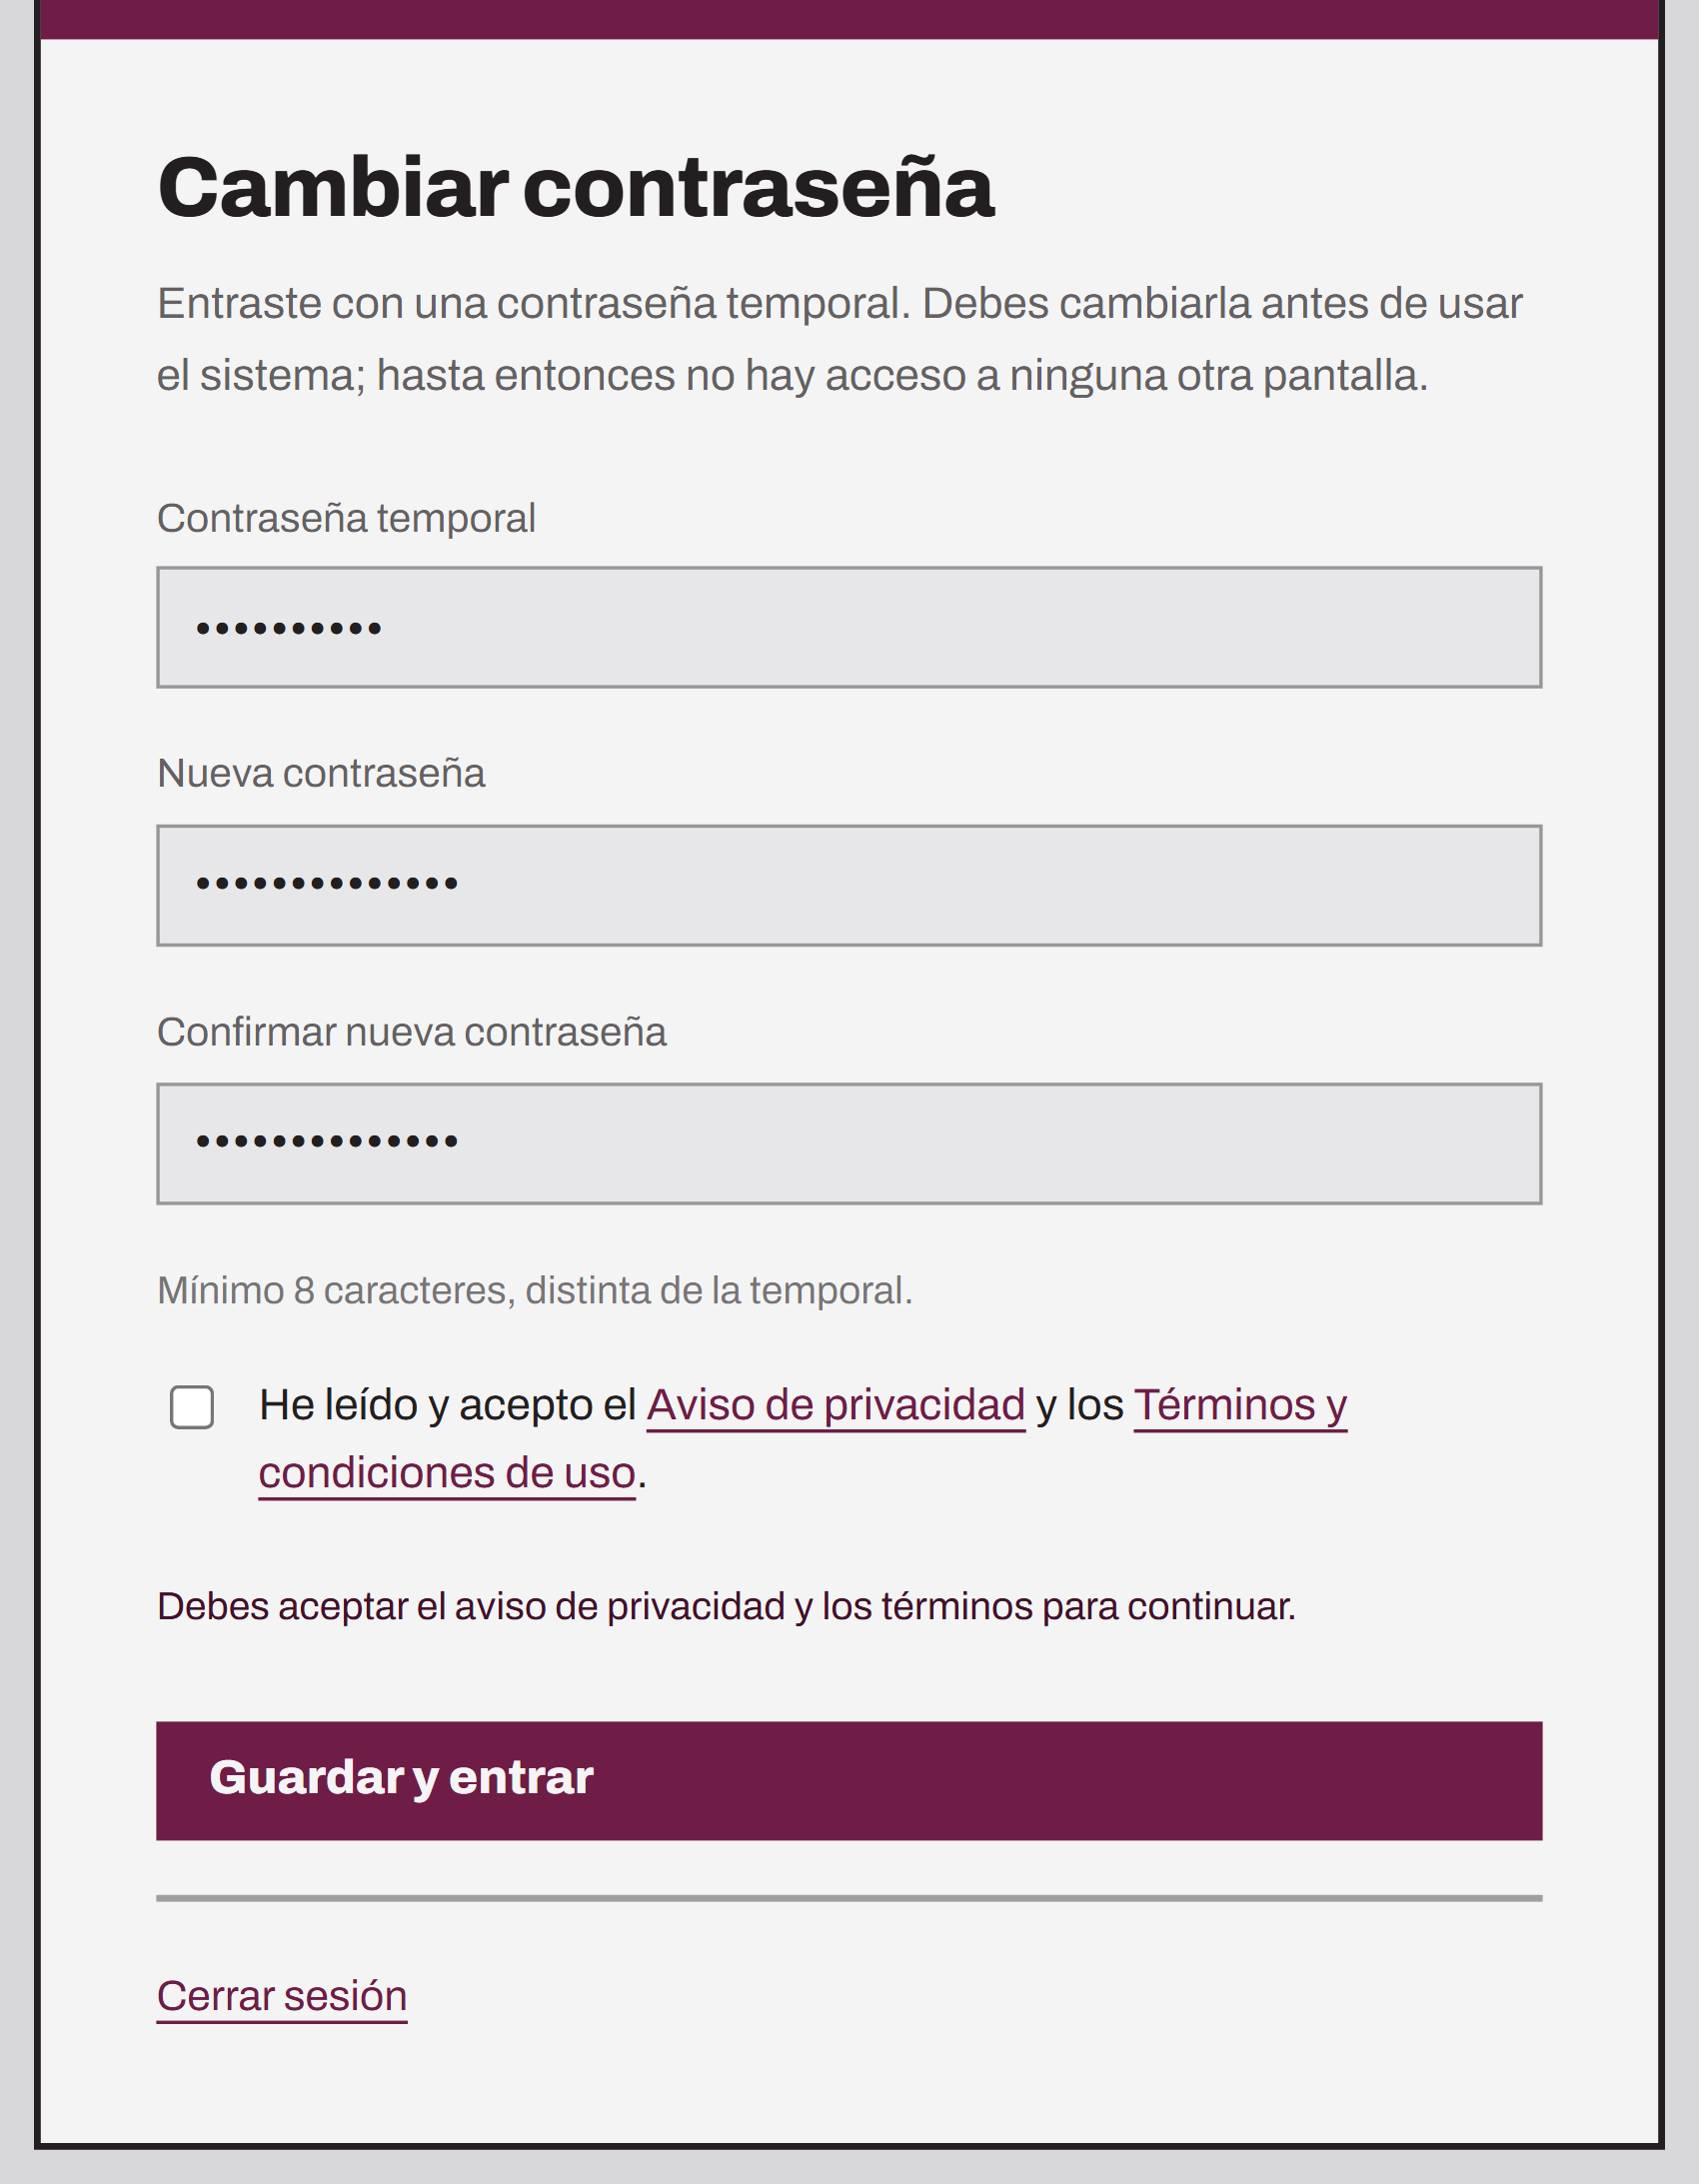
\includegraphics[width=0.7\textwidth]{figures/pruebas/12_primer_acceso_sin_aceptar_terminos}
\caption{Captura de la interfaz en modo de ejemplo (sin servidor): primer acceso con contraseña temporal. La casilla de aceptación del aviso de privacidad y los términos está sin marcar y la pantalla pide aceptarlos para continuar.}
\label{fig:pruebas_primer_acceso}
\end{figure}

\begin{figure}[tbp]
\centering
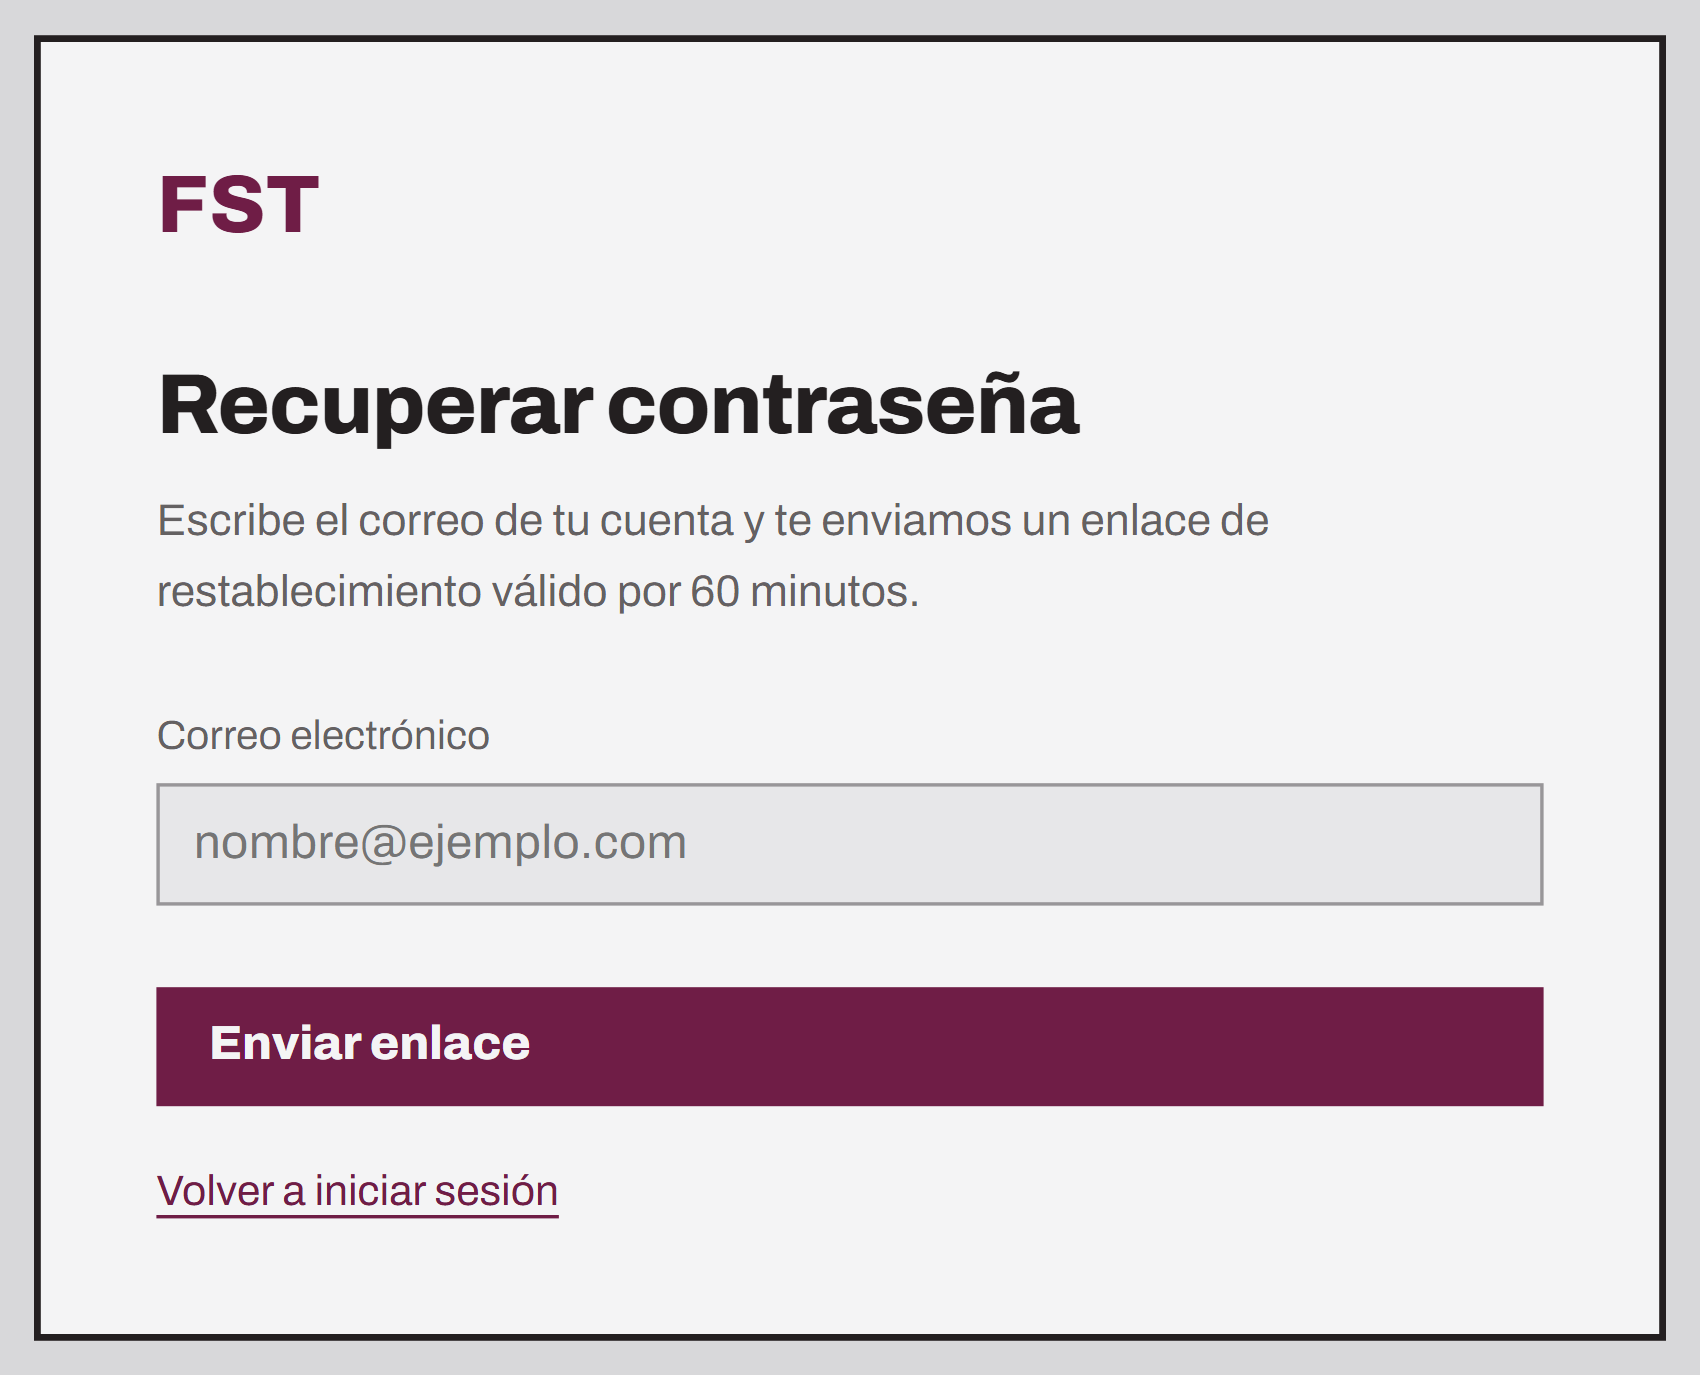
\includegraphics[width=0.7\textwidth]{figures/pruebas/13_recuperar_contrasena}
\caption{Captura de la interfaz en modo de ejemplo (sin servidor): recuperación de contraseña, donde se pide el correo para recibir el enlace de restablecimiento.}
\label{fig:pruebas_recuperar}
\end{figure}

\FloatBarrier

\subsection{Experimentos}

La Figura~\ref{fig:pruebas_carga_a} y su continuación (Figura~\ref{fig:pruebas_carga_b}) muestran la
carga de video por tanda, con el botón para agregar otra tanda. La
Figura~\ref{fig:pruebas_eliminar} muestra la confirmación que se pide antes de eliminar un
experimento.

\begin{figure}[tbp]
\centering
\makebox[\textwidth][c]{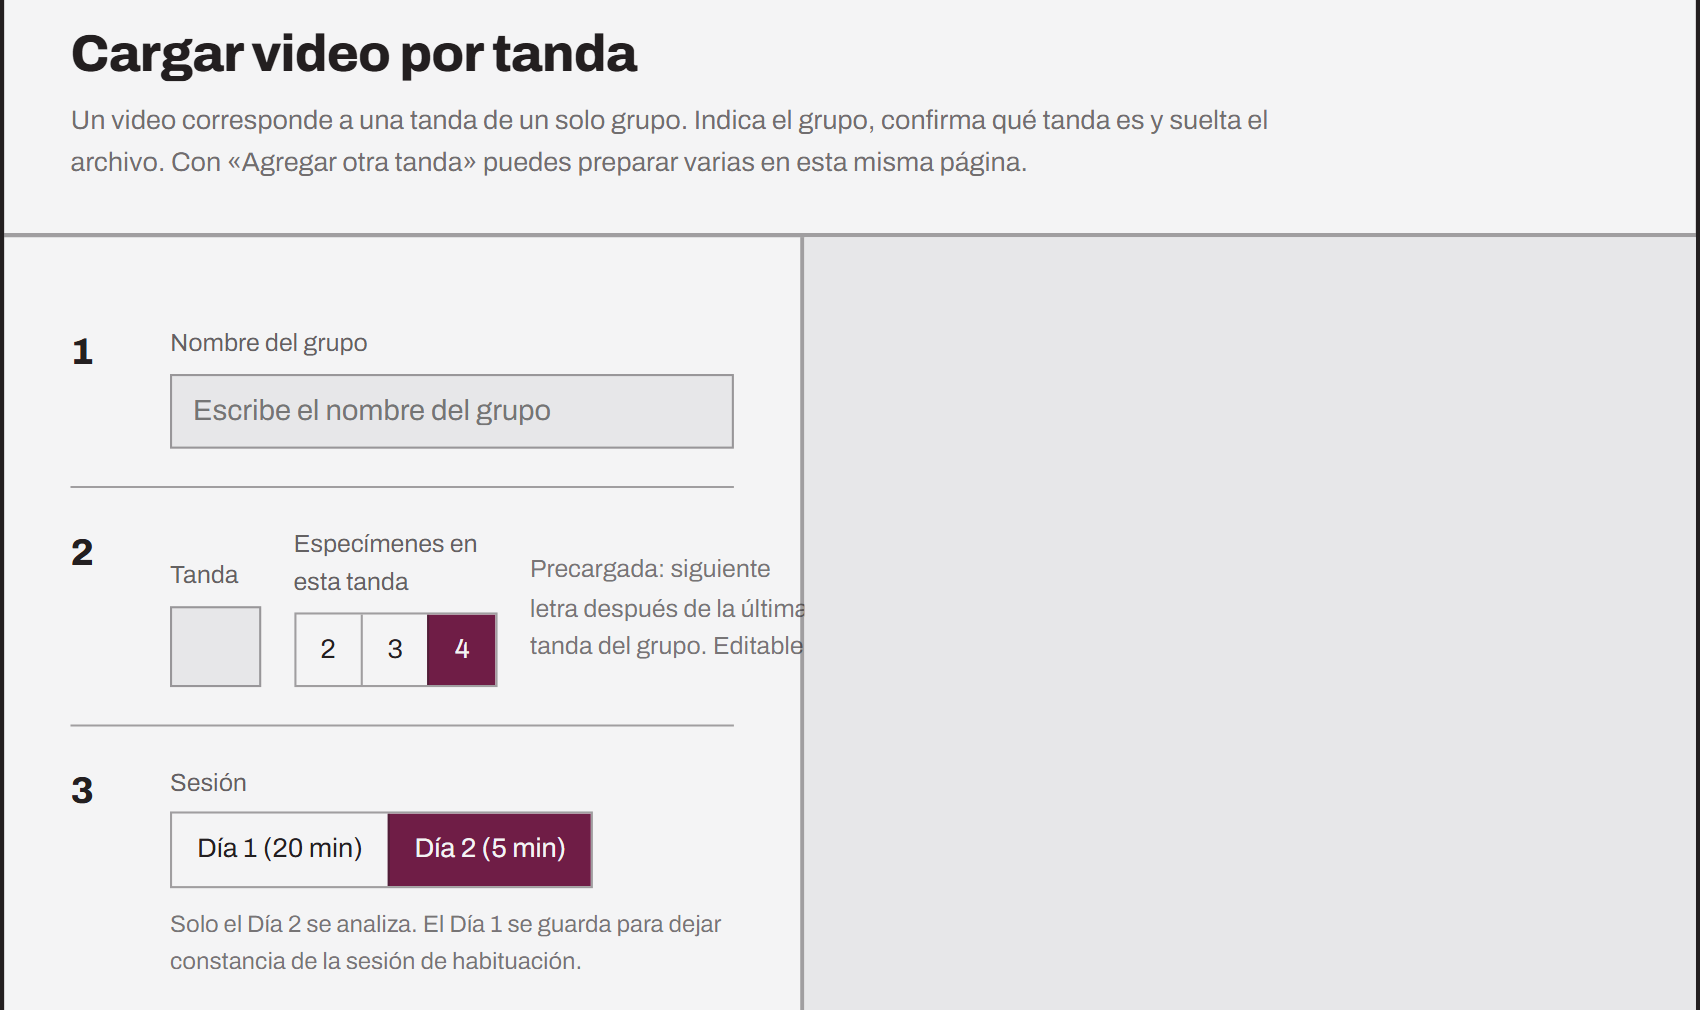
\includegraphics[width=17cm]{figures/pruebas/15_cargar_video_por_tanda_a}}
\caption{Captura de la interfaz en modo de ejemplo (sin servidor): carga de video por tanda, con el grupo, la tanda y la sesión.}
\label{fig:pruebas_carga_a}
\end{figure}

\begin{figure}[tbp]
\ContinuedFloat
\centering
\makebox[\textwidth][c]{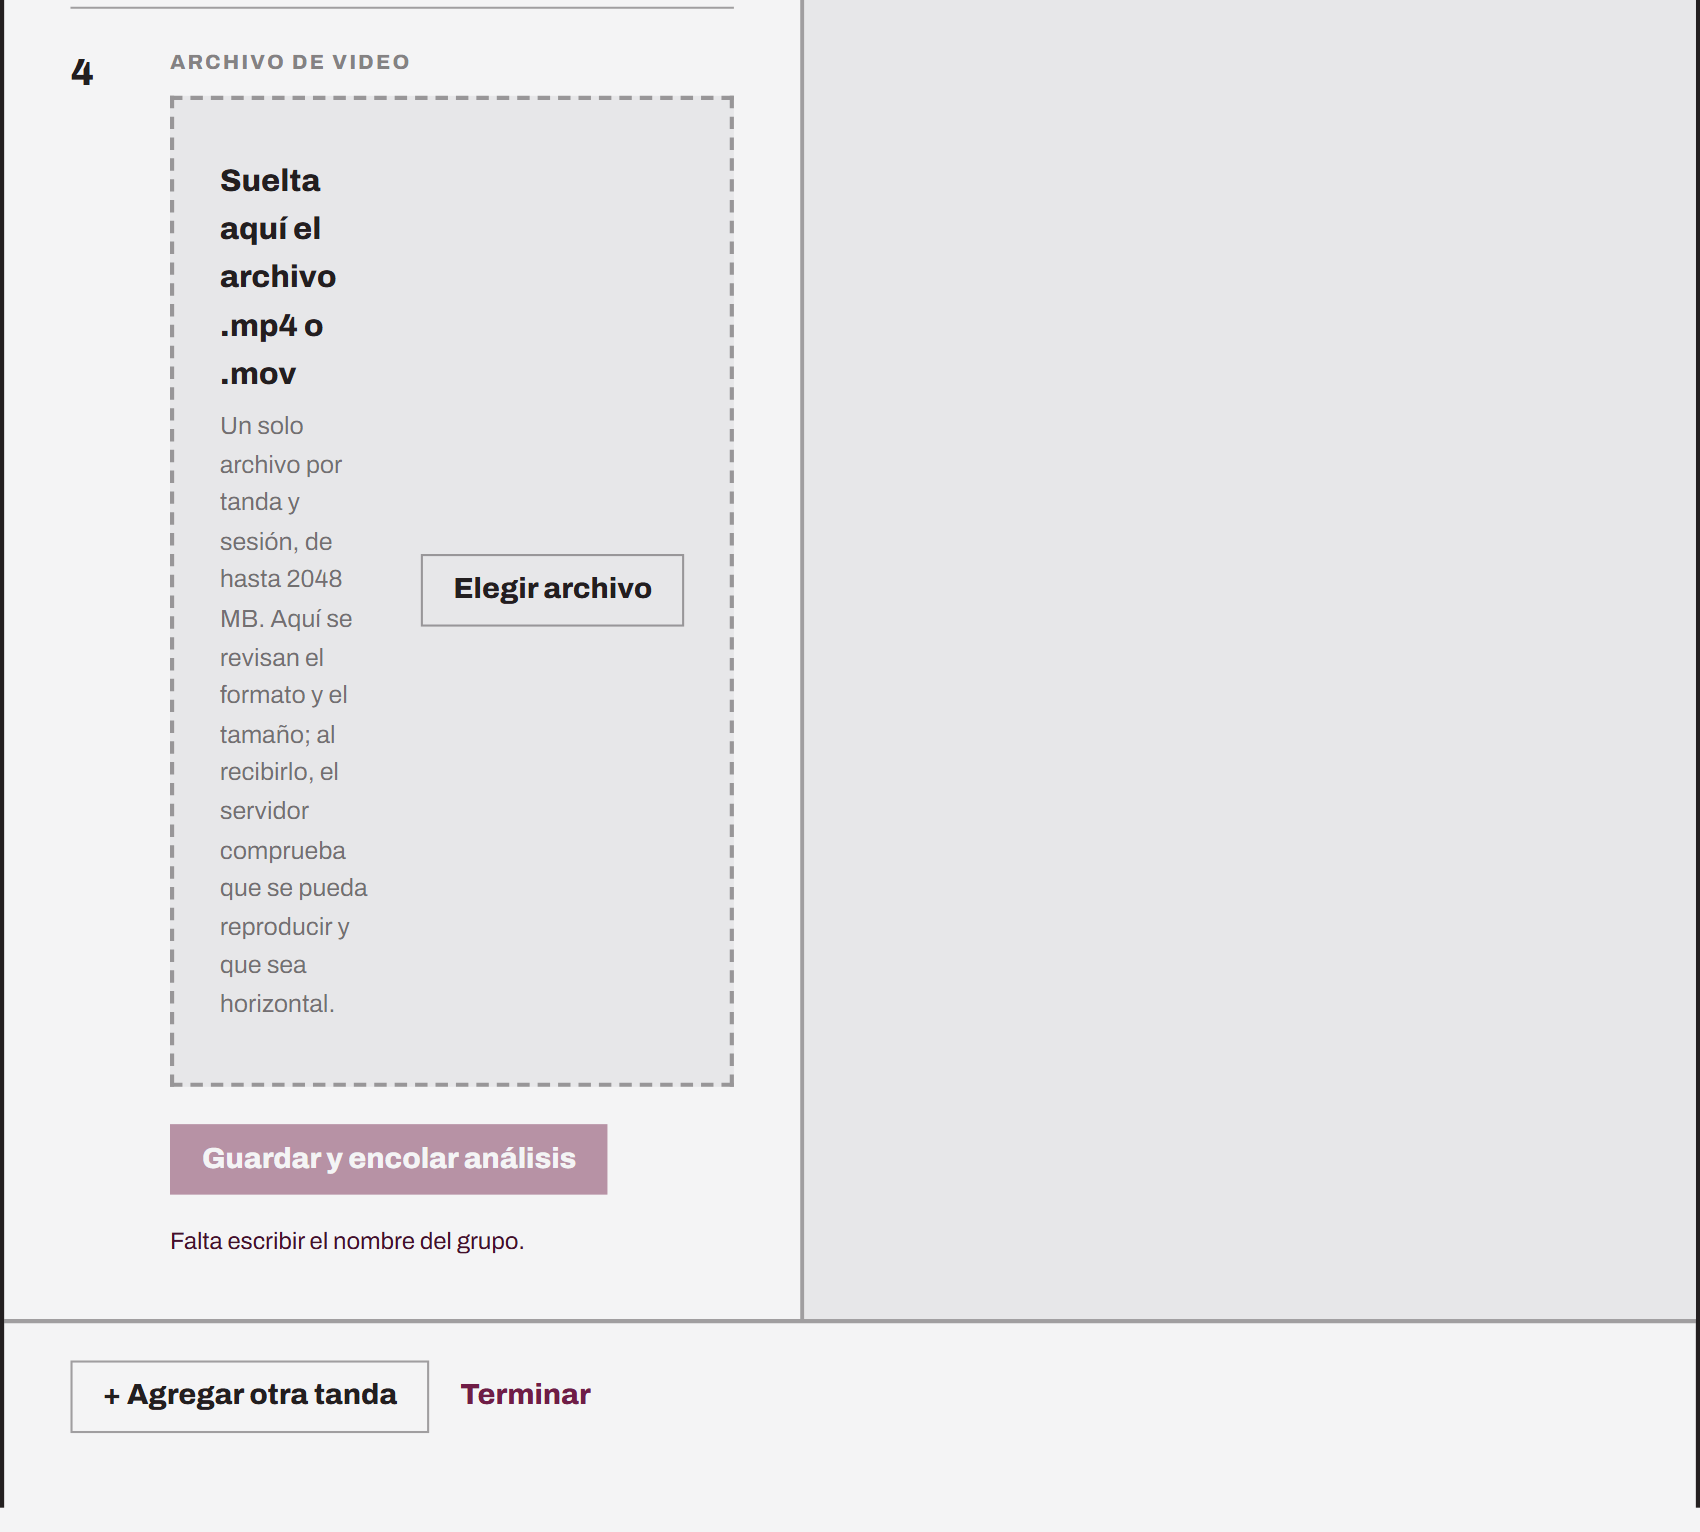
\includegraphics[width=17cm]{figures/pruebas/15_cargar_video_por_tanda_b}}
\caption[]{Captura de la interfaz en modo de ejemplo (sin servidor): carga de video por tanda, con el archivo de video y el botón para agregar otra tanda (continuación).}
\label{fig:pruebas_carga_b}
\end{figure}

\begin{figure}[tbp]
\centering
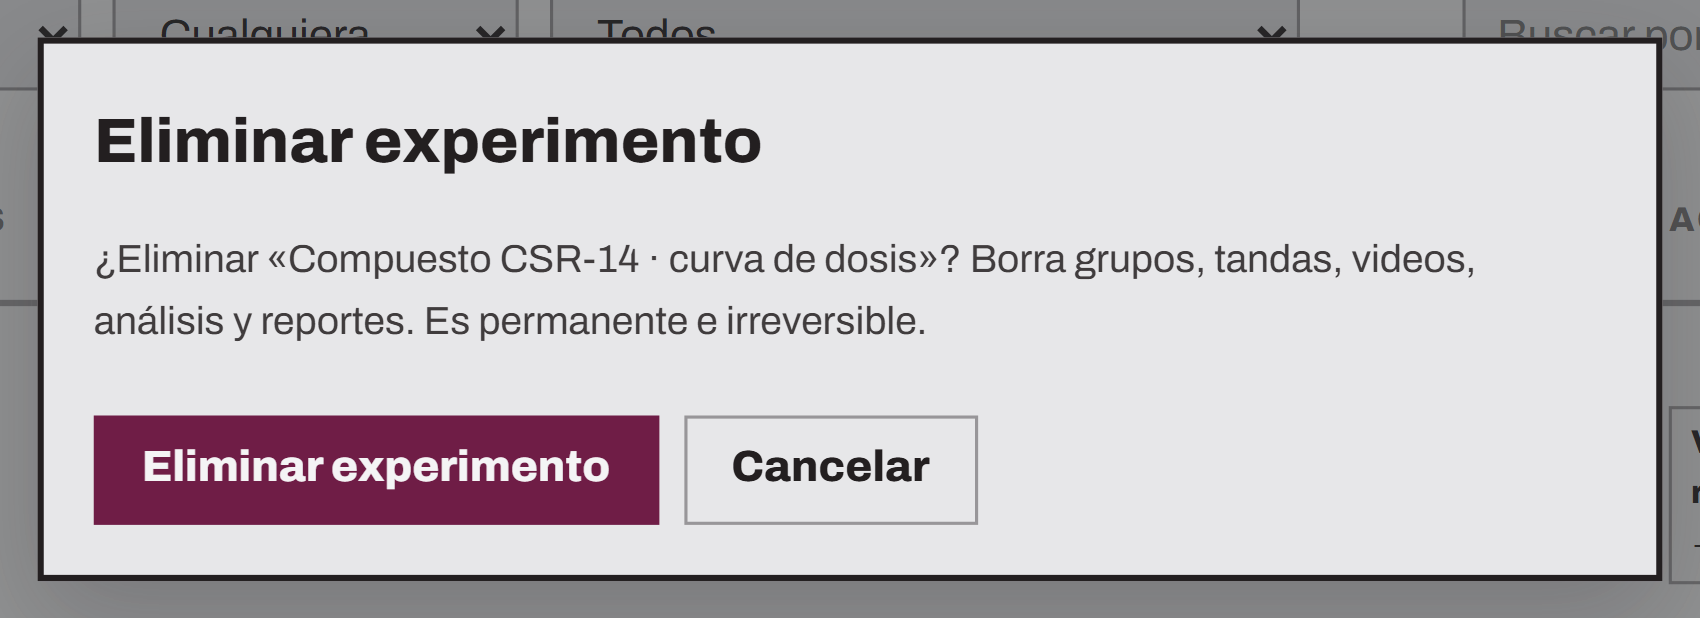
\includegraphics[width=0.75\textwidth]{figures/pruebas/17_confirmar_eliminar_experimento}
\caption{Captura de la interfaz en modo de ejemplo (sin servidor): confirmación antes de eliminar un experimento.}
\label{fig:pruebas_eliminar}
\end{figure}

\FloatBarrier

\subsection{Pausa}

La Figura~\ref{fig:pruebas_pausa} muestra la pantalla de un análisis en pausa, con el cilindro
que se dejó de ver, el segundo, el tiempo para responder y los tres botones. El modo de ejemplo
muestra un aviso en lugar de la imagen del instante; los recuadros sí se pueden ajustar.

\begin{figure}[tbp]
\centering
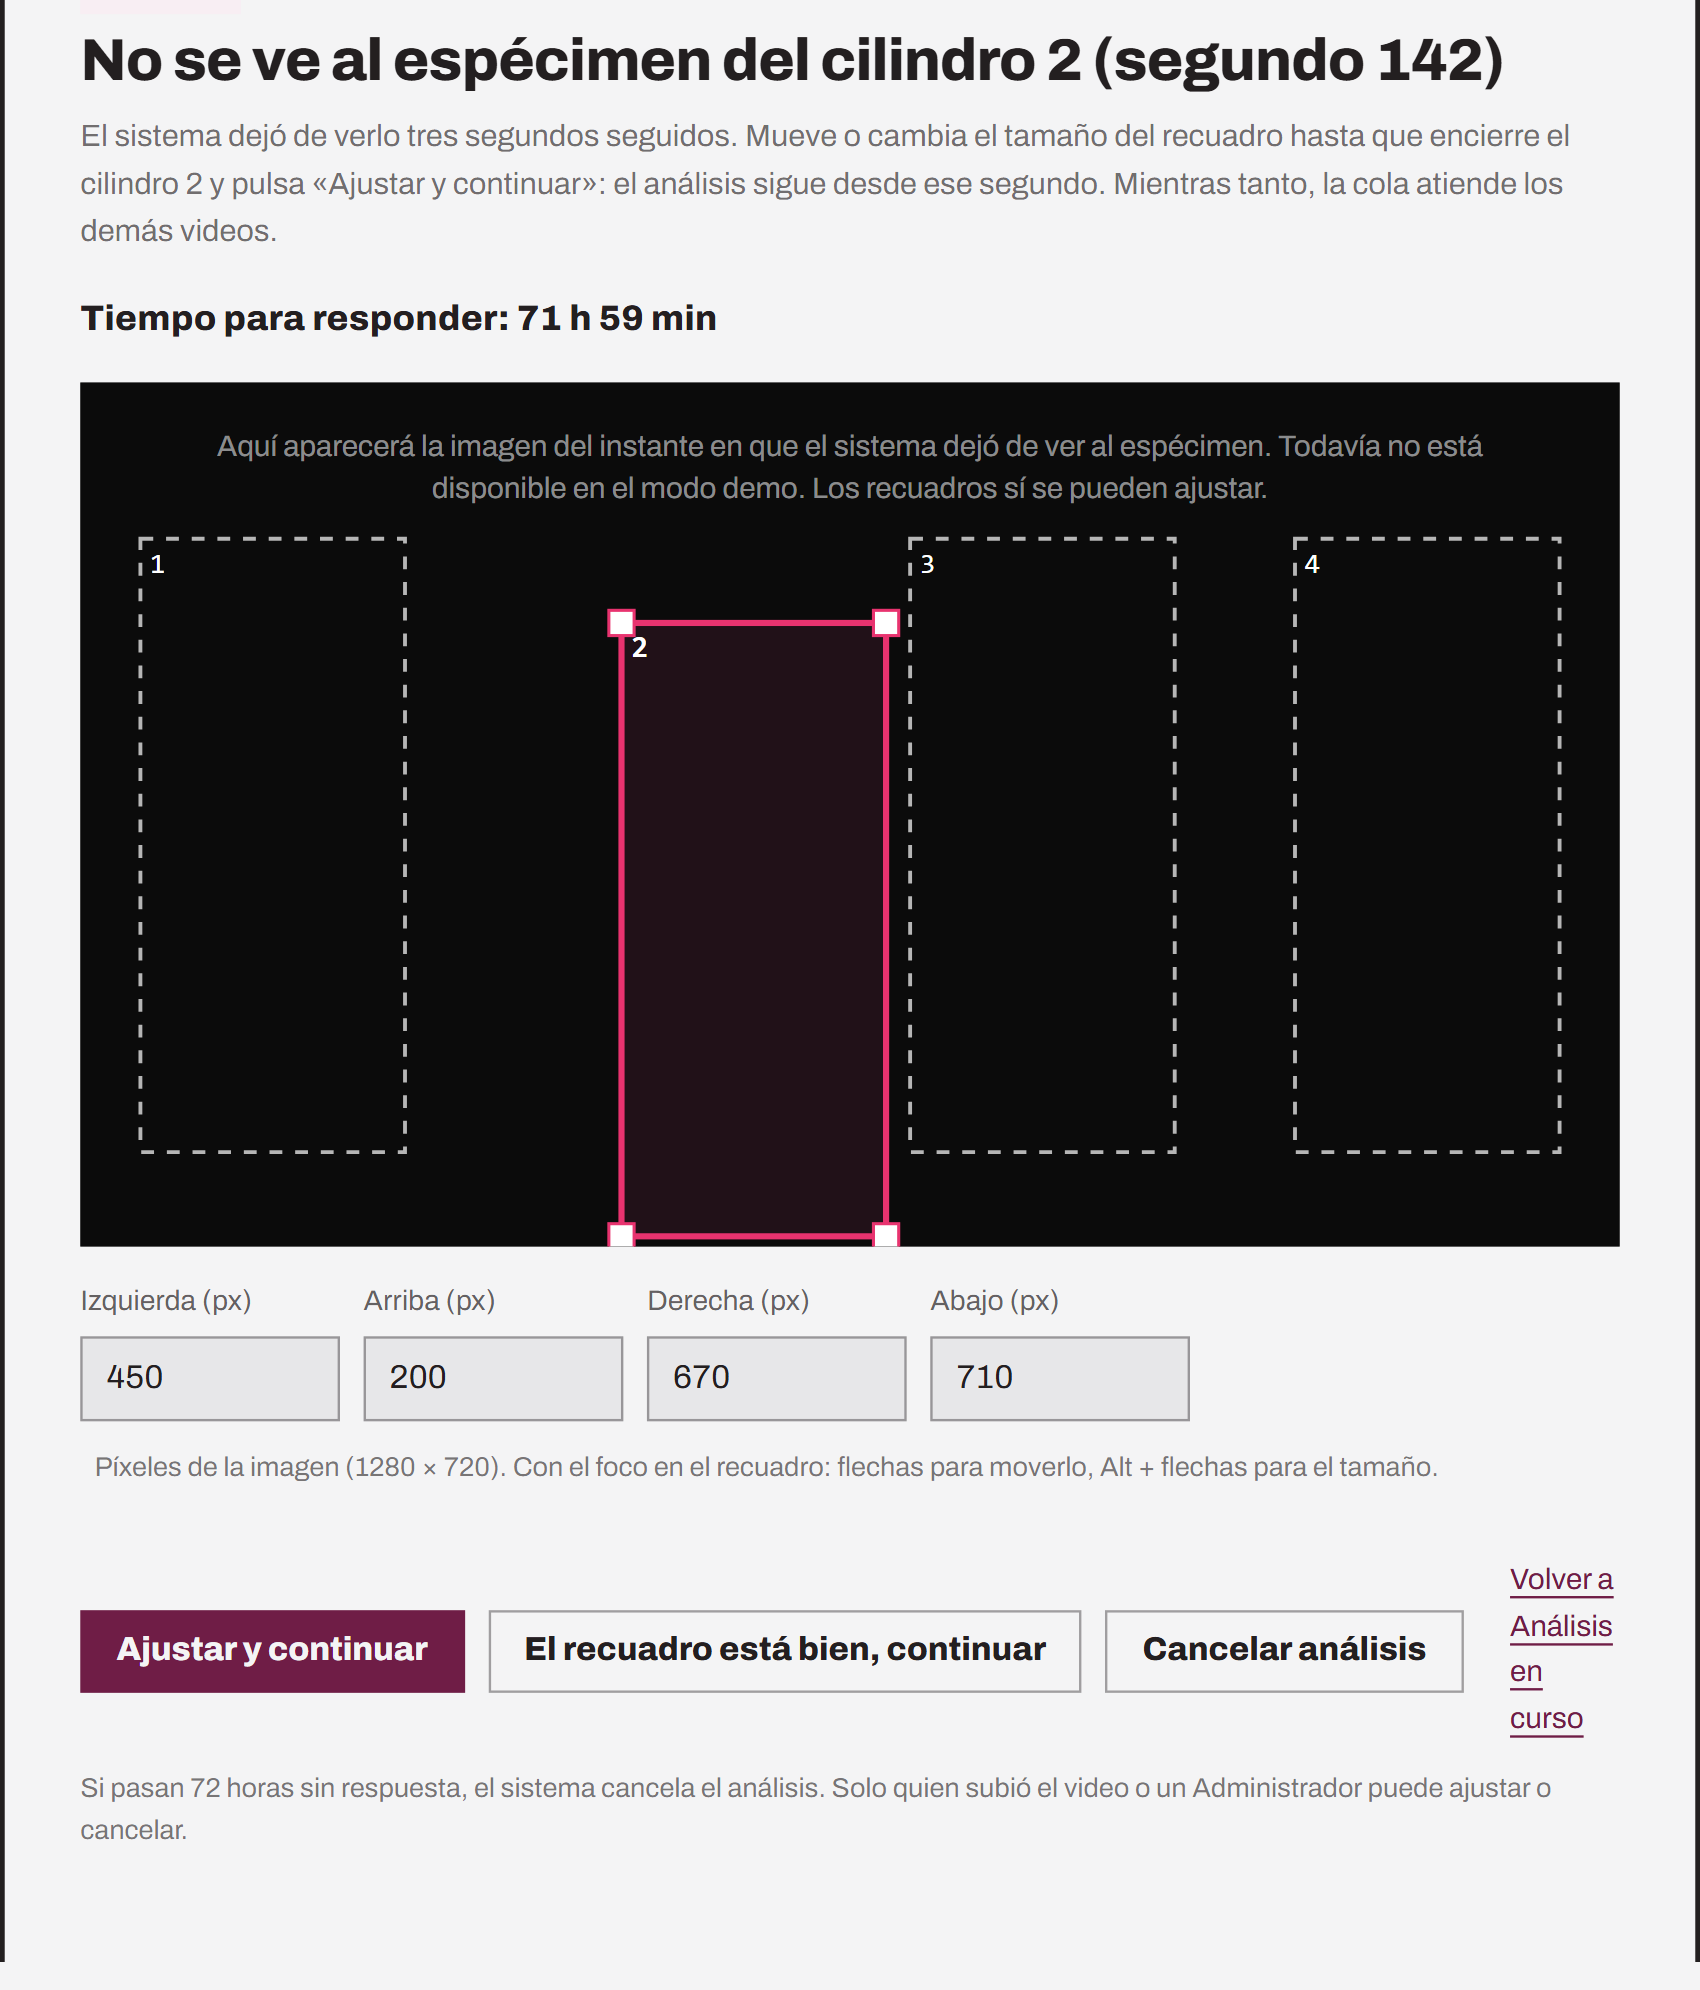
\includegraphics[width=0.9\textwidth]{figures/pruebas/18_pantalla_de_pausa}
\caption{Captura de la interfaz en modo de ejemplo (sin servidor): análisis en pausa, con el cilindro, el segundo, el plazo para responder y los botones. Sin imagen real del instante.}
\label{fig:pruebas_pausa}
\end{figure}

\FloatBarrier

% ============================================================
\section{Alcance y límites de las pruebas}
\label{sec:pruebas_limites}

La selección verifica reglas de negocio de cuentas, experimentos, resultados y revisión
contra una base real, y la integridad del esquema. No verifica todo el sistema. En
particular, no cubre:

\begin{itemize}
  \item el ajuste del recuadro y el botón «continuar» de la pausa; solo se comprueba el
        estado del análisis cuando está en pausa;
  \item un video que \textit{ffprobe} (la herramienta que lee las propiedades de un video)
        no puede leer;
  \item la subida de un video con un tipo de grupo o una sesión inválidos; solo se
        comprueban el archivo que no es MP4 ni MOV y el video vertical;
  \item la conservación de los resultados y el borrado automático a los 30 días;
  \item la clasificación de conducta, que corre en el \textit{worker} y no tiene prueba en
        el \textit{backend}.
\end{itemize}

Tampoco existe una prueba automática de punta a punta, que ejercite juntos el navegador,
nginx, la API, la base de datos y el \textit{worker}. El sistema cuenta además con pruebas de
la interfaz, que usan datos de ejemplo e incluyen una revisión de accesibilidad, y con pruebas
del \textit{worker}, que usan piezas simuladas; ambas quedan fuera de esta selección. El
contraste de color de las gráficas no está verificado automáticamente.

% ============================================================
\section{Validación del clasificador}
\label{sec:pruebas_clasificador}

% [Sección en blanco a petición del usuario. Se llenará cuando se mida el clasificador:
%   estrategia de evaluación, conjunto de prueba, precisión, recall y F1 por conducta
%   (RNF-02) y repetibilidad entre análisis del mismo video (RNF-14).]
